\documentclass[a4paper, 10pt]{article}
\usepackage[utf8]{inputenc}
\usepackage[french]{babel}
\usepackage{fourier}
\usepackage[top=2.7cm, bottom=2.7cm, left=2.5cm, right=2.5cm]{geometry}
\usepackage{amsmath}
\usepackage{pgfplots}
\usepackage{graphicx}
\usepackage{pgfplots}
\usepackage{tikz}
\usepackage{pstricks}
\usepackage{hyperref}
\usepackage{titling}
\usepackage{tocloft}
\setlength{\cftbeforetoctitleskip}{-15pt}
\setlength{\droptitle}{-45pt}
\renewcommand{\baselinestretch}{1.2}
\renewcommand\thepart{\arabic{part}}
\DeclareMathOperator\sinc{sinc}
\DeclareMathOperator\erfc{erfc}
\title{\textbf{Simulation d'un émetteur / récepteur ADS-B}\\Projet TS226 -- Année 2014/2015}
\author{FOVET Benjamin \and HUYNH Charlie}
\date{}

\begin{document}
\maketitle
\tableofcontents
\part*{Introduction}
\addcontentsline{toc}{part}{Introduction} \markboth{INTRODUCTION}{}
Ce projet a pour but de simuler un émetteur/récepteur ADS-B (\textit{Automatic Dependent Surveillance-Broadcast}) sur M\textsc{atlab}. L'ADS-B est un système de surveillance du trafic aérien bientôt obligatoire pour certains avions en Europe et aux États-Unis vers 2020, permettant ainsi de pallier l'absence de radars au sol dans certaines zones.

\vspace{5pt}
Ce système est également plus précis que le contrôle radar grâce aux données de positionnement par satellite. Simple à mettre en oeuvre, il ne requiert qu'un transpondeur Mode S qui équipe quasiment tous les avions commerciaux et une antenne omnidirectionnelle. Nous nous intéresserons ici à la liaison 1090ES (\textit{1090 MHz Extended Squitter}) qui contient les informations de position, d'identification et de vitesse d'un aéronef. % voila % vive le fr en prepa % bon j'me casse j'reviens dans 1h j'dois récup mes feuilles chez tomass ok y'a les calculs de convolutions qu'il faudra faire, j'ai pas tous les calcul

\vspace{5pt}
Ce projet est composé de trois parties :
\begin{itemize}
\item La première partie s'intéresse à la couche physique de l'ADS-B. Elle regroupe les calculs théoriques qui seront comparés aux résultats donnés par Matlab.
\item La deuxième partie nous permet simplement de décoder des trames récupérées préalablement afin de connaître les informations relatives à un avion.
\item Enfin, dans la dernière partie, nous mettrons en oeuvre ce décodage couplé aux calculs de la partie théorique nous permettant de récupérer les trames reçues par l'antenne.
\end{itemize}

\part{Couche Physique ADS-B}
    \setcounter{section}{1}
    \setcounter{subsection}{0}
    
    \subsection{Étude théorique}
    Les signaux reçus sont modulés par une modulation PPM binaire de période symbole $T_s = 1 {\mu}{s}$, qui encode les informations binaires par les impulsions $p_0(t)$ et $p_1(t)$.
    
    \begin{figure}[h!]
    	    \centering
    	    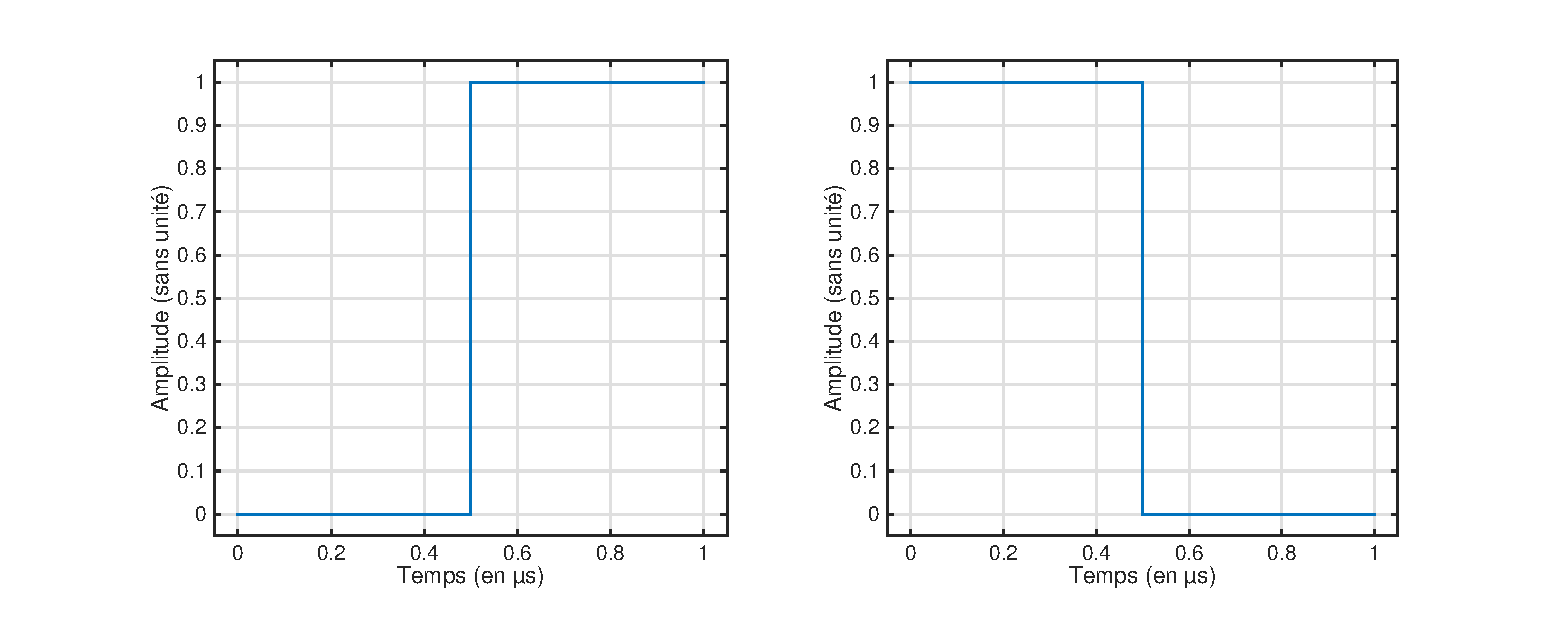
\includegraphics[scale=0.5]{impulsions.eps}
            \caption{$p_0(t)$ et $p_1(t)$}
    \end{figure}
    \noindent
    Le signal envoyé est le suivant : $ s_l(t) = \displaystyle\sum_{k \in \mathbb{Z}}{p_{b_k}\left(t-k\,T_s\right)} $ avec $p_{b_k} = \left\{ \begin{array}{ll}
            p_0(t) & \mbox{si $b_k = 0$}\\
            p_1(t) & \mbox{si $b_k = 1$}\end{array} \right.$
    
    \vspace{11pt}
    \noindent
    Nous prenons comme hypothèses :
    \renewcommand{\labelitemi}{\textbullet}
    \renewcommand{\labelitemii}{$\star$}
    \begin{itemize}
        \item Les $b_k$ sont indépendants et distribués uniformément,
        \item Le bruit $n_l(t) \sim \mathcal{N}_{\mathbb{R}}(0, \sigma^2_{n_l})$ a pour densité spectrale de puissance $\Gamma_{n_l}(f) = \frac{N_0}{2}$
        \item On considère l'architecture de communication ci-dessous :
    \end{itemize}

    \vspace{11pt}
    
    \begin{figure}[h!]
    \centering
    \psscalebox{0.6} % Change this value to rescale the drawing.
    {
        \begin{pspicture}(0,-2.9224317)(20.0,2.9224317)
            \psframe[linecolor=black, linewidth=0.04, dimen=outer](5.4,0.47756836)(2.0,-1.1224316)
            \psline[linecolor=black, linewidth=0.04, arrowsize=0.05291666666666667cm 2.0,arrowlength=1.4,arrowinset=0.0]{->}(0.8,-0.32243165)(2.0,-0.32243165)
            \psline[linecolor=black, linewidth=0.04, arrowsize=0.05291666666666667cm 2.0,arrowlength=1.4,arrowinset=0.0]{->}(5.4,-0.32243165)(7.2,-0.32243165)
            \pscircle[linecolor=black, linewidth=0.04, dimen=outer](7.6,-0.32243165){0.4}
            \psline[linecolor=black, linewidth=0.04](7.6,0.07756836)(7.6,-0.72243166)
            \psline[linecolor=black, linewidth=0.04](7.2,-0.32243165)(8.0,-0.32243165)
            \psline[linecolor=black, linewidth=0.04](8.0,-0.32243165)(9.0,-0.32243165)
            \psline[linecolor=black, linewidth=0.04, arrowsize=0.05291666666666667cm 2.0,arrowlength=1.4,arrowinset=0.0]{->}(9.0,-0.32243165)(9.0,1.8775684)(10.4,1.8775684)
            \psline[linecolor=black, linewidth=0.04, arrowsize=0.05291666666666667cm 2.0,arrowlength=1.4,arrowinset=0.0]{->}(9.0,-0.32243165)(9.0,-2.5224316)(10.4,-2.5224316)
            \psframe[linecolor=black, linewidth=0.04, dimen=outer](12.2,2.2775683)(10.4,1.4775684)
            \psframe[linecolor=black, linewidth=0.04, dimen=outer](12.2,-2.1224318)(10.4,-2.9224317)
            \psline[linecolor=black, linewidth=0.04](12.2,1.8775684)(13.32,1.8775684)(13.8,2.2775683)
            \psline[linecolor=black, linewidth=0.04](12.2,-2.5224316)(13.32,-2.5224316)(13.8,-2.1224318)
            \psline[linecolor=black, linewidth=0.04](13.8,1.8775684)(16.0,1.8775684)(16.0,1.6775683)
            \psline[linecolor=black, linewidth=0.04](13.8,-2.5224316)(16.0,-2.5224316)(16.0,-2.5224316)
            \psframe[linecolor=black, linewidth=0.04, dimen=outer](17.2,0.07756836)(15.4,-0.72243166)
            \psline[linecolor=black, linewidth=0.04, arrowsize=0.05291666666666667cm 2.0,arrowlength=1.4,arrowinset=0.0]{->}(16.0,1.6775683)(16.0,0.07756836)
            \psline[linecolor=black, linewidth=0.04, arrowsize=0.05291666666666667cm 2.0,arrowlength=1.4,arrowinset=0.0]{->}(16.0,-2.5224316)(16.0,-0.72243166)
            \psline[linecolor=black, linewidth=0.04, arrowsize=0.05291666666666667cm 2.0,arrowlength=1.4,arrowinset=0.0]{->}(17.2,-0.32243165)(18.2,-0.32243165)
            \rput[bl](2.8,-0.12243164){\large Modulation}
            \rput[bl](3.4,-0.72243166){\large PPM}
            \rput[bl](10.6,1.8775684){\large ${p_0}^*(-t)$}
            \rput[bl](10.6,-2.5224316){\large ${p_1}^*(-t)$}
            \rput[bl](13.8,2.6775684){$T_s$}
            \rput[bl](13.8,-1.9224316){$T_s$}
            \rput[bl](15.6,-0.32243165){\large argmax}
            \rput[bl](6.0,-0.12243164){$s_l(t)$}
            \rput[bl](8.0,-0.12243164){$y_l(t)$}
            \psline[linecolor=black, linewidth=0.04, arrowsize=0.05291666666666667cm 2.0,arrowlength=1.4,arrowinset=0.0]{->}(7.6,1.6775683)(7.6,0.07756836)
            \rput[bl](7.2,1.8775684){$n_l(t)$}
            \rput[bl](0.0,-0.32243165){$b_k$}
            \rput[bl](18.4,-0.32243165){$\hat{b}_k$}
            \rput[bl](16.4,0.87756836){$r_0(k)$}
            \rput[bl](16.4,-1.7224317){$r_1(k)$}
        \end{pspicture}
    }
    \caption{Chaîne de communication complète}
    \end{figure}
    
    \vspace{11pt}
    \noindent
    Par les graphes de $p(t)$, $p_0(t)$ et $p_1(t)$, on en déduit que 
    $s_l(t) = 0.5 + \displaystyle\sum_{k \in \mathbb{Z}}{A_k p\left(t-k\,T_s\right)}$ où $A_k = \left\{ \begin{array}{ll}
            \;1 & \mbox{si $b_k = 0$}\\
            -1 & \mbox{si $b_k = 1$}\end{array} \right.$
    
    \vspace{11pt}        
    \noindent
    Avec $s_l(t) - 0.5$, on obtient une modulation PAM.
    \noindent
    Après la modulation du signal et sa transmission à travers le canal, il est filtré après avoir été réceptionné par les filtres adaptés $p_0^*(-t)$ et $p_1^*(-t)$ tels que $p_0^*(-t) = p_0(t)$ et $p_1^*(-t) = p_1(t)$. De tels filtres permettent de diminuer l'influence du bruit introduit par le canal afin de maximiser le SNR, c'est-à-dire le rapport $\displaystyle\frac{v(0)}{\sigma}$, aux instants $n T_s$.
    
    \vspace{5pt}
    Pour que la transmission se fasse sans erreur donc pour que l'IES (interférence entre symboles) soit nulle, il faut que les couples de filtres ($p_0(t)$,$p_0^*(-t)$) et ($p_1(t)$,$p_1^*(-t)$) vérifient le critère de Nyquist.
    
    \vspace{5pt}
    \noindent
    Tout calcul fait, $\displaystyle v_0(t) = p_0(t) * p_0(-t) = 
    \left\{ \begin{array}{ll}
            \; t + \frac{T_s}{2} & \mbox{si }t \in \left[-\frac{T_s}{2},0\right]\\
            \frac{T_s}{2} - t & \mbox{si }t \in \left[0,\frac{T_s}{2}\right] \\
            0 &\mbox{ sinon} \end{array} \right.\;\; \Rightarrow \;\; v_0(t) \displaystyle\sum_{k \in \mathbb{Z}} \delta \left(t-k\,T_s\right) = \frac{1}{2} \delta(t)$.
    
    \vspace{5pt}
    \noindent
    Le couple $\left(p_0(t), p_0^*(-t)\right)$ vérifie donc bien le critère. De même, on vérifie que le couple $\left(p_1(t), p_1^*(-t)\right)$ respecte le critère de Nyquist.
    
\begin{figure}[h!]    
    \psscalebox{0.7} % Change this value to rescale the drawing.
    {
        \begin{pspicture}(-1,-1.364795)(18,1.364795)
            \psframe[linecolor=black, linewidth=0.04, dimen=outer](5.0,-0.08885742)(2.2,-1.2888575)
            \rput[bl](2.6,-0.68885744){Modulation}
            \rput[bl](3.2,-1.0888574){PPM}
            \psline[linecolor=black, linewidth=0.04, arrowsize=0.05291666666666667cm 2.0,arrowlength=1.4,arrowinset=0.0]{->}(5.0,-0.68885744)(6.2,-0.68885744)
            \pscircle[linecolor=black, linewidth=0.04, dimen=outer](6.6,-0.68885744){0.4}
            \psline[linecolor=black, linewidth=0.04](6.6,-0.28885743)(6.6,-1.0888574)
            \psline[linecolor=black, linewidth=0.04](6.2,-0.68885744)(7.0,-0.68885744)
            \psline[linecolor=black, linewidth=0.04, arrowsize=0.05291666666666667cm 2.0,arrowlength=1.4,arrowinset=0.0]{->}(1.0,-0.68885744)(2.2,-0.68885744)
            \psline[linecolor=black, linewidth=0.04, arrowsize=0.05291666666666667cm 2.0,arrowlength=1.4,arrowinset=0.0]{->}(6.6,0.7111426)(6.6,-0.28885743)
            \psline[linecolor=black, linewidth=0.04, arrowsize=0.05291666666666667cm 2.0,arrowlength=1.4,arrowinset=0.0]{->}(7.0,-0.68885744)(8.4,-0.68885744)
            \psframe[linecolor=black, linewidth=0.04, dimen=outer](10.2,-0.08885742)(8.4,-1.2888575)
            \psline[linecolor=black, linewidth=0.04](10.2,-0.68885744)(11.4,-0.68885744)(12.0,-0.28885743)
            \psline[linecolor=black, linewidth=0.04, arrowsize=0.05291666666666667cm 2.0,arrowlength=1.4,arrowinset=0.0]{->}(12.0,-0.68885744)(14.0,-0.68885744)
            \psframe[linecolor=black, linewidth=0.04, dimen=outer](15.8,-0.08885742)(14.0,-1.2888575)
            \psline[linecolor=black, linewidth=0.04, arrowsize=0.05291666666666667cm 2.0,arrowlength=1.4,arrowinset=0.0]{->}(15.8,-0.68885744)(17.0,-0.68885744)
            \rput[bl](9.0,-0.68885744){$p(t)$}
            \rput[bl](14.4,-0.68885744){signe}
            \rput[bl](0.0,-0.68885744){$b_k$}
            \rput[bl](5.4,-0.28885743){$s_l(t)$}
            \rput[bl](6.4,1.1111426){$n_l(t)$}
            \rput[bl](7.4,-0.28885743){$y_l(t)$}
            \rput[bl](11.4,-0.08885742){$T_s$}
            \rput[bl](12.4,-1.2888575){$r_0(k)$}
            \rput[bl](17.2,-0.68885744){$\hat{b_k}$}
        \end{pspicture}
    }
    \caption{Chaîne de communication équivalente
}
\end{figure}

    \vspace{11pt}
\noindent
    Pour calculer la densité spectrale de puissance (DSP) théorique de $s_l(t)$, nous passons par plusieurs étapes :
    
    \vspace{6pt}
    
    \begin{itemize}
        \item $ m_{s_l}(t) = \mathbb{E}\left[s_l(t)\right] = 0.5 + \displaystyle\sum_{k \in \mathbb{Z}} \mathbb{E}\left[A_k\right]\;p\left(t-k\,T_s\right) = 0.5$
        
        \vspace{6pt}
        car $\;\;\forall k \in \mathbb{Z}, \,\mathbb{E}\left[A_k\right] = 1 \cdot \underbrace{p\left(A_k = 0\right)}_{= \displaystyle0.5} + (-1) \cdot \underbrace{p\left(A_k = 1\right)}_{= \displaystyle0.5} = 0\;\;$ (les $b_k$ étant uniformément distribués)\\
        
        \vspace{7pt}
        \item \hspace{5pt}\\
            \vspace{-38.4pt}
            \begin{flalign*}
                R_{s_l}(t,\tau) &= \mathbb{E}\left[s_l(t) {s_l}^*(t+\tau)\right] &\\
                &= \mathbb{E}\left[\left(0.5+\sum_{k \in \mathbb{Z}} A_k p\left(t-k T_s\right)\right)\left(0.5+\sum_{l \in \mathbb{Z}} A_l p\left(t+\tau-l T_s\right)\right)\right] &\\
                &= 0.25 + 0.5 \sum_{k \in \mathbb{Z}} \underbrace{\mathbb{E} \left[A_k\right]}_{= 0} p(t+\tau-k T_s) + 0.5 \sum_{l \in \mathbb{Z}} \underbrace{\mathbb{E} \left[A_l\right]}_{= 0} p(t+\tau-l T_s) + \sum_{k, l \in \mathbb{Z}} \mathbb{E} \left[A_k A_l\right] p(t-l T_s)p(t+\tau-k T_s) &\\
                &= 0.25 + \sum_{k, l \in \mathbb{Z}} \underbrace{\mathbb{E} \left[A_k A_l\right]}_{= \delta_{k,l}} p(t-l T_s)p(t+\tau-k T_s) =  0.25 + \sum_{k \in \mathbb{Z}} p(t-k T_s)p(t+\tau-k T_s)&
        \end{flalign*}
        \vspace{3pt}
        \item Suite au calcul de $R_{s_l}(t, \tau)$, on montre que $s_l(t)$ est cyclo-stationnaire de cycle $T_s$:
            \begin{flalign*}
                \mathbb{E}\left[s_l(t+T_s) {s_l}^*(t+\tau+T_s)\right] &= 0.25 + \sum_{k \in \mathbb{Z}} \mathbb{E} \left[A_k\right] p(t+ T_s -k T_s)p(t+T_s+\tau - k T_s) &\\
                &= 0.25 + \sum_{k \in \mathbb{Z}} \mathbb{E} \left[A_k\right] p(t - (k-1) T_s)p(t + \tau - (k-1) T_s) &\\
                &= 0.25 + \sum_{k' \in \mathbb{Z}} \mathbb{E} \left[A_k\right] p(t - k' T_s)p(t + \tau - k' T_s) = \mathbb{E}\left[s_l(t) {s_l}^*(t+\tau)\right] &
            \end{flalign*}
        \item On peut maintenant en déduire l'autocorrélation moyennée $\tilde{R}_{s_l}(\tau)$ : 
        \begin{flalign*}
            \tilde{R}_{s_l}(\tau) &= \frac{1}{T_s} \int_0^{T_s} \left(0.25 + \sum_{k \in \mathbb{Z}} p(t-k T_s)p(t+\tau-k T_s) \right) dt &\\
            &= 0.25 + \frac{1}{T_s} \sum_{k \in \mathbb{Z}}\int_0^{T_s} \left( p(t-k T_s)p(t+\tau-k T_s) \right) dt &\\
            &=  0.25 + \frac{1}{T_s} \sum_{k \in \mathbb{Z}}\int_{-k T_s}^{(1-k) T_s} p(u)p(u+\tau) du \quad\mbox{ avec le changement de variable } u = t- k T_s &\\
            &= 0.25 + \frac{1}{T_s} \int_{-\infty}^{+\infty} p(u)p(u+\tau) du &\\
            &= 0.25 + \frac{1}{T_s} R_p(\tau) &
        \end{flalign*}
        \item Pour pouvoir tracer $\tilde{R}_{s_l}(\tau)$, nous devons calculer $\displaystyle R_p(\tau) = \int_{-\infty}^{+\infty} p(t)p\left(t+\tau\right)dt$
            \vspace{5pt}
            \begin{itemize}
                \item si $\displaystyle\tau \in \left[0,\frac{T_s}{2}\right], R_p(\tau) = \int_\tau^{\frac{T_s}{2}}\left(-0.5\right)^2 dt + \int_{\frac{T_s}{2}}^{\frac{T_s}{2}+\tau} 0.5 \cdot (-0.5) dt + \int_{\frac{T_s}{2}+\tau}^{T_s}\left(0.5\right)^2 dt = \frac{T_s}{4} - \frac{3 \tau}{4}$\\
                \item si $\tau \in \left[\displaystyle\frac{T_s}{2}, T_s\right], R_p(\tau) = -\int_\tau^{T_s} 0.25 dt = \displaystyle\frac{\tau - T_s}{4}$\\
            \end{itemize}
            \vspace{10pt}
            Ce qui donne la figure ci-dessous :
            \begin{figure}[h!]
            \centering
            % This file was created by matlab2tikz.
% Minimal pgfplots version: 1.3
%
%The latest updates can be retrieved from
%  http://www.mathworks.com/matlabcentral/fileexchange/22022-matlab2tikz
%where you can also make suggestions and rate matlab2tikz.
%
\definecolor{mycolor1}{rgb}{0.00000,0.44700,0.74100}%
%
\begin{tikzpicture}

\begin{axis}[%
width=3in,
height=2in,
at={(1.011111in,0.641667in)},
xmin=0,
xmax=2,
xlabel={$\frac{\tau}{T_s}$},
ymin=0,
ymax=0.5,
xmajorgrids,
ymajorgrids
]
\addplot [color=mycolor1,solid,forget plot]
  table[row sep=crcr]{%
0	0.5\\
0.1	0.425\\
0.2	0.35\\
0.3	0.275\\
0.4	0.2\\
0.5	0.125\\
0.6	0.15\\
0.7	0.175\\
0.8	0.2\\
0.9	0.225\\
1	0.25\\
1.1	0.25\\
1.2	0.25\\
1.3	0.25\\
1.4	0.25\\
1.5	0.25\\
1.6	0.25\\
1.7	0.25\\
1.8	0.25\\
1.9	0.25\\
2	0.25\\
};
\end{axis}
\end{tikzpicture}%
            \caption{Tracé de l'autocorrélation moyennée $\tilde{R}_{s_l}$}
            \end{figure}
        \item Enfin, calculons la DSP de $s_l(t)$ :
            \begin{flalign*}
                \Gamma_{s_l}(f) &= \mathcal{F}\left\{\tilde{R}_{s_l}(\tau)\right\} &\\
                &= 0.25 \, \delta(f) + \frac{\Gamma_p(f)}{T_s} &
            \end{flalign*}
            Calculons alors $\Gamma_p(f)$ :\\
            \vspace{3pt}
            $\displaystyle p'(t) = -0.5 \, \delta(t) + \delta\left(t-\frac{T_s}{2}\right)-0.5\,\delta\left(t-T_s\right) \\ \Rightarrow j2\pi f P(f) = -0.5 + \exp\left(-j\pi f T_s\right) - 0.5 \exp\left(-j 2\pi f T_s\right)$
            \begin{flalign*}
            \Rightarrow P(f) &= \frac{-0.5 \exp\left(-j 2 \pi f T_s\right) \left(\exp\left(j\pi f \frac{T_s}{2}\right) - \exp\left(-j\pi f \frac{T_s}{2}\right)\right)^2}{j 2 \pi f } &\\
            &= \frac{\pi f {T_s}^2}{4} \cdot \frac{\exp\left(\-j 2 \pi f T_s \right)}{j} \cdot\sinc\left(f \frac{T_s}{2}\right)^2 &
            \end{flalign*}
            $\displaystyle \Rightarrow \Gamma_p(f) = \frac{\pi^2 f^2 {T_s}^4}{16} \sinc\left(f \frac{T_s}{2}\right)^4$\\
            
            \vspace{3pt}
            \noindent
            D'où :
            \[ \boxed{\Gamma_{s_l}(f) = 0.25 \, \delta(f) + \frac{{\Pi}^2 f^2 {T_s}^3}{16} \sinc\left(f \frac{T_s}{2}\right)^4 } \]
    \end{itemize}
    
    \vspace{12pt}
    \noindent
    Après le filtrage adapté, on note $n'_{l,0}(t)$ et $n'_{l,1}(t)$ les bruits filtrés respectivement par ${p_0}^*(t)$ et ${p_1}^*(t)$.
    \begin{flalign*}
        R_{n'_{l,0}}(\tau) &= R_{n'_{l,0}}(-\tau) = n'_{l,0}(\tau) \ast n'_{l,0}(-\tau) &\\
        &= n_l(\tau) \ast p^*_0(-\tau) \ast n_l(-\tau) \ast p^*_0(\tau) = n_l(\tau) \ast n_l(-\tau) \ast p^*_0(-\tau) \ast p^*_0(\tau) &\\
        &= R_{n_l}(\tau) \ast R_{p_0}(\tau) = \frac{N_0}{2} R_{p_0}(\tau)&\\
    \end{flalign*}
    
    \newpage
    \begin{figure}[h!]
    \centering
    % This file was created by matlab2tikz.
% Minimal pgfplots version: 1.3
%
%The latest updates can be retrieved from
%  http://www.mathworks.com/matlabcentral/fileexchange/22022-matlab2tikz
%where you can also make suggestions and rate matlab2tikz.
%
\definecolor{mycolor1}{rgb}{0.00000,0.44700,0.74100}%
%
\begin{tikzpicture}

\begin{axis}[%
width=3in,
height=2in,
at={(1.011111in,0.641667in)},
xmin=-0.05,
xmax=2.05,
xlabel={$\frac{\tau}{T_s}$},
xmajorgrids,
ymin=-0.05,
ymax=1.05,
ylabel={\footnotesize Amplitude normalisée},
ymajorgrids
]
\addplot [color=mycolor1,solid,forget plot]
  table[row sep=crcr]{%
0	0\\
0.5	0\\
1	1\\
1.5	0\\
2	0\\
};
\end{axis}
\end{tikzpicture}%
    \caption{Tracé de $R_{n'_{l,0}}(\tau)$}
    \end{figure}
    
    Le processus aléatoire $n'_{l,0}(t)$ ne reste pas blanc (de même pour $n'_{l,1}(t)$). Néanmoins, l'échantillonnage de $R_{n'_{l,0}}$ au rythme $T_s$ donne un processus blanc. Les bruits filtrés et échantillonnés suivent alors une loi gaussienne échantillonnée $\displaystyle\mathcal{N}\left(0, E_p \frac{N_0}{2}\right)$ où $E_p = \displaystyle\frac{T_s}{2}$.
    
    \vspace{10pt}
    \noindent Déterminons alors le taux d'erreur binaire selon le rapport signal/bruit :
    \begin{flalign*}
        P_b &= \int_0^{+\infty} \frac{1}{\sqrt{\pi T_s \frac{N_0}{2}}}\exp\left(-\frac{2\left(x+\frac{T_s}{2}\right)^2}{T_s N_0}\right) dx = \int_{\sqrt{\frac{T_s}{2 N_0}}}^{+\infty} \frac{\exp\left(-v^2\right)}{\sqrt{\pi}} dv \qquad \text{avec }v = \sqrt{\frac{2}{T_s N_0}}\left(x+\frac{T_s}{2}\right) &\\
        &= \frac{1}{2} \erfc\left(\sqrt{\frac{T_s}{2 N_0}}\right) &
    \end{flalign*}
    Or $\displaystyle\quad E_b = P_{\text{moy}} T_b = \tilde{R}_{s_l}(0) T_s = \frac{T_s}{2}$\\
    D'où :
    \[
        \boxed{P_b = \frac{1}{2} \erfc\left(\sqrt{\frac{E_b}{N_0}}\right)}
    \]
    
    \subsection{Émission et réception de signaux modulés par une PPM}
    \noindent
    Nous vérifions dans cette partie les résultats obtenus dans la partie précédente.
    
    \begin{figure}[h!]
        \begin{minipage}[b]{.48\linewidth}
        	\centering
        	% This file was created by matlab2tikz.
% Minimal pgfplots version: 1.3
%
%The latest updates can be retrieved from
%  http://www.mathworks.com/matlabcentral/fileexchange/22022-matlab2tikz
%where you can also make suggestions and rate matlab2tikz.
%
\definecolor{mycolor1}{rgb}{0.00000,0.44700,0.74100}%
%
\begin{tikzpicture}

\begin{axis}[%
width=3in,
height=2.1in,
at={(1.011111in,0.641667in)},
xmin=-10,
xmax=510,
xlabel={\footnotesize temps (en $\mu s$)},
xmajorgrids,
ymin=-0.05,
ymax=1.05,
ymajorgrids
]
\addplot [color=mycolor1,solid,forget plot]
  table[row sep=crcr]{%
1	0\\
2	0\\
3	0\\
4	0\\
5	0\\
6	0\\
7	0\\
8	0\\
9	0\\
10	0\\
11	0\\
12	0\\
13	0\\
14	0\\
15	0\\
16	0\\
17	0\\
18	0\\
19	0\\
20	0\\
21	1\\
22	1\\
23	1\\
24	1\\
25	1\\
26	1\\
27	1\\
28	1\\
29	1\\
30	1\\
31	1\\
32	1\\
33	1\\
34	1\\
35	1\\
36	1\\
37	1\\
38	1\\
39	1\\
40	1\\
41	0\\
42	0\\
43	0\\
44	0\\
45	0\\
46	0\\
47	0\\
48	0\\
49	0\\
50	0\\
51	0\\
52	0\\
53	0\\
54	0\\
55	0\\
56	0\\
57	0\\
58	0\\
59	0\\
60	0\\
61	1\\
62	1\\
63	1\\
64	1\\
65	1\\
66	1\\
67	1\\
68	1\\
69	1\\
70	1\\
71	0\\
72	0\\
73	0\\
74	0\\
75	0\\
76	0\\
77	0\\
78	0\\
79	0\\
80	0\\
81	1\\
82	1\\
83	1\\
84	1\\
85	1\\
86	1\\
87	1\\
88	1\\
89	1\\
90	1\\
91	0\\
92	0\\
93	0\\
94	0\\
95	0\\
96	0\\
97	0\\
98	0\\
99	0\\
100	0\\
101	1\\
102	1\\
103	1\\
104	1\\
105	1\\
106	1\\
107	1\\
108	1\\
109	1\\
110	1\\
111	1\\
112	1\\
113	1\\
114	1\\
115	1\\
116	1\\
117	1\\
118	1\\
119	1\\
120	1\\
121	0\\
122	0\\
123	0\\
124	0\\
125	0\\
126	0\\
127	0\\
128	0\\
129	0\\
130	0\\
131	1\\
132	1\\
133	1\\
134	1\\
135	1\\
136	1\\
137	1\\
138	1\\
139	1\\
140	1\\
141	0\\
142	0\\
143	0\\
144	0\\
145	0\\
146	0\\
147	0\\
148	0\\
149	0\\
150	0\\
151	1\\
152	1\\
153	1\\
154	1\\
155	1\\
156	1\\
157	1\\
158	1\\
159	1\\
160	1\\
161	0\\
162	0\\
163	0\\
164	0\\
165	0\\
166	0\\
167	0\\
168	0\\
169	0\\
170	0\\
171	0\\
172	0\\
173	0\\
174	0\\
175	0\\
176	0\\
177	0\\
178	0\\
179	0\\
180	0\\
181	1\\
182	1\\
183	1\\
184	1\\
185	1\\
186	1\\
187	1\\
188	1\\
189	1\\
190	1\\
191	1\\
192	1\\
193	1\\
194	1\\
195	1\\
196	1\\
197	1\\
198	1\\
199	1\\
200	1\\
201	0\\
202	0\\
203	0\\
204	0\\
205	0\\
206	0\\
207	0\\
208	0\\
209	0\\
210	0\\
211	0\\
212	0\\
213	0\\
214	0\\
215	0\\
216	0\\
217	0\\
218	0\\
219	0\\
220	0\\
221	1\\
222	1\\
223	1\\
224	1\\
225	1\\
226	1\\
227	1\\
228	1\\
229	1\\
230	1\\
231	0\\
232	0\\
233	0\\
234	0\\
235	0\\
236	0\\
237	0\\
238	0\\
239	0\\
240	0\\
241	1\\
242	1\\
243	1\\
244	1\\
245	1\\
246	1\\
247	1\\
248	1\\
249	1\\
250	1\\
251	0\\
252	0\\
253	0\\
254	0\\
255	0\\
256	0\\
257	0\\
258	0\\
259	0\\
260	0\\
261	1\\
262	1\\
263	1\\
264	1\\
265	1\\
266	1\\
267	1\\
268	1\\
269	1\\
270	1\\
271	1\\
272	1\\
273	1\\
274	1\\
275	1\\
276	1\\
277	1\\
278	1\\
279	1\\
280	1\\
281	0\\
282	0\\
283	0\\
284	0\\
285	0\\
286	0\\
287	0\\
288	0\\
289	0\\
290	0\\
291	1\\
292	1\\
293	1\\
294	1\\
295	1\\
296	1\\
297	1\\
298	1\\
299	1\\
300	1\\
301	0\\
302	0\\
303	0\\
304	0\\
305	0\\
306	0\\
307	0\\
308	0\\
309	0\\
310	0\\
311	1\\
312	1\\
313	1\\
314	1\\
315	1\\
316	1\\
317	1\\
318	1\\
319	1\\
320	1\\
321	0\\
322	0\\
323	0\\
324	0\\
325	0\\
326	0\\
327	0\\
328	0\\
329	0\\
330	0\\
331	0\\
332	0\\
333	0\\
334	0\\
335	0\\
336	0\\
337	0\\
338	0\\
339	0\\
340	0\\
341	1\\
342	1\\
343	1\\
344	1\\
345	1\\
346	1\\
347	1\\
348	1\\
349	1\\
350	1\\
351	1\\
352	1\\
353	1\\
354	1\\
355	1\\
356	1\\
357	1\\
358	1\\
359	1\\
360	1\\
361	0\\
362	0\\
363	0\\
364	0\\
365	0\\
366	0\\
367	0\\
368	0\\
369	0\\
370	0\\
371	0\\
372	0\\
373	0\\
374	0\\
375	0\\
376	0\\
377	0\\
378	0\\
379	0\\
380	0\\
381	1\\
382	1\\
383	1\\
384	1\\
385	1\\
386	1\\
387	1\\
388	1\\
389	1\\
390	1\\
391	1\\
392	1\\
393	1\\
394	1\\
395	1\\
396	1\\
397	1\\
398	1\\
399	1\\
400	1\\
401	0\\
402	0\\
403	0\\
404	0\\
405	0\\
406	0\\
407	0\\
408	0\\
409	0\\
410	0\\
411	1\\
412	1\\
413	1\\
414	1\\
415	1\\
416	1\\
417	1\\
418	1\\
419	1\\
420	1\\
421	0\\
422	0\\
423	0\\
424	0\\
425	0\\
426	0\\
427	0\\
428	0\\
429	0\\
430	0\\
431	1\\
432	1\\
433	1\\
434	1\\
435	1\\
436	1\\
437	1\\
438	1\\
439	1\\
440	1\\
441	0\\
442	0\\
443	0\\
444	0\\
445	0\\
446	0\\
447	0\\
448	0\\
449	0\\
450	0\\
451	1\\
452	1\\
453	1\\
454	1\\
455	1\\
456	1\\
457	1\\
458	1\\
459	1\\
460	1\\
461	0\\
462	0\\
463	0\\
464	0\\
465	0\\
466	0\\
467	0\\
468	0\\
469	0\\
470	0\\
471	0\\
472	0\\
473	0\\
474	0\\
475	0\\
476	0\\
477	0\\
478	0\\
479	0\\
480	0\\
481	1\\
482	1\\
483	1\\
484	1\\
485	1\\
486	1\\
487	1\\
488	1\\
489	1\\
490	1\\
491	0\\
492	0\\
493	0\\
494	0\\
495	0\\
496	0\\
497	0\\
498	0\\
499	0\\
500	0\\
};
\end{axis}
\end{tikzpicture}%
            \caption{$s_l(t)$ pour les 25 premiers bits envoyés aléatoirement}
        \end{minipage} \hfill
        \begin{minipage}[b]{.48\linewidth}
        	\centering
        	% This file was created by matlab2tikz.
% Minimal pgfplots version: 1.3
%
%The latest updates can be retrieved from
%  http://www.mathworks.com/matlabcentral/fileexchange/22022-matlab2tikz
%where you can also make suggestions and rate matlab2tikz.
%
\definecolor{mycolor1}{rgb}{0.00000,0.44706,0.74118}%
%
\begin{tikzpicture}

\begin{axis}[%
width=3in,
height=2.1in,
at={(1.4625in,0.670694in)},
unbounded coords=jump,
xmin=-1,
xmax=1,
xlabel={\footnotesize temps (en $\mu s$)},
ymin=-0.05,
ymax=1.05
]
\addplot [color=mycolor1,solid,forget plot]
  table[row sep=crcr]{%
0	1\\
5e-02	1\\
1e-01	1\\
1.5e-01	1\\
2e-01	1\\
2.5e-01	1\\
3e-01	1\\
3.5e-01	1\\
4e-01	1\\
4.5e-01	1\\
5e-01	0\\
5.5e-01	0\\
6e-01	0\\
6.5e-01	0\\
7e-01	0\\
7.5e-01	0\\
8e-01	0\\
8.5e-01	0\\
9e-01	0\\
9.5e-01	0\\
1	1\\
nan	nan\\
-1	1\\
-9.5e-01	1\\
-9e-01	1\\
-8.5e-01	1\\
-8e-01	1\\
-7.5e-01	1\\
-7e-01	1\\
-6.5e-01	1\\
-6e-01	1\\
-5.5e-01	1\\
-5e-01	1\\
-4.5e-01	1\\
-4e-01	1\\
-3.5e-01	1\\
-3e-01	1\\
-2.5e-01	1\\
-2e-01	1\\
-1.5e-01	1\\
-1e-01	1\\
-5e-02	1\\
0	0\\
4.99999999999998e-02	0\\
1e-01	0\\
1.5e-01	0\\
2e-01	0\\
2.5e-01	0\\
3e-01	0\\
3.5e-01	0\\
4e-01	0\\
4.5e-01	0\\
5e-01	1\\
5.5e-01	1\\
6e-01	1\\
6.5e-01	1\\
7e-01	1\\
7.5e-01	1\\
8e-01	1\\
8.5e-01	1\\
9e-01	1\\
9.5e-01	1\\
1	0\\
nan	nan\\
-1	0\\
-9.5e-01	0\\
-9e-01	0\\
-8.5e-01	0\\
-8e-01	0\\
-7.5e-01	0\\
-7e-01	0\\
-6.5e-01	0\\
-6e-01	0\\
-5.5e-01	0\\
-5e-01	1\\
-4.5e-01	1\\
-4e-01	1\\
-3.5e-01	1\\
-3e-01	1\\
-2.5e-01	1\\
-2e-01	1\\
-1.5e-01	1\\
-1e-01	1\\
-4.99999999999998e-02	1\\
0	0\\
4.99999999999998e-02	0\\
9.99999999999996e-02	0\\
1.5e-01	0\\
2e-01	0\\
2.5e-01	0\\
3e-01	0\\
3.5e-01	0\\
4e-01	0\\
4.5e-01	0\\
5e-01	1\\
5.5e-01	1\\
6e-01	1\\
6.5e-01	1\\
7e-01	1\\
7.5e-01	1\\
8e-01	1\\
8.5e-01	1\\
9e-01	1\\
9.5e-01	1\\
1	0\\
nan	nan\\
-1	0\\
-9.5e-01	0\\
-9e-01	0\\
-8.5e-01	0\\
-8e-01	0\\
-7.5e-01	0\\
-7e-01	0\\
-6.5e-01	0\\
-6e-01	0\\
-5.5e-01	0\\
-5e-01	0\\
-4.5e-01	0\\
-4e-01	0\\
-3.5e-01	0\\
-3e-01	0\\
-2.5e-01	0\\
-2e-01	0\\
-1.5e-01	0\\
-9.99999999999996e-02	0\\
-4.99999999999998e-02	0\\
0	1\\
4.99999999999998e-02	1\\
9.99999999999996e-02	1\\
1.5e-01	1\\
2e-01	1\\
2.5e-01	1\\
3e-01	1\\
3.5e-01	1\\
4e-01	1\\
4.5e-01	1\\
5e-01	1\\
5.5e-01	1\\
6e-01	1\\
6.5e-01	1\\
7e-01	1\\
7.5e-01	1\\
8e-01	1\\
8.5e-01	1\\
9e-01	1\\
9.5e-01	1\\
1	0\\
nan	nan\\
-1	0\\
-9.5e-01	0\\
-9e-01	0\\
-8.5e-01	0\\
-8e-01	0\\
-7.5e-01	0\\
-7e-01	0\\
-6.5e-01	0\\
-6e-01	0\\
-5.5e-01	0\\
-5e-01	0\\
-4.5e-01	0\\
-4e-01	0\\
-3.5e-01	0\\
-3e-01	0\\
-2.5e-01	0\\
-2e-01	0\\
-1.5e-01	0\\
-9.99999999999996e-02	0\\
-4.99999999999998e-02	0\\
0	1\\
5.00000000000007e-02	1\\
9.99999999999996e-02	1\\
1.5e-01	1\\
1.99999999999999e-01	1\\
2.5e-01	1\\
3.00000000000001e-01	1\\
3.5e-01	1\\
4e-01	1\\
4.49999999999999e-01	1\\
5e-01	0\\
5.50000000000001e-01	0\\
6e-01	0\\
6.5e-01	0\\
6.99999999999999e-01	0\\
7.5e-01	0\\
8.00000000000001e-01	0\\
8.5e-01	0\\
9e-01	0\\
9.49999999999999e-01	0\\
1	1\\
nan	nan\\
-9.99999999999999e-01	1\\
-9.49999999999999e-01	1\\
-9e-01	1\\
-8.5e-01	1\\
-8.00000000000001e-01	1\\
-7.5e-01	1\\
-6.99999999999999e-01	1\\
-6.5e-01	1\\
-6e-01	1\\
-5.50000000000001e-01	1\\
-5e-01	1\\
-4.49999999999999e-01	1\\
-4e-01	1\\
-3.5e-01	1\\
-3.00000000000001e-01	1\\
-2.5e-01	1\\
-1.99999999999999e-01	1\\
-1.5e-01	1\\
-9.99999999999996e-02	1\\
-5.00000000000007e-02	1\\
0	0\\
5.00000000000007e-02	0\\
9.99999999999996e-02	0\\
1.5e-01	0\\
1.99999999999999e-01	0\\
2.5e-01	0\\
3.00000000000001e-01	0\\
3.5e-01	0\\
4e-01	0\\
4.49999999999999e-01	0\\
5e-01	1\\
5.50000000000001e-01	1\\
6e-01	1\\
6.5e-01	1\\
6.99999999999999e-01	1\\
7.5e-01	1\\
8.00000000000001e-01	1\\
8.5e-01	1\\
9e-01	1\\
9.49999999999999e-01	1\\
1	0\\
nan	nan\\
-9.99999999999999e-01	0\\
-9.49999999999999e-01	0\\
-9e-01	0\\
-8.5e-01	0\\
-8.00000000000001e-01	0\\
-7.5e-01	0\\
-6.99999999999999e-01	0\\
-6.5e-01	0\\
-6e-01	0\\
-5.50000000000001e-01	0\\
-5e-01	1\\
-4.49999999999999e-01	1\\
-4e-01	1\\
-3.5e-01	1\\
-3.00000000000001e-01	1\\
-2.5e-01	1\\
-1.99999999999999e-01	1\\
-1.5e-01	1\\
-9.99999999999996e-02	1\\
-5.00000000000007e-02	1\\
0	0\\
5.00000000000007e-02	0\\
9.99999999999996e-02	0\\
1.5e-01	0\\
1.99999999999999e-01	0\\
2.5e-01	0\\
3.00000000000001e-01	0\\
3.5e-01	0\\
4e-01	0\\
4.49999999999999e-01	0\\
5e-01	1\\
5.50000000000001e-01	1\\
6e-01	1\\
6.5e-01	1\\
6.99999999999999e-01	1\\
7.5e-01	1\\
8.00000000000001e-01	1\\
8.5e-01	1\\
9e-01	1\\
9.49999999999999e-01	1\\
1	0\\
nan	nan\\
-9.99999999999999e-01	0\\
-9.49999999999999e-01	0\\
-9e-01	0\\
-8.5e-01	0\\
-8.00000000000001e-01	0\\
-7.5e-01	0\\
-6.99999999999999e-01	0\\
-6.5e-01	0\\
-6e-01	0\\
-5.50000000000001e-01	0\\
-5e-01	1\\
-4.49999999999999e-01	1\\
-4e-01	1\\
-3.5e-01	1\\
-3.00000000000001e-01	1\\
-2.5e-01	1\\
-1.99999999999999e-01	1\\
-1.5e-01	1\\
-9.99999999999996e-02	1\\
-5.00000000000007e-02	1\\
0	0\\
5.00000000000007e-02	0\\
9.99999999999996e-02	0\\
1.5e-01	0\\
1.99999999999999e-01	0\\
2.5e-01	0\\
3.00000000000001e-01	0\\
3.5e-01	0\\
4e-01	0\\
4.49999999999999e-01	0\\
5e-01	0\\
5.50000000000001e-01	0\\
6e-01	0\\
6.5e-01	0\\
6.99999999999999e-01	0\\
7.5e-01	0\\
8.00000000000001e-01	0\\
8.5e-01	0\\
9e-01	0\\
9.49999999999999e-01	0\\
1	1\\
nan	nan\\
-9.99999999999999e-01	1\\
-9.49999999999999e-01	1\\
-9e-01	1\\
-8.5e-01	1\\
-8.00000000000001e-01	1\\
-7.5e-01	1\\
-6.99999999999999e-01	1\\
-6.5e-01	1\\
-6e-01	1\\
-5.50000000000001e-01	1\\
-5e-01	1\\
-4.49999999999999e-01	1\\
-4e-01	1\\
-3.5e-01	1\\
-3.00000000000001e-01	1\\
-2.5e-01	1\\
-1.99999999999999e-01	1\\
-1.5e-01	1\\
-9.99999999999996e-02	1\\
-5.00000000000007e-02	1\\
0	0\\
5.00000000000007e-02	0\\
1.00000000000001e-01	0\\
1.49999999999999e-01	0\\
1.99999999999999e-01	0\\
2.5e-01	0\\
3.00000000000001e-01	0\\
3.50000000000001e-01	0\\
3.99999999999999e-01	0\\
4.49999999999999e-01	0\\
5e-01	1\\
5.50000000000001e-01	1\\
6.00000000000001e-01	1\\
6.49999999999999e-01	1\\
6.99999999999999e-01	1\\
7.5e-01	1\\
8.00000000000001e-01	1\\
8.50000000000001e-01	1\\
8.99999999999999e-01	1\\
9.49999999999999e-01	1\\
1	0\\
nan	nan\\
-9.99999999999999e-01	0\\
-9.49999999999999e-01	0\\
-8.99999999999999e-01	0\\
-8.50000000000001e-01	0\\
-8.00000000000001e-01	0\\
-7.5e-01	0\\
-6.99999999999999e-01	0\\
-6.49999999999999e-01	0\\
-6.00000000000001e-01	0\\
-5.50000000000001e-01	0\\
-5e-01	0\\
-4.49999999999999e-01	0\\
-3.99999999999999e-01	0\\
-3.50000000000001e-01	0\\
-3.00000000000001e-01	0\\
-2.5e-01	0\\
-1.99999999999999e-01	0\\
-1.49999999999999e-01	0\\
-1.00000000000001e-01	0\\
-5.00000000000007e-02	0\\
0	1\\
5.00000000000007e-02	1\\
1.00000000000001e-01	1\\
1.49999999999999e-01	1\\
1.99999999999999e-01	1\\
2.5e-01	1\\
3.00000000000001e-01	1\\
3.50000000000001e-01	1\\
3.99999999999999e-01	1\\
4.49999999999999e-01	1\\
5e-01	1\\
5.50000000000001e-01	1\\
6.00000000000001e-01	1\\
6.49999999999999e-01	1\\
6.99999999999999e-01	1\\
7.5e-01	1\\
8.00000000000001e-01	1\\
8.50000000000001e-01	1\\
8.99999999999999e-01	1\\
9.49999999999999e-01	1\\
1	0\\
nan	nan\\
-9.99999999999999e-01	0\\
-9.49999999999999e-01	0\\
-8.99999999999999e-01	0\\
-8.50000000000001e-01	0\\
-8.00000000000001e-01	0\\
-7.5e-01	0\\
-6.99999999999999e-01	0\\
-6.49999999999999e-01	0\\
-6.00000000000001e-01	0\\
-5.50000000000001e-01	0\\
-5e-01	0\\
-4.49999999999999e-01	0\\
-3.99999999999999e-01	0\\
-3.50000000000001e-01	0\\
-3.00000000000001e-01	0\\
-2.5e-01	0\\
-1.99999999999999e-01	0\\
-1.49999999999999e-01	0\\
-1.00000000000001e-01	0\\
-5.00000000000007e-02	0\\
0	1\\
5.00000000000007e-02	1\\
1.00000000000001e-01	1\\
1.49999999999999e-01	1\\
1.99999999999999e-01	1\\
2.5e-01	1\\
3.00000000000001e-01	1\\
3.50000000000001e-01	1\\
3.99999999999999e-01	1\\
4.49999999999999e-01	1\\
5e-01	0\\
5.50000000000001e-01	0\\
6.00000000000001e-01	0\\
6.49999999999999e-01	0\\
6.99999999999999e-01	0\\
7.5e-01	0\\
8.00000000000001e-01	0\\
8.50000000000001e-01	0\\
8.99999999999999e-01	0\\
9.49999999999999e-01	0\\
1	1\\
nan	nan\\
-9.99999999999999e-01	1\\
-9.49999999999999e-01	1\\
-8.99999999999999e-01	1\\
-8.50000000000001e-01	1\\
-8.00000000000001e-01	1\\
-7.5e-01	1\\
-6.99999999999999e-01	1\\
-6.49999999999999e-01	1\\
-6.00000000000001e-01	1\\
-5.50000000000001e-01	1\\
-5e-01	1\\
-4.49999999999999e-01	1\\
-3.99999999999999e-01	1\\
-3.50000000000001e-01	1\\
-3.00000000000001e-01	1\\
-2.5e-01	1\\
-1.99999999999999e-01	1\\
-1.49999999999999e-01	1\\
-1.00000000000001e-01	1\\
-5.00000000000007e-02	1\\
0	0\\
5.00000000000007e-02	0\\
1.00000000000001e-01	0\\
1.49999999999999e-01	0\\
1.99999999999999e-01	0\\
2.5e-01	0\\
3.00000000000001e-01	0\\
3.50000000000001e-01	0\\
3.99999999999999e-01	0\\
4.49999999999999e-01	0\\
5e-01	0\\
5.50000000000001e-01	0\\
6.00000000000001e-01	0\\
6.49999999999999e-01	0\\
6.99999999999999e-01	0\\
7.5e-01	0\\
8.00000000000001e-01	0\\
8.50000000000001e-01	0\\
8.99999999999999e-01	0\\
9.49999999999999e-01	0\\
1	1\\
nan	nan\\
-9.99999999999999e-01	1\\
-9.49999999999999e-01	1\\
-8.99999999999999e-01	1\\
-8.50000000000001e-01	1\\
-8.00000000000001e-01	1\\
-7.5e-01	1\\
-6.99999999999999e-01	1\\
-6.49999999999999e-01	1\\
-6.00000000000001e-01	1\\
-5.50000000000001e-01	1\\
-5e-01	1\\
-4.49999999999999e-01	1\\
-3.99999999999999e-01	1\\
-3.50000000000001e-01	1\\
-3.00000000000001e-01	1\\
-2.5e-01	1\\
-1.99999999999999e-01	1\\
-1.49999999999999e-01	1\\
-1.00000000000001e-01	1\\
-5.00000000000007e-02	1\\
0	0\\
5.00000000000007e-02	0\\
1.00000000000001e-01	0\\
1.49999999999999e-01	0\\
1.99999999999999e-01	0\\
2.5e-01	0\\
3.00000000000001e-01	0\\
3.50000000000001e-01	0\\
3.99999999999999e-01	0\\
4.49999999999999e-01	0\\
5e-01	1\\
5.50000000000001e-01	1\\
6.00000000000001e-01	1\\
6.49999999999999e-01	1\\
6.99999999999999e-01	1\\
7.5e-01	1\\
8.00000000000001e-01	1\\
8.50000000000001e-01	1\\
8.99999999999999e-01	1\\
9.49999999999999e-01	1\\
1	0\\
nan	nan\\
-9.99999999999999e-01	0\\
-9.49999999999999e-01	0\\
-8.99999999999999e-01	0\\
-8.50000000000001e-01	0\\
-8.00000000000001e-01	0\\
-7.5e-01	0\\
-6.99999999999999e-01	0\\
-6.49999999999999e-01	0\\
-6.00000000000001e-01	0\\
-5.50000000000001e-01	0\\
-5e-01	0\\
-4.49999999999999e-01	0\\
-3.99999999999999e-01	0\\
-3.50000000000001e-01	0\\
-3.00000000000001e-01	0\\
-2.5e-01	0\\
-1.99999999999999e-01	0\\
-1.49999999999999e-01	0\\
-1.00000000000001e-01	0\\
-5.00000000000007e-02	0\\
0	1\\
5.00000000000007e-02	1\\
1.00000000000001e-01	1\\
1.49999999999999e-01	1\\
1.99999999999999e-01	1\\
2.5e-01	1\\
3.00000000000001e-01	1\\
3.50000000000001e-01	1\\
3.99999999999999e-01	1\\
4.49999999999999e-01	1\\
5e-01	0\\
5.50000000000001e-01	0\\
6.00000000000001e-01	0\\
6.49999999999999e-01	0\\
6.99999999999999e-01	0\\
7.5e-01	0\\
8.00000000000001e-01	0\\
8.50000000000001e-01	0\\
8.99999999999999e-01	0\\
9.49999999999999e-01	0\\
1	1\\
nan	nan\\
-9.99999999999999e-01	1\\
-9.49999999999999e-01	1\\
-8.99999999999999e-01	1\\
-8.50000000000001e-01	1\\
-8.00000000000001e-01	1\\
-7.5e-01	1\\
-6.99999999999999e-01	1\\
-6.49999999999999e-01	1\\
-6.00000000000001e-01	1\\
-5.50000000000001e-01	1\\
-5e-01	0\\
-4.49999999999999e-01	0\\
-3.99999999999999e-01	0\\
-3.50000000000001e-01	0\\
-3.00000000000001e-01	0\\
-2.5e-01	0\\
-1.99999999999999e-01	0\\
-1.49999999999999e-01	0\\
-1.00000000000001e-01	0\\
-5.00000000000007e-02	0\\
0	1\\
5.00000000000007e-02	1\\
1.00000000000001e-01	1\\
1.49999999999999e-01	1\\
1.99999999999999e-01	1\\
2.5e-01	1\\
3.00000000000001e-01	1\\
3.50000000000001e-01	1\\
3.99999999999999e-01	1\\
4.49999999999999e-01	1\\
5e-01	1\\
5.50000000000001e-01	1\\
6.00000000000001e-01	1\\
6.49999999999999e-01	1\\
6.99999999999999e-01	1\\
7.5e-01	1\\
8.00000000000001e-01	1\\
8.50000000000001e-01	1\\
8.99999999999999e-01	1\\
9.49999999999999e-01	1\\
1	0\\
nan	nan\\
-9.99999999999999e-01	0\\
-9.49999999999999e-01	0\\
-8.99999999999999e-01	0\\
-8.50000000000001e-01	0\\
-8.00000000000001e-01	0\\
-7.5e-01	0\\
-6.99999999999999e-01	0\\
-6.49999999999999e-01	0\\
-6.00000000000001e-01	0\\
-5.50000000000001e-01	0\\
-5e-01	1\\
-4.49999999999999e-01	1\\
-3.99999999999999e-01	1\\
-3.50000000000001e-01	1\\
-3.00000000000001e-01	1\\
-2.5e-01	1\\
-1.99999999999999e-01	1\\
-1.49999999999999e-01	1\\
-1.00000000000001e-01	1\\
-5.00000000000007e-02	1\\
0	0\\
5.00000000000007e-02	0\\
1.00000000000001e-01	0\\
1.49999999999999e-01	0\\
1.99999999999999e-01	0\\
2.5e-01	0\\
3.00000000000001e-01	0\\
3.50000000000001e-01	0\\
3.99999999999999e-01	0\\
4.49999999999999e-01	0\\
5e-01	0\\
5.50000000000001e-01	0\\
6.00000000000001e-01	0\\
6.49999999999999e-01	0\\
6.99999999999999e-01	0\\
7.5e-01	0\\
8.00000000000001e-01	0\\
8.50000000000001e-01	0\\
8.99999999999999e-01	0\\
9.49999999999999e-01	0\\
1	1\\
nan	nan\\
-9.99999999999999e-01	1\\
-9.49999999999999e-01	1\\
-8.99999999999999e-01	1\\
-8.50000000000001e-01	1\\
-8.00000000000001e-01	1\\
-7.5e-01	1\\
-6.99999999999999e-01	1\\
-6.49999999999999e-01	1\\
-6.00000000000001e-01	1\\
-5.50000000000001e-01	1\\
-5e-01	0\\
-4.49999999999999e-01	0\\
-3.99999999999999e-01	0\\
-3.50000000000001e-01	0\\
-3.00000000000001e-01	0\\
-2.5e-01	0\\
-1.99999999999999e-01	0\\
-1.49999999999999e-01	0\\
-1.00000000000001e-01	0\\
-5.00000000000007e-02	0\\
0	1\\
4.99999999999972e-02	1\\
1.00000000000001e-01	1\\
1.49999999999999e-01	1\\
2.00000000000003e-01	1\\
2.5e-01	1\\
2.99999999999997e-01	1\\
3.50000000000001e-01	1\\
3.99999999999999e-01	1\\
4.50000000000003e-01	1\\
5e-01	1\\
5.49999999999997e-01	1\\
6.00000000000001e-01	1\\
6.49999999999999e-01	1\\
7.00000000000003e-01	1\\
7.5e-01	1\\
7.99999999999997e-01	1\\
8.50000000000001e-01	1\\
8.99999999999999e-01	1\\
9.50000000000003e-01	1\\
1	0\\
nan	nan\\
-1	0\\
-9.50000000000003e-01	0\\
-8.99999999999999e-01	0\\
-8.50000000000001e-01	0\\
-7.99999999999997e-01	0\\
-7.5e-01	0\\
-7.00000000000003e-01	0\\
-6.49999999999999e-01	0\\
-6.00000000000001e-01	0\\
-5.49999999999997e-01	0\\
-5e-01	1\\
-4.50000000000003e-01	1\\
-3.99999999999999e-01	1\\
-3.50000000000001e-01	1\\
-2.99999999999997e-01	1\\
-2.5e-01	1\\
-2.00000000000003e-01	1\\
-1.49999999999999e-01	1\\
-1.00000000000001e-01	1\\
-4.99999999999972e-02	1\\
0	0\\
4.99999999999972e-02	0\\
1.00000000000001e-01	0\\
1.49999999999999e-01	0\\
2.00000000000003e-01	0\\
2.5e-01	0\\
2.99999999999997e-01	0\\
3.50000000000001e-01	0\\
3.99999999999999e-01	0\\
4.50000000000003e-01	0\\
5e-01	0\\
5.49999999999997e-01	0\\
6.00000000000001e-01	0\\
6.49999999999999e-01	0\\
7.00000000000003e-01	0\\
7.5e-01	0\\
7.99999999999997e-01	0\\
8.50000000000001e-01	0\\
8.99999999999999e-01	0\\
9.50000000000003e-01	0\\
1	1\\
nan	nan\\
-1	1\\
-9.50000000000003e-01	1\\
-8.99999999999999e-01	1\\
-8.50000000000001e-01	1\\
-7.99999999999997e-01	1\\
-7.5e-01	1\\
-7.00000000000003e-01	1\\
-6.49999999999999e-01	1\\
-6.00000000000001e-01	1\\
-5.49999999999997e-01	1\\
-5e-01	1\\
-4.50000000000003e-01	1\\
-3.99999999999999e-01	1\\
-3.50000000000001e-01	1\\
-2.99999999999997e-01	1\\
-2.5e-01	1\\
-2.00000000000003e-01	1\\
-1.49999999999999e-01	1\\
-1.00000000000001e-01	1\\
-4.99999999999972e-02	1\\
0	0\\
4.99999999999972e-02	0\\
1.00000000000001e-01	0\\
1.49999999999999e-01	0\\
2.00000000000003e-01	0\\
2.5e-01	0\\
2.99999999999997e-01	0\\
3.50000000000001e-01	0\\
3.99999999999999e-01	0\\
4.50000000000003e-01	0\\
5e-01	0\\
5.49999999999997e-01	0\\
6.00000000000001e-01	0\\
6.49999999999999e-01	0\\
7.00000000000003e-01	0\\
7.5e-01	0\\
7.99999999999997e-01	0\\
8.50000000000001e-01	0\\
8.99999999999999e-01	0\\
9.50000000000003e-01	0\\
1	1\\
nan	nan\\
-1	1\\
-9.50000000000003e-01	1\\
-8.99999999999999e-01	1\\
-8.50000000000001e-01	1\\
-7.99999999999997e-01	1\\
-7.5e-01	1\\
-7.00000000000003e-01	1\\
-6.49999999999999e-01	1\\
-6.00000000000001e-01	1\\
-5.49999999999997e-01	1\\
-5e-01	0\\
-4.50000000000003e-01	0\\
-3.99999999999999e-01	0\\
-3.50000000000001e-01	0\\
-2.99999999999997e-01	0\\
-2.5e-01	0\\
-2.00000000000003e-01	0\\
-1.49999999999999e-01	0\\
-1.00000000000001e-01	0\\
-4.99999999999972e-02	0\\
0	1\\
4.99999999999972e-02	1\\
1.00000000000001e-01	1\\
1.49999999999999e-01	1\\
2.00000000000003e-01	1\\
2.5e-01	1\\
2.99999999999997e-01	1\\
3.50000000000001e-01	1\\
3.99999999999999e-01	1\\
4.50000000000003e-01	1\\
5e-01	0\\
5.49999999999997e-01	0\\
6.00000000000001e-01	0\\
6.49999999999999e-01	0\\
7.00000000000003e-01	0\\
7.5e-01	0\\
7.99999999999997e-01	0\\
8.50000000000001e-01	0\\
8.99999999999999e-01	0\\
9.50000000000003e-01	0\\
1	1\\
nan	nan\\
-1	1\\
-9.50000000000003e-01	1\\
-8.99999999999999e-01	1\\
-8.50000000000001e-01	1\\
-7.99999999999997e-01	1\\
-7.5e-01	1\\
-7.00000000000003e-01	1\\
-6.49999999999999e-01	1\\
-6.00000000000001e-01	1\\
-5.49999999999997e-01	1\\
-5e-01	1\\
-4.50000000000003e-01	1\\
-3.99999999999999e-01	1\\
-3.50000000000001e-01	1\\
-2.99999999999997e-01	1\\
-2.5e-01	1\\
-2.00000000000003e-01	1\\
-1.49999999999999e-01	1\\
-1.00000000000001e-01	1\\
-4.99999999999972e-02	1\\
0	0\\
4.99999999999972e-02	0\\
1.00000000000001e-01	0\\
1.49999999999999e-01	0\\
2.00000000000003e-01	0\\
2.5e-01	0\\
2.99999999999997e-01	0\\
3.50000000000001e-01	0\\
3.99999999999999e-01	0\\
4.50000000000003e-01	0\\
5e-01	1\\
5.49999999999997e-01	1\\
6.00000000000001e-01	1\\
6.49999999999999e-01	1\\
7.00000000000003e-01	1\\
7.5e-01	1\\
7.99999999999997e-01	1\\
8.50000000000001e-01	1\\
8.99999999999999e-01	1\\
9.50000000000003e-01	1\\
1	0\\
nan	nan\\
-1	0\\
-9.50000000000003e-01	0\\
-8.99999999999999e-01	0\\
-8.50000000000001e-01	0\\
-7.99999999999997e-01	0\\
-7.5e-01	0\\
-7.00000000000003e-01	0\\
-6.49999999999999e-01	0\\
-6.00000000000001e-01	0\\
-5.49999999999997e-01	0\\
-5e-01	1\\
-4.50000000000003e-01	1\\
-3.99999999999999e-01	1\\
-3.50000000000001e-01	1\\
-2.99999999999997e-01	1\\
-2.5e-01	1\\
-2.00000000000003e-01	1\\
-1.49999999999999e-01	1\\
-1.00000000000001e-01	1\\
-4.99999999999972e-02	1\\
0	0\\
4.99999999999972e-02	0\\
1.00000000000001e-01	0\\
1.49999999999999e-01	0\\
2.00000000000003e-01	0\\
2.5e-01	0\\
2.99999999999997e-01	0\\
3.50000000000001e-01	0\\
3.99999999999999e-01	0\\
4.50000000000003e-01	0\\
5e-01	0\\
5.49999999999997e-01	0\\
6.00000000000001e-01	0\\
6.49999999999999e-01	0\\
7.00000000000003e-01	0\\
7.5e-01	0\\
7.99999999999997e-01	0\\
8.50000000000001e-01	0\\
8.99999999999999e-01	0\\
9.50000000000003e-01	0\\
1	1\\
nan	nan\\
-1	1\\
-9.50000000000003e-01	1\\
-8.99999999999999e-01	1\\
-8.50000000000001e-01	1\\
-7.99999999999997e-01	1\\
-7.5e-01	1\\
-7.00000000000003e-01	1\\
-6.49999999999999e-01	1\\
-6.00000000000001e-01	1\\
-5.49999999999997e-01	1\\
-5e-01	1\\
-4.50000000000003e-01	1\\
-3.99999999999999e-01	1\\
-3.50000000000001e-01	1\\
-2.99999999999997e-01	1\\
-2.5e-01	1\\
-2.00000000000003e-01	1\\
-1.49999999999999e-01	1\\
-1.00000000000001e-01	1\\
-4.99999999999972e-02	1\\
0	0\\
4.99999999999972e-02	0\\
1.00000000000001e-01	0\\
1.49999999999999e-01	0\\
2.00000000000003e-01	0\\
2.5e-01	0\\
2.99999999999997e-01	0\\
3.50000000000001e-01	0\\
3.99999999999999e-01	0\\
4.50000000000003e-01	0\\
5e-01	0\\
5.49999999999997e-01	0\\
6.00000000000001e-01	0\\
6.49999999999999e-01	0\\
7.00000000000003e-01	0\\
7.5e-01	0\\
7.99999999999997e-01	0\\
8.50000000000001e-01	0\\
8.99999999999999e-01	0\\
9.50000000000003e-01	0\\
1	1\\
nan	nan\\
-1	1\\
-9.50000000000003e-01	1\\
-8.99999999999999e-01	1\\
-8.50000000000001e-01	1\\
-7.99999999999997e-01	1\\
-7.5e-01	1\\
-7.00000000000003e-01	1\\
-6.49999999999999e-01	1\\
-6.00000000000001e-01	1\\
-5.49999999999997e-01	1\\
-5e-01	1\\
-4.50000000000003e-01	1\\
-3.99999999999999e-01	1\\
-3.50000000000001e-01	1\\
-2.99999999999997e-01	1\\
-2.5e-01	1\\
-2.00000000000003e-01	1\\
-1.49999999999999e-01	1\\
-1.00000000000001e-01	1\\
-4.99999999999972e-02	1\\
0	0\\
4.99999999999972e-02	0\\
1.00000000000001e-01	0\\
1.49999999999999e-01	0\\
2.00000000000003e-01	0\\
2.5e-01	0\\
2.99999999999997e-01	0\\
3.50000000000001e-01	0\\
3.99999999999999e-01	0\\
4.50000000000003e-01	0\\
5e-01	0\\
5.49999999999997e-01	0\\
6.00000000000001e-01	0\\
6.49999999999999e-01	0\\
7.00000000000003e-01	0\\
7.5e-01	0\\
7.99999999999997e-01	0\\
8.50000000000001e-01	0\\
8.99999999999999e-01	0\\
9.50000000000003e-01	0\\
1	1\\
nan	nan\\
-1	1\\
-9.50000000000003e-01	1\\
-8.99999999999999e-01	1\\
-8.50000000000001e-01	1\\
-7.99999999999997e-01	1\\
-7.5e-01	1\\
-7.00000000000003e-01	1\\
-6.49999999999999e-01	1\\
-6.00000000000001e-01	1\\
-5.49999999999997e-01	1\\
-5e-01	1\\
-4.50000000000003e-01	1\\
-3.99999999999999e-01	1\\
-3.50000000000001e-01	1\\
-2.99999999999997e-01	1\\
-2.5e-01	1\\
-2.00000000000003e-01	1\\
-1.49999999999999e-01	1\\
-1.00000000000001e-01	1\\
-4.99999999999972e-02	1\\
0	0\\
4.99999999999972e-02	0\\
1.00000000000001e-01	0\\
1.49999999999999e-01	0\\
2.00000000000003e-01	0\\
2.5e-01	0\\
2.99999999999997e-01	0\\
3.50000000000001e-01	0\\
3.99999999999999e-01	0\\
4.50000000000003e-01	0\\
5e-01	0\\
5.49999999999997e-01	0\\
6.00000000000001e-01	0\\
6.49999999999999e-01	0\\
7.00000000000003e-01	0\\
7.5e-01	0\\
7.99999999999997e-01	0\\
8.50000000000001e-01	0\\
8.99999999999999e-01	0\\
9.50000000000003e-01	0\\
1	1\\
nan	nan\\
-1	1\\
-9.50000000000003e-01	1\\
-8.99999999999999e-01	1\\
-8.50000000000001e-01	1\\
-7.99999999999997e-01	1\\
-7.5e-01	1\\
-7.00000000000003e-01	1\\
-6.49999999999999e-01	1\\
-6.00000000000001e-01	1\\
-5.49999999999997e-01	1\\
-5e-01	0\\
-4.50000000000003e-01	0\\
-3.99999999999999e-01	0\\
-3.50000000000001e-01	0\\
-2.99999999999997e-01	0\\
-2.5e-01	0\\
-2.00000000000003e-01	0\\
-1.49999999999999e-01	0\\
-1.00000000000001e-01	0\\
-4.99999999999972e-02	0\\
0	1\\
4.99999999999972e-02	1\\
1.00000000000001e-01	1\\
1.49999999999999e-01	1\\
2.00000000000003e-01	1\\
2.5e-01	1\\
2.99999999999997e-01	1\\
3.50000000000001e-01	1\\
3.99999999999999e-01	1\\
4.50000000000003e-01	1\\
5e-01	0\\
5.49999999999997e-01	0\\
6.00000000000001e-01	0\\
6.49999999999999e-01	0\\
7.00000000000003e-01	0\\
7.5e-01	0\\
7.99999999999997e-01	0\\
8.50000000000001e-01	0\\
8.99999999999999e-01	0\\
9.50000000000003e-01	0\\
1	1\\
nan	nan\\
-1	1\\
-9.50000000000003e-01	1\\
-8.99999999999999e-01	1\\
-8.50000000000001e-01	1\\
-7.99999999999997e-01	1\\
-7.5e-01	1\\
-7.00000000000003e-01	1\\
-6.49999999999999e-01	1\\
-6.00000000000001e-01	1\\
-5.49999999999997e-01	1\\
-5e-01	0\\
-4.50000000000003e-01	0\\
-3.99999999999999e-01	0\\
-3.50000000000001e-01	0\\
-2.99999999999997e-01	0\\
-2.5e-01	0\\
-2.00000000000003e-01	0\\
-1.49999999999999e-01	0\\
-1.00000000000001e-01	0\\
-4.99999999999972e-02	0\\
0	1\\
4.99999999999972e-02	1\\
1.00000000000001e-01	1\\
1.49999999999999e-01	1\\
2.00000000000003e-01	1\\
2.5e-01	1\\
2.99999999999997e-01	1\\
3.50000000000001e-01	1\\
3.99999999999999e-01	1\\
4.50000000000003e-01	1\\
5e-01	1\\
5.49999999999997e-01	1\\
6.00000000000001e-01	1\\
6.49999999999999e-01	1\\
7.00000000000003e-01	1\\
7.5e-01	1\\
7.99999999999997e-01	1\\
8.50000000000001e-01	1\\
8.99999999999999e-01	1\\
9.50000000000003e-01	1\\
1	0\\
nan	nan\\
-1	0\\
-9.50000000000003e-01	0\\
-8.99999999999999e-01	0\\
-8.50000000000001e-01	0\\
-7.99999999999997e-01	0\\
-7.5e-01	0\\
-7.00000000000003e-01	0\\
-6.49999999999999e-01	0\\
-6.00000000000001e-01	0\\
-5.49999999999997e-01	0\\
-5e-01	0\\
-4.50000000000003e-01	0\\
-3.99999999999999e-01	0\\
-3.50000000000001e-01	0\\
-2.99999999999997e-01	0\\
-2.5e-01	0\\
-2.00000000000003e-01	0\\
-1.49999999999999e-01	0\\
-1.00000000000001e-01	0\\
-4.99999999999972e-02	0\\
0	1\\
4.99999999999972e-02	1\\
1.00000000000001e-01	1\\
1.49999999999999e-01	1\\
2.00000000000003e-01	1\\
2.5e-01	1\\
2.99999999999997e-01	1\\
3.50000000000001e-01	1\\
3.99999999999999e-01	1\\
4.50000000000003e-01	1\\
5e-01	1\\
5.49999999999997e-01	1\\
6.00000000000001e-01	1\\
6.49999999999999e-01	1\\
7.00000000000003e-01	1\\
7.5e-01	1\\
7.99999999999997e-01	1\\
8.50000000000001e-01	1\\
8.99999999999999e-01	1\\
9.50000000000003e-01	1\\
1	0\\
nan	nan\\
-1	0\\
-9.50000000000003e-01	0\\
-8.99999999999999e-01	0\\
-8.50000000000001e-01	0\\
-7.99999999999997e-01	0\\
-7.5e-01	0\\
-7.00000000000003e-01	0\\
-6.49999999999999e-01	0\\
-6.00000000000001e-01	0\\
-5.49999999999997e-01	0\\
-5e-01	1\\
-4.50000000000003e-01	1\\
-3.99999999999999e-01	1\\
-3.50000000000001e-01	1\\
-2.99999999999997e-01	1\\
-2.5e-01	1\\
-2.00000000000003e-01	1\\
-1.49999999999999e-01	1\\
-1.00000000000001e-01	1\\
-4.99999999999972e-02	1\\
0	0\\
4.99999999999972e-02	0\\
1.00000000000001e-01	0\\
1.49999999999999e-01	0\\
2.00000000000003e-01	0\\
2.5e-01	0\\
2.99999999999997e-01	0\\
3.50000000000001e-01	0\\
3.99999999999999e-01	0\\
4.50000000000003e-01	0\\
5e-01	0\\
5.49999999999997e-01	0\\
6.00000000000001e-01	0\\
6.49999999999999e-01	0\\
7.00000000000003e-01	0\\
7.5e-01	0\\
7.99999999999997e-01	0\\
8.50000000000001e-01	0\\
8.99999999999999e-01	0\\
9.50000000000003e-01	0\\
1	1\\
nan	nan\\
-1	1\\
-9.50000000000003e-01	1\\
-8.99999999999999e-01	1\\
-8.50000000000001e-01	1\\
-7.99999999999997e-01	1\\
-7.5e-01	1\\
-7.00000000000003e-01	1\\
-6.49999999999999e-01	1\\
-6.00000000000001e-01	1\\
-5.49999999999997e-01	1\\
-5e-01	0\\
-4.50000000000003e-01	0\\
-3.99999999999999e-01	0\\
-3.50000000000001e-01	0\\
-2.99999999999997e-01	0\\
-2.5e-01	0\\
-2.00000000000003e-01	0\\
-1.49999999999999e-01	0\\
-1.00000000000001e-01	0\\
-4.99999999999972e-02	0\\
0	1\\
4.99999999999972e-02	1\\
1.00000000000001e-01	1\\
1.49999999999999e-01	1\\
2.00000000000003e-01	1\\
2.5e-01	1\\
2.99999999999997e-01	1\\
3.50000000000001e-01	1\\
3.99999999999999e-01	1\\
4.50000000000003e-01	1\\
5e-01	1\\
5.49999999999997e-01	1\\
6.00000000000001e-01	1\\
6.49999999999999e-01	1\\
7.00000000000003e-01	1\\
7.5e-01	1\\
7.99999999999997e-01	1\\
8.50000000000001e-01	1\\
8.99999999999999e-01	1\\
9.50000000000003e-01	1\\
1	0\\
nan	nan\\
-1	0\\
-9.50000000000003e-01	0\\
-8.99999999999999e-01	0\\
-8.50000000000001e-01	0\\
-7.99999999999997e-01	0\\
-7.5e-01	0\\
-7.00000000000003e-01	0\\
-6.49999999999999e-01	0\\
-6.00000000000001e-01	0\\
-5.49999999999997e-01	0\\
-5e-01	0\\
-4.50000000000003e-01	0\\
-3.99999999999999e-01	0\\
-3.50000000000001e-01	0\\
-2.99999999999997e-01	0\\
-2.5e-01	0\\
-2.00000000000003e-01	0\\
-1.49999999999999e-01	0\\
-1.00000000000001e-01	0\\
-4.99999999999972e-02	0\\
0	1\\
4.99999999999972e-02	1\\
1.00000000000001e-01	1\\
1.49999999999999e-01	1\\
2.00000000000003e-01	1\\
2.5e-01	1\\
2.99999999999997e-01	1\\
3.50000000000001e-01	1\\
3.99999999999999e-01	1\\
4.50000000000003e-01	1\\
5e-01	0\\
5.49999999999997e-01	0\\
6.00000000000001e-01	0\\
6.49999999999999e-01	0\\
7.00000000000003e-01	0\\
7.5e-01	0\\
7.99999999999997e-01	0\\
8.50000000000001e-01	0\\
8.99999999999999e-01	0\\
9.50000000000003e-01	0\\
1	1\\
nan	nan\\
-1	1\\
-9.50000000000003e-01	1\\
-8.99999999999999e-01	1\\
-8.50000000000001e-01	1\\
-7.99999999999997e-01	1\\
-7.5e-01	1\\
-7.00000000000003e-01	1\\
-6.49999999999999e-01	1\\
-6.00000000000001e-01	1\\
-5.49999999999997e-01	1\\
-5e-01	0\\
-4.50000000000003e-01	0\\
-3.99999999999999e-01	0\\
-3.50000000000001e-01	0\\
-2.99999999999997e-01	0\\
-2.5e-01	0\\
-2.00000000000003e-01	0\\
-1.49999999999999e-01	0\\
-1.00000000000001e-01	0\\
-4.99999999999972e-02	0\\
0	1\\
4.99999999999972e-02	1\\
1.00000000000001e-01	1\\
1.49999999999999e-01	1\\
2.00000000000003e-01	1\\
2.5e-01	1\\
2.99999999999997e-01	1\\
3.50000000000001e-01	1\\
3.99999999999999e-01	1\\
4.50000000000003e-01	1\\
5e-01	0\\
5.49999999999997e-01	0\\
6.00000000000001e-01	0\\
6.49999999999999e-01	0\\
7.00000000000003e-01	0\\
7.5e-01	0\\
7.99999999999997e-01	0\\
8.50000000000001e-01	0\\
8.99999999999999e-01	0\\
9.50000000000003e-01	0\\
1	1\\
nan	nan\\
-1	1\\
-9.50000000000003e-01	1\\
-8.99999999999999e-01	1\\
-8.50000000000001e-01	1\\
-7.99999999999997e-01	1\\
-7.5e-01	1\\
-7.00000000000003e-01	1\\
-6.49999999999999e-01	1\\
-6.00000000000001e-01	1\\
-5.49999999999997e-01	1\\
-5e-01	0\\
-4.50000000000003e-01	0\\
-3.99999999999999e-01	0\\
-3.50000000000001e-01	0\\
-2.99999999999997e-01	0\\
-2.5e-01	0\\
-2.00000000000003e-01	0\\
-1.49999999999999e-01	0\\
-1.00000000000001e-01	0\\
-4.99999999999972e-02	0\\
0	1\\
4.99999999999972e-02	1\\
9.99999999999943e-02	1\\
1.50000000000006e-01	1\\
2.00000000000003e-01	1\\
2.5e-01	1\\
2.99999999999997e-01	1\\
3.49999999999994e-01	1\\
4.00000000000006e-01	1\\
4.50000000000003e-01	1\\
5e-01	0\\
5.49999999999997e-01	0\\
5.99999999999994e-01	0\\
6.50000000000006e-01	0\\
7.00000000000003e-01	0\\
7.5e-01	0\\
7.99999999999997e-01	0\\
8.49999999999994e-01	0\\
9.00000000000006e-01	0\\
9.50000000000003e-01	0\\
1	1\\
nan	nan\\
-1	1\\
-9.50000000000003e-01	1\\
-9.00000000000006e-01	1\\
-8.49999999999994e-01	1\\
-7.99999999999997e-01	1\\
-7.5e-01	1\\
-7.00000000000003e-01	1\\
-6.50000000000006e-01	1\\
-5.99999999999994e-01	1\\
-5.49999999999997e-01	1\\
-5e-01	1\\
-4.50000000000003e-01	1\\
-4.00000000000006e-01	1\\
-3.49999999999994e-01	1\\
-2.99999999999997e-01	1\\
-2.5e-01	1\\
-2.00000000000003e-01	1\\
-1.50000000000006e-01	1\\
-9.99999999999943e-02	1\\
-4.99999999999972e-02	1\\
0	0\\
4.99999999999972e-02	0\\
9.99999999999943e-02	0\\
1.50000000000006e-01	0\\
2.00000000000003e-01	0\\
2.5e-01	0\\
2.99999999999997e-01	0\\
3.49999999999994e-01	0\\
4.00000000000006e-01	0\\
4.50000000000003e-01	0\\
5e-01	1\\
5.49999999999997e-01	1\\
5.99999999999994e-01	1\\
6.50000000000006e-01	1\\
7.00000000000003e-01	1\\
7.5e-01	1\\
7.99999999999997e-01	1\\
8.49999999999994e-01	1\\
9.00000000000006e-01	1\\
9.50000000000003e-01	1\\
1	0\\
nan	nan\\
-1	0\\
-9.50000000000003e-01	0\\
-9.00000000000006e-01	0\\
-8.49999999999994e-01	0\\
-7.99999999999997e-01	0\\
-7.5e-01	0\\
-7.00000000000003e-01	0\\
-6.50000000000006e-01	0\\
-5.99999999999994e-01	0\\
-5.49999999999997e-01	0\\
-5e-01	0\\
-4.50000000000003e-01	0\\
-4.00000000000006e-01	0\\
-3.49999999999994e-01	0\\
-2.99999999999997e-01	0\\
-2.5e-01	0\\
-2.00000000000003e-01	0\\
-1.50000000000006e-01	0\\
-9.99999999999943e-02	0\\
-4.99999999999972e-02	0\\
0	1\\
4.99999999999972e-02	1\\
9.99999999999943e-02	1\\
1.50000000000006e-01	1\\
2.00000000000003e-01	1\\
2.5e-01	1\\
2.99999999999997e-01	1\\
3.49999999999994e-01	1\\
4.00000000000006e-01	1\\
4.50000000000003e-01	1\\
5e-01	1\\
5.49999999999997e-01	1\\
5.99999999999994e-01	1\\
6.50000000000006e-01	1\\
7.00000000000003e-01	1\\
7.5e-01	1\\
7.99999999999997e-01	1\\
8.49999999999994e-01	1\\
9.00000000000006e-01	1\\
9.50000000000003e-01	1\\
1	0\\
nan	nan\\
-1	0\\
-9.50000000000003e-01	0\\
-9.00000000000006e-01	0\\
-8.49999999999994e-01	0\\
-7.99999999999997e-01	0\\
-7.5e-01	0\\
-7.00000000000003e-01	0\\
-6.50000000000006e-01	0\\
-5.99999999999994e-01	0\\
-5.49999999999997e-01	0\\
-5e-01	1\\
-4.50000000000003e-01	1\\
-4.00000000000006e-01	1\\
-3.49999999999994e-01	1\\
-2.99999999999997e-01	1\\
-2.5e-01	1\\
-2.00000000000003e-01	1\\
-1.50000000000006e-01	1\\
-9.99999999999943e-02	1\\
-4.99999999999972e-02	1\\
0	0\\
4.99999999999972e-02	0\\
9.99999999999943e-02	0\\
1.50000000000006e-01	0\\
2.00000000000003e-01	0\\
2.5e-01	0\\
2.99999999999997e-01	0\\
3.49999999999994e-01	0\\
4.00000000000006e-01	0\\
4.50000000000003e-01	0\\
5e-01	1\\
5.49999999999997e-01	1\\
5.99999999999994e-01	1\\
6.50000000000006e-01	1\\
7.00000000000003e-01	1\\
7.5e-01	1\\
7.99999999999997e-01	1\\
8.49999999999994e-01	1\\
9.00000000000006e-01	1\\
9.50000000000003e-01	1\\
1	0\\
nan	nan\\
-1	0\\
-9.50000000000003e-01	0\\
-9.00000000000006e-01	0\\
-8.49999999999994e-01	0\\
-7.99999999999997e-01	0\\
-7.5e-01	0\\
-7.00000000000003e-01	0\\
-6.50000000000006e-01	0\\
-5.99999999999994e-01	0\\
-5.49999999999997e-01	0\\
-5e-01	0\\
-4.50000000000003e-01	0\\
-4.00000000000006e-01	0\\
-3.49999999999994e-01	0\\
-2.99999999999997e-01	0\\
-2.5e-01	0\\
-2.00000000000003e-01	0\\
-1.50000000000006e-01	0\\
-9.99999999999943e-02	0\\
-4.99999999999972e-02	0\\
0	1\\
4.99999999999972e-02	1\\
9.99999999999943e-02	1\\
1.50000000000006e-01	1\\
2.00000000000003e-01	1\\
2.5e-01	1\\
2.99999999999997e-01	1\\
3.49999999999994e-01	1\\
4.00000000000006e-01	1\\
4.50000000000003e-01	1\\
5e-01	0\\
5.49999999999997e-01	0\\
5.99999999999994e-01	0\\
6.50000000000006e-01	0\\
7.00000000000003e-01	0\\
7.5e-01	0\\
7.99999999999997e-01	0\\
8.49999999999994e-01	0\\
9.00000000000006e-01	0\\
9.50000000000003e-01	0\\
1	1\\
nan	nan\\
-1	1\\
-9.50000000000003e-01	1\\
-9.00000000000006e-01	1\\
-8.49999999999994e-01	1\\
-7.99999999999997e-01	1\\
-7.5e-01	1\\
-7.00000000000003e-01	1\\
-6.50000000000006e-01	1\\
-5.99999999999994e-01	1\\
-5.49999999999997e-01	1\\
-5e-01	0\\
-4.50000000000003e-01	0\\
-4.00000000000006e-01	0\\
-3.49999999999994e-01	0\\
-2.99999999999997e-01	0\\
-2.5e-01	0\\
-2.00000000000003e-01	0\\
-1.50000000000006e-01	0\\
-9.99999999999943e-02	0\\
-4.99999999999972e-02	0\\
0	1\\
4.99999999999972e-02	1\\
9.99999999999943e-02	1\\
1.50000000000006e-01	1\\
2.00000000000003e-01	1\\
2.5e-01	1\\
2.99999999999997e-01	1\\
3.49999999999994e-01	1\\
4.00000000000006e-01	1\\
4.50000000000003e-01	1\\
5e-01	1\\
5.49999999999997e-01	1\\
5.99999999999994e-01	1\\
6.50000000000006e-01	1\\
7.00000000000003e-01	1\\
7.5e-01	1\\
7.99999999999997e-01	1\\
8.49999999999994e-01	1\\
9.00000000000006e-01	1\\
9.50000000000003e-01	1\\
1	0\\
nan	nan\\
-1	0\\
-9.50000000000003e-01	0\\
-9.00000000000006e-01	0\\
-8.49999999999994e-01	0\\
-7.99999999999997e-01	0\\
-7.5e-01	0\\
-7.00000000000003e-01	0\\
-6.50000000000006e-01	0\\
-5.99999999999994e-01	0\\
-5.49999999999997e-01	0\\
-5e-01	1\\
-4.50000000000003e-01	1\\
-4.00000000000006e-01	1\\
-3.49999999999994e-01	1\\
-2.99999999999997e-01	1\\
-2.5e-01	1\\
-2.00000000000003e-01	1\\
-1.50000000000006e-01	1\\
-9.99999999999943e-02	1\\
-4.99999999999972e-02	1\\
0	0\\
4.99999999999972e-02	0\\
9.99999999999943e-02	0\\
1.50000000000006e-01	0\\
2.00000000000003e-01	0\\
2.5e-01	0\\
2.99999999999997e-01	0\\
3.49999999999994e-01	0\\
4.00000000000006e-01	0\\
4.50000000000003e-01	0\\
5e-01	0\\
5.49999999999997e-01	0\\
5.99999999999994e-01	0\\
6.50000000000006e-01	0\\
7.00000000000003e-01	0\\
7.5e-01	0\\
7.99999999999997e-01	0\\
8.49999999999994e-01	0\\
9.00000000000006e-01	0\\
9.50000000000003e-01	0\\
1	1\\
nan	nan\\
-1	1\\
-9.50000000000003e-01	1\\
-9.00000000000006e-01	1\\
-8.49999999999994e-01	1\\
-7.99999999999997e-01	1\\
-7.5e-01	1\\
-7.00000000000003e-01	1\\
-6.50000000000006e-01	1\\
-5.99999999999994e-01	1\\
-5.49999999999997e-01	1\\
-5e-01	1\\
-4.50000000000003e-01	1\\
-4.00000000000006e-01	1\\
-3.49999999999994e-01	1\\
-2.99999999999997e-01	1\\
-2.5e-01	1\\
-2.00000000000003e-01	1\\
-1.50000000000006e-01	1\\
-9.99999999999943e-02	1\\
-4.99999999999972e-02	1\\
0	0\\
4.99999999999972e-02	0\\
9.99999999999943e-02	0\\
1.50000000000006e-01	0\\
2.00000000000003e-01	0\\
2.5e-01	0\\
2.99999999999997e-01	0\\
3.49999999999994e-01	0\\
4.00000000000006e-01	0\\
4.50000000000003e-01	0\\
5e-01	1\\
5.49999999999997e-01	1\\
5.99999999999994e-01	1\\
6.50000000000006e-01	1\\
7.00000000000003e-01	1\\
7.5e-01	1\\
7.99999999999997e-01	1\\
8.49999999999994e-01	1\\
9.00000000000006e-01	1\\
9.50000000000003e-01	1\\
1	0\\
nan	nan\\
-1	0\\
-9.50000000000003e-01	0\\
-9.00000000000006e-01	0\\
-8.49999999999994e-01	0\\
-7.99999999999997e-01	0\\
-7.5e-01	0\\
-7.00000000000003e-01	0\\
-6.50000000000006e-01	0\\
-5.99999999999994e-01	0\\
-5.49999999999997e-01	0\\
-5e-01	0\\
-4.50000000000003e-01	0\\
-4.00000000000006e-01	0\\
-3.49999999999994e-01	0\\
-2.99999999999997e-01	0\\
-2.5e-01	0\\
-2.00000000000003e-01	0\\
-1.50000000000006e-01	0\\
-9.99999999999943e-02	0\\
-4.99999999999972e-02	0\\
0	1\\
4.99999999999972e-02	1\\
9.99999999999943e-02	1\\
1.50000000000006e-01	1\\
2.00000000000003e-01	1\\
2.5e-01	1\\
2.99999999999997e-01	1\\
3.49999999999994e-01	1\\
4.00000000000006e-01	1\\
4.50000000000003e-01	1\\
5e-01	1\\
5.49999999999997e-01	1\\
5.99999999999994e-01	1\\
6.50000000000006e-01	1\\
7.00000000000003e-01	1\\
7.5e-01	1\\
7.99999999999997e-01	1\\
8.49999999999994e-01	1\\
9.00000000000006e-01	1\\
9.50000000000003e-01	1\\
1	0\\
nan	nan\\
-1	0\\
-9.50000000000003e-01	0\\
-9.00000000000006e-01	0\\
-8.49999999999994e-01	0\\
-7.99999999999997e-01	0\\
-7.5e-01	0\\
-7.00000000000003e-01	0\\
-6.50000000000006e-01	0\\
-5.99999999999994e-01	0\\
-5.49999999999997e-01	0\\
-5e-01	0\\
-4.50000000000003e-01	0\\
-4.00000000000006e-01	0\\
-3.49999999999994e-01	0\\
-2.99999999999997e-01	0\\
-2.5e-01	0\\
-2.00000000000003e-01	0\\
-1.50000000000006e-01	0\\
-9.99999999999943e-02	0\\
-4.99999999999972e-02	0\\
0	1\\
4.99999999999972e-02	1\\
9.99999999999943e-02	1\\
1.50000000000006e-01	1\\
2.00000000000003e-01	1\\
2.5e-01	1\\
2.99999999999997e-01	1\\
3.49999999999994e-01	1\\
4.00000000000006e-01	1\\
4.50000000000003e-01	1\\
5e-01	0\\
5.49999999999997e-01	0\\
5.99999999999994e-01	0\\
6.50000000000006e-01	0\\
7.00000000000003e-01	0\\
7.5e-01	0\\
7.99999999999997e-01	0\\
8.49999999999994e-01	0\\
9.00000000000006e-01	0\\
9.50000000000003e-01	0\\
1	1\\
nan	nan\\
-1	1\\
-9.50000000000003e-01	1\\
-9.00000000000006e-01	1\\
-8.49999999999994e-01	1\\
-7.99999999999997e-01	1\\
-7.5e-01	1\\
-7.00000000000003e-01	1\\
-6.50000000000006e-01	1\\
-5.99999999999994e-01	1\\
-5.49999999999997e-01	1\\
-5e-01	0\\
-4.50000000000003e-01	0\\
-4.00000000000006e-01	0\\
-3.49999999999994e-01	0\\
-2.99999999999997e-01	0\\
-2.5e-01	0\\
-2.00000000000003e-01	0\\
-1.50000000000006e-01	0\\
-9.99999999999943e-02	0\\
-4.99999999999972e-02	0\\
0	1\\
4.99999999999972e-02	1\\
9.99999999999943e-02	1\\
1.50000000000006e-01	1\\
2.00000000000003e-01	1\\
2.5e-01	1\\
2.99999999999997e-01	1\\
3.49999999999994e-01	1\\
4.00000000000006e-01	1\\
4.50000000000003e-01	1\\
5e-01	1\\
5.49999999999997e-01	1\\
5.99999999999994e-01	1\\
6.50000000000006e-01	1\\
7.00000000000003e-01	1\\
7.5e-01	1\\
7.99999999999997e-01	1\\
8.49999999999994e-01	1\\
9.00000000000006e-01	1\\
9.50000000000003e-01	1\\
1	0\\
nan	nan\\
-1	0\\
-9.50000000000003e-01	0\\
-9.00000000000006e-01	0\\
-8.49999999999994e-01	0\\
-7.99999999999997e-01	0\\
-7.5e-01	0\\
-7.00000000000003e-01	0\\
-6.50000000000006e-01	0\\
-5.99999999999994e-01	0\\
-5.49999999999997e-01	0\\
-5e-01	0\\
-4.50000000000003e-01	0\\
-4.00000000000006e-01	0\\
-3.49999999999994e-01	0\\
-2.99999999999997e-01	0\\
-2.5e-01	0\\
-2.00000000000003e-01	0\\
-1.50000000000006e-01	0\\
-9.99999999999943e-02	0\\
-4.99999999999972e-02	0\\
0	1\\
4.99999999999972e-02	1\\
9.99999999999943e-02	1\\
1.50000000000006e-01	1\\
2.00000000000003e-01	1\\
2.5e-01	1\\
2.99999999999997e-01	1\\
3.49999999999994e-01	1\\
4.00000000000006e-01	1\\
4.50000000000003e-01	1\\
5e-01	0\\
5.49999999999997e-01	0\\
5.99999999999994e-01	0\\
6.50000000000006e-01	0\\
7.00000000000003e-01	0\\
7.5e-01	0\\
7.99999999999997e-01	0\\
8.49999999999994e-01	0\\
9.00000000000006e-01	0\\
9.50000000000003e-01	0\\
1	1\\
nan	nan\\
-1	1\\
-9.50000000000003e-01	1\\
-9.00000000000006e-01	1\\
-8.49999999999994e-01	1\\
-7.99999999999997e-01	1\\
-7.5e-01	1\\
-7.00000000000003e-01	1\\
-6.50000000000006e-01	1\\
-5.99999999999994e-01	1\\
-5.49999999999997e-01	1\\
-5e-01	0\\
-4.50000000000003e-01	0\\
-4.00000000000006e-01	0\\
-3.49999999999994e-01	0\\
-2.99999999999997e-01	0\\
-2.5e-01	0\\
-2.00000000000003e-01	0\\
-1.50000000000006e-01	0\\
-9.99999999999943e-02	0\\
-4.99999999999972e-02	0\\
0	1\\
4.99999999999972e-02	1\\
9.99999999999943e-02	1\\
1.50000000000006e-01	1\\
2.00000000000003e-01	1\\
2.5e-01	1\\
2.99999999999997e-01	1\\
3.49999999999994e-01	1\\
4.00000000000006e-01	1\\
4.50000000000003e-01	1\\
5e-01	0\\
5.49999999999997e-01	0\\
5.99999999999994e-01	0\\
6.50000000000006e-01	0\\
7.00000000000003e-01	0\\
7.5e-01	0\\
7.99999999999997e-01	0\\
8.49999999999994e-01	0\\
9.00000000000006e-01	0\\
9.50000000000003e-01	0\\
1	1\\
nan	nan\\
-1	1\\
-9.50000000000003e-01	1\\
-9.00000000000006e-01	1\\
-8.49999999999994e-01	1\\
-7.99999999999997e-01	1\\
-7.5e-01	1\\
-7.00000000000003e-01	1\\
-6.50000000000006e-01	1\\
-5.99999999999994e-01	1\\
-5.49999999999997e-01	1\\
-5e-01	0\\
-4.50000000000003e-01	0\\
-4.00000000000006e-01	0\\
-3.49999999999994e-01	0\\
-2.99999999999997e-01	0\\
-2.5e-01	0\\
-2.00000000000003e-01	0\\
-1.50000000000006e-01	0\\
-9.99999999999943e-02	0\\
-4.99999999999972e-02	0\\
0	1\\
4.99999999999972e-02	1\\
9.99999999999943e-02	1\\
1.50000000000006e-01	1\\
2.00000000000003e-01	1\\
2.5e-01	1\\
2.99999999999997e-01	1\\
3.49999999999994e-01	1\\
4.00000000000006e-01	1\\
4.50000000000003e-01	1\\
5e-01	1\\
5.49999999999997e-01	1\\
5.99999999999994e-01	1\\
6.50000000000006e-01	1\\
7.00000000000003e-01	1\\
7.5e-01	1\\
7.99999999999997e-01	1\\
8.49999999999994e-01	1\\
9.00000000000006e-01	1\\
9.50000000000003e-01	1\\
1	0\\
nan	nan\\
-1	0\\
-9.50000000000003e-01	0\\
-9.00000000000006e-01	0\\
-8.49999999999994e-01	0\\
-7.99999999999997e-01	0\\
-7.5e-01	0\\
-7.00000000000003e-01	0\\
-6.50000000000006e-01	0\\
-5.99999999999994e-01	0\\
-5.49999999999997e-01	0\\
-5e-01	1\\
-4.50000000000003e-01	1\\
-4.00000000000006e-01	1\\
-3.49999999999994e-01	1\\
-2.99999999999997e-01	1\\
-2.5e-01	1\\
-2.00000000000003e-01	1\\
-1.50000000000006e-01	1\\
-9.99999999999943e-02	1\\
-4.99999999999972e-02	1\\
0	0\\
4.99999999999972e-02	0\\
9.99999999999943e-02	0\\
1.50000000000006e-01	0\\
2.00000000000003e-01	0\\
2.5e-01	0\\
2.99999999999997e-01	0\\
3.49999999999994e-01	0\\
4.00000000000006e-01	0\\
4.50000000000003e-01	0\\
5e-01	0\\
5.49999999999997e-01	0\\
5.99999999999994e-01	0\\
6.50000000000006e-01	0\\
7.00000000000003e-01	0\\
7.5e-01	0\\
7.99999999999997e-01	0\\
8.49999999999994e-01	0\\
9.00000000000006e-01	0\\
9.50000000000003e-01	0\\
1	1\\
nan	nan\\
-1	1\\
-9.50000000000003e-01	1\\
-9.00000000000006e-01	1\\
-8.49999999999994e-01	1\\
-7.99999999999997e-01	1\\
-7.5e-01	1\\
-7.00000000000003e-01	1\\
-6.50000000000006e-01	1\\
-5.99999999999994e-01	1\\
-5.49999999999997e-01	1\\
-5e-01	1\\
-4.50000000000003e-01	1\\
-4.00000000000006e-01	1\\
-3.49999999999994e-01	1\\
-2.99999999999997e-01	1\\
-2.5e-01	1\\
-2.00000000000003e-01	1\\
-1.50000000000006e-01	1\\
-9.99999999999943e-02	1\\
-4.99999999999972e-02	1\\
0	0\\
4.99999999999972e-02	0\\
9.99999999999943e-02	0\\
1.50000000000006e-01	0\\
2.00000000000003e-01	0\\
2.5e-01	0\\
2.99999999999997e-01	0\\
3.49999999999994e-01	0\\
4.00000000000006e-01	0\\
4.50000000000003e-01	0\\
5e-01	1\\
5.49999999999997e-01	1\\
5.99999999999994e-01	1\\
6.50000000000006e-01	1\\
7.00000000000003e-01	1\\
7.5e-01	1\\
7.99999999999997e-01	1\\
8.49999999999994e-01	1\\
9.00000000000006e-01	1\\
9.50000000000003e-01	1\\
1	0\\
nan	nan\\
-1	0\\
-9.50000000000003e-01	0\\
-9.00000000000006e-01	0\\
-8.49999999999994e-01	0\\
-7.99999999999997e-01	0\\
-7.5e-01	0\\
-7.00000000000003e-01	0\\
-6.50000000000006e-01	0\\
-5.99999999999994e-01	0\\
-5.49999999999997e-01	0\\
-5e-01	1\\
-4.50000000000003e-01	1\\
-4.00000000000006e-01	1\\
-3.49999999999994e-01	1\\
-2.99999999999997e-01	1\\
-2.5e-01	1\\
-2.00000000000003e-01	1\\
-1.50000000000006e-01	1\\
-9.99999999999943e-02	1\\
-4.99999999999972e-02	1\\
0	0\\
4.99999999999972e-02	0\\
9.99999999999943e-02	0\\
1.50000000000006e-01	0\\
2.00000000000003e-01	0\\
2.5e-01	0\\
2.99999999999997e-01	0\\
3.49999999999994e-01	0\\
4.00000000000006e-01	0\\
4.50000000000003e-01	0\\
5e-01	1\\
5.49999999999997e-01	1\\
5.99999999999994e-01	1\\
6.50000000000006e-01	1\\
7.00000000000003e-01	1\\
7.5e-01	1\\
7.99999999999997e-01	1\\
8.49999999999994e-01	1\\
9.00000000000006e-01	1\\
9.50000000000003e-01	1\\
1	0\\
nan	nan\\
-1	0\\
-9.50000000000003e-01	0\\
-9.00000000000006e-01	0\\
-8.49999999999994e-01	0\\
-7.99999999999997e-01	0\\
-7.5e-01	0\\
-7.00000000000003e-01	0\\
-6.50000000000006e-01	0\\
-5.99999999999994e-01	0\\
-5.49999999999997e-01	0\\
-5e-01	0\\
-4.50000000000003e-01	0\\
-4.00000000000006e-01	0\\
-3.49999999999994e-01	0\\
-2.99999999999997e-01	0\\
-2.5e-01	0\\
-2.00000000000003e-01	0\\
-1.50000000000006e-01	0\\
-9.99999999999943e-02	0\\
-4.99999999999972e-02	0\\
0	1\\
4.99999999999972e-02	1\\
9.99999999999943e-02	1\\
1.50000000000006e-01	1\\
2.00000000000003e-01	1\\
2.5e-01	1\\
2.99999999999997e-01	1\\
3.49999999999994e-01	1\\
4.00000000000006e-01	1\\
4.50000000000003e-01	1\\
5e-01	0\\
5.49999999999997e-01	0\\
5.99999999999994e-01	0\\
6.50000000000006e-01	0\\
7.00000000000003e-01	0\\
7.5e-01	0\\
7.99999999999997e-01	0\\
8.49999999999994e-01	0\\
9.00000000000006e-01	0\\
9.50000000000003e-01	0\\
1	1\\
nan	nan\\
-1	1\\
-9.50000000000003e-01	1\\
-9.00000000000006e-01	1\\
-8.49999999999994e-01	1\\
-7.99999999999997e-01	1\\
-7.5e-01	1\\
-7.00000000000003e-01	1\\
-6.50000000000006e-01	1\\
-5.99999999999994e-01	1\\
-5.49999999999997e-01	1\\
-5e-01	1\\
-4.50000000000003e-01	1\\
-4.00000000000006e-01	1\\
-3.49999999999994e-01	1\\
-2.99999999999997e-01	1\\
-2.5e-01	1\\
-2.00000000000003e-01	1\\
-1.50000000000006e-01	1\\
-9.99999999999943e-02	1\\
-4.99999999999972e-02	1\\
};
\end{axis}
\end{tikzpicture}%
            \caption{Diagramme de l'oeil de durée 2$T_s$ pour les 100 premiers bits envoyés}
        \end{minipage} \hfill
    \end{figure}
    D'après le diagramme de l'oeil, le signal $s_l(t)$ n'est ni bruité ni déphasé.
    \newpage
    \begin{figure}[h!]
	    \centering
	    % This file was created by matlab2tikz.
% Minimal pgfplots version: 1.3
%
%The latest updates can be retrieved from
%  http://www.mathworks.com/matlabcentral/fileexchange/22022-matlab2tikz
%where you can also make suggestions and rate matlab2tikz.
%
\definecolor{mycolor1}{rgb}{0.00000,0.44700,0.74100}%
%
\begin{tikzpicture}

\begin{axis}[%
width=3.5in,
height=2.4in,
at={(1.011111in,0.641667in)},
xmin=-10000000,
xmax=9980468.75,
xlabel={\footnotesize fréquence ($Hz$)},
ymin=0,
ymax=1,
axis x line*=bottom,
axis y line*=left,
legend style={legend cell align=left,align=left,draw=white!15!black}
]
\addplot [color=mycolor1,solid]
  table[row sep=crcr]{%
-10000000	0\\
-9980468.75	1.28494656031964e-07\\
-9960937.5	3.74342027357907e-07\\
-9941406.25	4.63851228013477e-07\\
-9921875	3.45534094679897e-07\\
-9902343.75	1.15225934765957e-07\\
-9882812.5	3.77254132199672e-07\\
-9863281.25	9.28356317800166e-07\\
-9843750	7.58768977225926e-07\\
-9824218.75	1.70039210627507e-06\\
-9804687.5	1.07132661746676e-06\\
-9785156.25	2.95908097526568e-06\\
-9765625	2.03712185681481e-06\\
-9746093.75	5.4905536399004e-06\\
-9726562.5	8.24413870449989e-06\\
-9707031.25	3.11902489194313e-06\\
-9687500	8.83151154595963e-06\\
-9667968.75	4.19888489743471e-05\\
-9648437.5	1.88083725876462e-06\\
-9628906.25	2.72604396902571e-05\\
-9609375	1.46370370170168e-05\\
-9589843.75	6.13949236759545e-06\\
-9570312.5	2.23608339764556e-05\\
-9550781.25	2.83017886403884e-05\\
-9531250	2.00040134646426e-05\\
-9511718.75	0.000106914150551256\\
-9492187.5	7.83934127300961e-05\\
-9472656.25	3.39695026860503e-05\\
-9453125	3.31775801746763e-05\\
-9433593.75	8.45723405017698e-05\\
-9414062.5	2.74303667620217e-05\\
-9394531.25	7.73086143887058e-05\\
-9375000	0.000125256522986954\\
-9355468.75	4.10126748637879e-05\\
-9335937.5	0.000368696779274641\\
-9316406.25	0.000117199885518674\\
-9296875	4.66089221585723e-05\\
-9277343.75	0.000145233282209937\\
-9257812.5	0.000110117836697746\\
-9238281.25	4.63164051018516e-05\\
-9218750	0.000279572392834941\\
-9199218.75	7.27073511532005e-05\\
-9179687.5	0.000211640584166001\\
-9160156.25	6.58546551822193e-05\\
-9140625	0.000196540573421308\\
-9121093.75	0.000473310280509253\\
-9101562.5	0.000158279458270733\\
-9082031.25	0.000201206080022342\\
-9062500	0.000158131932841114\\
-9042968.75	0.000278113333721828\\
-9023437.5	0.000200841986642224\\
-9003906.25	3.99599748567465e-05\\
-8984375	0.000138611888766757\\
-8964843.75	0.000250945178438453\\
-8945312.5	0.000290740597844152\\
-8925781.25	0.000333963168968739\\
-8906250	5.84313390797711e-05\\
-8886718.75	0.000186966205567428\\
-8867187.5	0.000585157077490825\\
-8847656.25	6.86603553928117e-05\\
-8828125	0.000160832708948718\\
-8808593.75	0.000166009557529048\\
-8789062.5	0.000166193828126372\\
-8769531.25	0.000132105622424818\\
-8750000	0.000189645176291797\\
-8730468.75	0.000116198643193015\\
-8710937.5	1.96128511883369e-05\\
-8691406.25	0.000107064967330775\\
-8671875	0.000380172134091665\\
-8652343.75	7.15828196545922e-05\\
-8632812.5	0.000177606209666375\\
-8613281.25	8.66225225977728e-05\\
-8593750	3.48021430994072e-05\\
-8574218.75	5.4386892728717e-05\\
-8554687.5	5.81609512996355e-05\\
-8535156.25	2.35153936557509e-05\\
-8515625	0.000127703077433085\\
-8496093.75	2.12301975796661e-05\\
-8476562.5	7.35271494000976e-05\\
-8457031.25	2.70494851603582e-05\\
-8437500	5.04995822801104e-05\\
-8417968.75	1.10348120839649e-05\\
-8398437.5	2.49812356332079e-05\\
-8378906.25	2.64514566625873e-05\\
-8359375	1.64068609499659e-05\\
-8339843.75	4.90216864854286e-05\\
-8320312.5	1.63276376998842e-05\\
-8300781.25	6.01245189153126e-06\\
-8281250	8.87772868329388e-06\\
-8261718.75	5.62201416173326e-06\\
-8242187.5	3.92076754984796e-06\\
-8222656.25	2.35292071463708e-06\\
-8203125	2.64538032071238e-06\\
-8183593.75	6.35765750162753e-06\\
-8164062.5	1.82933297939435e-06\\
-8144531.25	2.15780216506012e-06\\
-8125000	8.2254757481446e-07\\
-8105468.75	1.00547234346398e-06\\
-8085937.5	1.3819446772557e-06\\
-8066406.25	1.9565323445871e-06\\
-8046875	1.80412337387611e-06\\
-8027343.75	1.60759926744308e-06\\
-8007812.5	1.31734711424123e-06\\
-7988281.25	1.33956973951256e-06\\
-7968750	1.54350856782334e-06\\
-7949218.75	1.69851421399711e-06\\
-7929687.5	1.90855964608022e-06\\
-7910156.25	1.4741685051414e-06\\
-7890625	1.83743323237908e-06\\
-7871093.75	1.45101172930759e-06\\
-7851562.5	1.56548645068441e-06\\
-7832031.25	2.33842089165182e-06\\
-7812500	3.90490464063203e-06\\
-7792968.75	2.08651914486905e-06\\
-7773437.5	4.75401337486311e-06\\
-7753906.25	3.65702969827428e-06\\
-7734375	2.7280054915838e-06\\
-7714843.75	8.85274160375559e-06\\
-7695312.5	7.33987484696775e-06\\
-7675781.25	3.77131272839124e-05\\
-7656250	2.22555283386564e-05\\
-7636718.75	2.05864957629875e-05\\
-7617187.5	2.31908139985598e-05\\
-7597656.25	1.74737329794942e-05\\
-7578125	6.93704132635581e-06\\
-7558593.75	5.59952796293026e-05\\
-7539062.5	3.38018671838014e-05\\
-7519531.25	0.000107491203837735\\
-7500000	3.54819585478058e-06\\
-7480468.75	0.000126966026845461\\
-7460937.5	4.94298904637137e-05\\
-7441406.25	0.000112907295745782\\
-7421875	3.18159660693932e-05\\
-7402343.75	6.11602797044014e-05\\
-7382812.5	0.000100534903222844\\
-7363281.25	0.000169934873017587\\
-7343750	0.000198144000609378\\
-7324218.75	0.000329554577984262\\
-7304687.5	0.000106826554284129\\
-7285156.25	7.74299657063021e-05\\
-7265625	8.61324655874067e-05\\
-7246093.75	0.000148174137402797\\
-7226562.5	0.000260567883799157\\
-7207031.25	0.000109687646446297\\
-7187500	0.0002303852601233\\
-7167968.75	0.000134231032042425\\
-7148437.5	8.11558224792505e-05\\
-7128906.25	0.000752670472904338\\
-7109375	0.000195232367231824\\
-7089843.75	4.71624051738073e-05\\
-7070312.5	0.000339972187104878\\
-7050781.25	0.000378231184350306\\
-7031250	0.000297746276849957\\
-7011718.75	0.000135552390205715\\
-6992187.5	8.51483866919383e-05\\
-6972656.25	0.000311130654797724\\
-6953125	0.000379941032093925\\
-6933593.75	0.000249978512264653\\
-6914062.5	0.000109063563783623\\
-6894531.25	0.000189257579268627\\
-6875000	0.000723324488759838\\
-6855468.75	0.000140461608216039\\
-6835937.5	9.5740255327193e-05\\
-6816406.25	0.000288003977167502\\
-6796875	8.66154275808174e-05\\
-6777343.75	0.00034109933499383\\
-6757812.5	9.23648321493291e-05\\
-6738281.25	0.000109685393427211\\
-6718750	0.000146140766667328\\
-6699218.75	9.1458769907266e-05\\
-6679687.5	0.000222504855703923\\
-6660156.25	0.00041050367916035\\
-6640625	0.000134561363683924\\
-6621093.75	0.000134998285777629\\
-6601562.5	0.000102909437770975\\
-6582031.25	3.98297766913542e-05\\
-6562500	0.000149288655746436\\
-6542968.75	5.24633630433456e-05\\
-6523437.5	0.000102438208472353\\
-6503906.25	2.76234111253612e-05\\
-6484375	0.000138622681745\\
-6464843.75	2.56538151572492e-05\\
-6445312.5	4.2661130783135e-05\\
-6425781.25	2.0128036059035e-05\\
-6406250	1.02308536937405e-05\\
-6386718.75	2.38911171396835e-05\\
-6367187.5	3.3648779941822e-05\\
-6347656.25	8.19301854146112e-06\\
-6328125	6.70548075527712e-05\\
-6308593.75	1.35737380404331e-05\\
-6289062.5	5.82594947039518e-06\\
-6269531.25	7.17161023683924e-06\\
-6250000	1.1774200696917e-05\\
-6230468.75	5.95382589424852e-06\\
-6210937.5	3.66247560210165e-06\\
-6191406.25	4.08348220638287e-06\\
-6171875	4.36617467183428e-06\\
-6152343.75	2.32920493687866e-06\\
-6132812.5	5.07557417347215e-06\\
-6113281.25	2.17370554857462e-06\\
-6093750	1.70560090612219e-06\\
-6074218.75	2.24433420951883e-06\\
-6054687.5	2.38196264978685e-06\\
-6035156.25	2.12754185768203e-06\\
-6015625	1.88258405298362e-06\\
-5996093.75	1.80053836339482e-06\\
-5976562.5	2.17023833421984e-06\\
-5957031.25	2.5829647058101e-06\\
-5937500	2.54704166442553e-06\\
-5917968.75	2.15319448213445e-06\\
-5898437.5	1.83278033270368e-06\\
-5878906.25	3.58066505715368e-06\\
-5859375	2.34655398412109e-06\\
-5839843.75	3.24142073826374e-06\\
-5820312.5	7.85622407738738e-06\\
-5800781.25	2.85426409084109e-06\\
-5781250	4.9081551527568e-06\\
-5761718.75	8.69067205006006e-06\\
-5742187.5	7.55261429933067e-06\\
-5722656.25	1.34599046416193e-05\\
-5703125	1.13142969835694e-05\\
-5683593.75	1.77121954015113e-05\\
-5664062.5	7.98881941932281e-05\\
-5644531.25	9.31435461843239e-06\\
-5625000	4.26452658067732e-05\\
-5605468.75	3.03479059531802e-05\\
-5585937.5	1.4761117988547e-05\\
-5566406.25	4.47828660473808e-05\\
-5546875	4.03248116948772e-05\\
-5527343.75	6.68117674119988e-05\\
-5507812.5	0.000125237176017446\\
-5488281.25	0.000215427548904432\\
-5468750	2.99062308374597e-05\\
-5449218.75	7.69717975943767e-05\\
-5429687.5	0.00013574326398135\\
-5410156.25	5.32365969841996e-05\\
-5390625	0.000144784889115831\\
-5371093.75	0.000292181762707662\\
-5351562.5	5.27685587677013e-05\\
-5332031.25	0.000668798963259621\\
-5312500	0.000186946442968982\\
-5292968.75	3.10812685913088e-05\\
-5273437.5	0.00028653193684658\\
-5253906.25	0.000297539220526057\\
-5234375	9.58637153839306e-05\\
-5214843.75	0.000456326033293375\\
-5195312.5	0.000219020387741677\\
-5175781.25	0.000333274658555012\\
-5156250	0.000129096231190059\\
-5136718.75	0.000705435148278216\\
-5117187.5	0.00055589673140402\\
-5097656.25	0.00023642434334356\\
-5078125	0.000596520689718852\\
-5058593.75	0.000412905986886548\\
-5039062.5	0.000497935561221188\\
-5019531.25	0.000268844428272974\\
-5000000	3.44791570112208e-05\\
-4980468.75	0.000272163993543461\\
-4960937.5	0.000510308263922783\\
-4941406.25	0.000428391522919983\\
-4921875	0.000626536003524207\\
-4902343.75	0.000251387887512216\\
-4882812.5	0.000598382546107995\\
-4863281.25	0.000768733375100452\\
-4843750	0.000142418844498952\\
-4824218.75	0.000372214293658441\\
-4804687.5	0.000247636107638604\\
-4785156.25	0.000522330463332252\\
-4765625	0.000111088030236702\\
-4746093.75	0.000349061980629378\\
-4726562.5	0.000340313599084584\\
-4707031.25	3.73728116767137e-05\\
-4687500	0.000227576828653468\\
-4667968.75	0.000824258551121983\\
-4648437.5	6.58420858230435e-05\\
-4628906.25	0.00036910130362919\\
-4609375	0.0001851755719431\\
-4589843.75	6.89354777836228e-05\\
-4570312.5	0.000177961931444069\\
-4550781.25	0.000102169496632078\\
-4531250	4.01917392461917e-05\\
-4511718.75	0.000293134380201408\\
-4492187.5	0.000172541789622958\\
-4472656.25	9.3199769234821e-05\\
-4453125	5.69561483675683e-05\\
-4433593.75	6.40460420906599e-05\\
-4414062.5	2.13755740504309e-05\\
-4394531.25	4.44991362353251e-05\\
-4375000	6.33175943083904e-05\\
-4355468.75	1.40037293877036e-05\\
-4335937.5	0.00012162357377633\\
-4316406.25	2.73060475613969e-05\\
-4296875	1.76633312709363e-05\\
-4277343.75	2.12790944292045e-05\\
-4257812.5	1.2091560067196e-05\\
-4238281.25	1.40903002535101e-05\\
-4218750	8.05889015427248e-06\\
-4199218.75	4.74623917003302e-06\\
-4179687.5	1.32305079425532e-05\\
-4160156.25	5.52858723061826e-06\\
-4140625	4.05354095286605e-06\\
-4121093.75	6.26473000354027e-06\\
-4101562.5	3.24783047742786e-06\\
-4082031.25	3.86474056917469e-06\\
-4062500	4.63060149134654e-06\\
-4042968.75	4.75657629144883e-06\\
-4023437.5	4.04826261748067e-06\\
-4003906.25	3.40219927154007e-06\\
-3984375	3.60345402526243e-06\\
-3964843.75	4.1253551501761e-06\\
-3945312.5	4.67895030654273e-06\\
-3925781.25	4.46625143015726e-06\\
-3906250	3.43864523412282e-06\\
-3886718.75	4.43994315863744e-06\\
-3867187.5	1.05036759358316e-05\\
-3847656.25	4.88378172013898e-06\\
-3828125	9.27588380619824e-06\\
-3808593.75	8.79030679702492e-06\\
-3789062.5	7.98879135435803e-06\\
-3769531.25	1.31598072111365e-05\\
-3750000	2.63721939220605e-05\\
-3730468.75	1.62782455948947e-05\\
-3710937.5	1.34013539827874e-05\\
-3691406.25	3.16437342059277e-05\\
-3671875	0.00015843095375424\\
-3652343.75	1.96196728812036e-05\\
-3632812.5	8.16715914856677e-05\\
-3613281.25	5.87771469881995e-05\\
-3593750	2.55135597033399e-05\\
-3574218.75	5.08820771781011e-05\\
-3554687.5	0.000109324493710433\\
-3535156.25	6.66463723989702e-05\\
-3515625	0.000365103827225498\\
-3496093.75	7.37624545698456e-05\\
-3476562.5	0.000277341436715213\\
-3457031.25	0.000144019985077415\\
-3437500	0.000415553319878274\\
-3417968.75	0.000112424497308184\\
-3398437.5	0.000294565311848884\\
-3378906.25	0.000391875859862587\\
-3359375	0.000396146125905219\\
-3339843.75	0.00122571120213356\\
-3320312.5	0.000673857918013492\\
-3300781.25	0.000280953211482666\\
-3281250	0.00045538873332821\\
-3261718.75	0.000346724719600097\\
-3242187.5	0.000296204068373125\\
-3222656.25	0.00110978099034367\\
-3203125	0.000285922139043195\\
-3183593.75	0.000964654177285478\\
-3164062.5	0.000325396833315201\\
-3144531.25	0.000484448187798342\\
-3125000	0.00253174320697235\\
-3105468.75	0.000672299566726119\\
-3085937.5	0.000393223117543059\\
-3066406.25	0.000914827166274747\\
-3046875	0.00141142327248265\\
-3027343.75	0.00117332075195404\\
-3007812.5	0.000325995728444952\\
-2988281.25	0.000526906271961372\\
-2968750	0.00117514892297729\\
-2949218.75	0.00151584388297749\\
-2929687.5	0.00138363593777208\\
-2910156.25	0.00019493371344489\\
-2890625	0.000819572187676597\\
-2871093.75	0.00320934957962742\\
-2851562.5	0.000351513110435431\\
-2832031.25	0.000590633390511131\\
-2812500	0.00102990482834663\\
-2792968.75	0.000498209701462965\\
-2773437.5	0.00120260426745358\\
-2753906.25	0.000694956493460513\\
-2734375	0.000410555661841596\\
-2714843.75	0.000375121058463927\\
-2695312.5	0.000526061757388452\\
-2675781.25	0.00164975173487947\\
-2656250	0.00100842870723891\\
-2636718.75	0.000879346047130509\\
-2617187.5	0.000528990565103197\\
-2597656.25	0.000327262126157085\\
-2578125	0.000173144556343736\\
-2558593.75	0.000624980066485299\\
-2539062.5	0.000278328718510921\\
-2519531.25	0.000727318604972252\\
-2500000	2.06804009639151e-05\\
-2480468.75	0.000637506694422793\\
-2460937.5	0.000204014049491298\\
-2441406.25	0.000343974585969204\\
-2421875	4.33764161021643e-05\\
-2402343.75	0.00011122933479374\\
-2382812.5	0.000150298503699783\\
-2363281.25	0.00013585569115717\\
-2343750	0.000149569409091794\\
-2324218.75	0.000258143150180513\\
-2304687.5	5.11769820165451e-05\\
-2285156.25	6.28836288128324e-05\\
-2265625	1.97440282075903e-05\\
-2246093.75	2.69716656987919e-05\\
-2226562.5	3.57344933698574e-05\\
-2207031.25	1.59866667002021e-05\\
-2187500	3.05011259319758e-05\\
-2167968.75	1.86234796098882e-05\\
-2148437.5	1.27140598716528e-05\\
-2128906.25	1.20189920874758e-05\\
-2109375	1.55252147189395e-05\\
-2089843.75	1.27077953684362e-05\\
-2070312.5	1.67878618832269e-05\\
-2050781.25	1.52474208876392e-05\\
-2031250	1.41431544374891e-05\\
-2011718.75	1.25310258867906e-05\\
-1992187.5	1.25829129019297e-05\\
-1972656.25	1.56817913420355e-05\\
-1953125	1.79762842231658e-05\\
-1933593.75	1.99166912447755e-05\\
-1914062.5	1.43747303624889e-05\\
-1894531.25	1.06891292453203e-05\\
-1875000	8.93886799008763e-06\\
-1855468.75	2.39756571025897e-05\\
-1835937.5	2.07863944178994e-05\\
-1816406.25	7.3892985892305e-05\\
-1796875	3.1456342029145e-05\\
-1777343.75	2.86310937221847e-05\\
-1757812.5	4.88327410557303e-05\\
-1738281.25	7.16873423102839e-05\\
-1718750	0.00011592218623018\\
-1699218.75	8.04149124266858e-05\\
-1679687.5	0.000223736767599671\\
-1660156.25	0.000688402941733169\\
-1640625	0.000236175402981666\\
-1621093.75	0.000390418677125715\\
-1601562.5	0.000378169811259333\\
-1582031.25	0.000171377207878628\\
-1562500	0.000804854804797575\\
-1542968.75	0.000442547804351356\\
-1523437.5	0.00123524645324738\\
-1503906.25	0.000366354469773838\\
-1484375	0.00226428459135136\\
-1464843.75	0.000428557007860871\\
-1445312.5	0.00108984091610656\\
-1425781.25	0.00104822348941429\\
-1406250	0.000690161649619111\\
-1386718.75	0.00176816417961776\\
-1367187.5	0.00373304590859222\\
-1347656.25	0.00154988286549831\\
-1328125	0.00848265690222361\\
-1308593.75	0.00246287644786009\\
-1289062.5	0.000465336713060507\\
-1269531.25	0.0028448059038344\\
-1250000	0.0047931191852097\\
-1230468.75	0.00344848946971348\\
-1210937.5	0.00448297995410302\\
-1191406.25	0.00462966488104177\\
-1171875	0.00463962772371592\\
-1152343.75	0.00204994728066211\\
-1132812.5	0.0180917612205229\\
-1113281.25	0.00598957187973507\\
-1093750	0.00194072714714459\\
-1074218.75	0.0115073289254004\\
-1054687.5	0.010399691519279\\
-1035156.25	0.00932448201080611\\
-1015625	0.00535403293344994\\
-996093.75	0.00160566926885182\\
-976562.5	0.00840164056851896\\
-957031.25	0.0121213773894218\\
-937500	0.00718665050009565\\
-917968.75	0.0095432496345931\\
-898437.5	0.00784179817393334\\
-878906.25	0.0245175993018338\\
-859375	0.0106548800542457\\
-839843.75	0.00374016139616536\\
-820312.5	0.0126059225813847\\
-800781.25	0.00454687260356468\\
-781250	0.0183780241126047\\
-761718.75	0.00320440144409685\\
-742187.5	0.00802865837938655\\
-722656.25	0.0111743137884115\\
-703125	0.00378985264689904\\
-683593.75	0.0100865797891132\\
-664062.5	0.0336397967947399\\
-644531.25	0.00397388742195601\\
-625000	0.0129123027665082\\
-605468.75	0.0084953298143624\\
-585937.5	0.00321982126602025\\
-566406.25	0.0106276297285921\\
-546875	0.00447392393864115\\
-527343.75	0.00492801471424825\\
-507812.5	0.0122684046320625\\
-488281.25	0.0181029674310063\\
-468750	0.00367640322663086\\
-449218.75	0.00566519795075918\\
-429687.5	0.00489353185097484\\
-410156.25	0.00147499680263284\\
-390625	0.00387795105055163\\
-371093.75	0.00800462990208211\\
-351562.5	0.000615492541664988\\
-332031.25	0.0154080692500139\\
-312500	0.0036592932011124\\
-292968.75	0.00147069638562315\\
-273437.5	0.00446328915974355\\
-253906.25	0.00344801286864495\\
-234375	0.00150162723426802\\
-214843.75	0.00259622193389032\\
-195312.5	0.00113749497478468\\
-175781.25	0.00222917134369961\\
-156250	0.00125908579704708\\
-136718.75	0.002012265297645\\
-117187.5	0.00111309840097658\\
-97656.25	0.000489600966374245\\
-78125	0.00229417999139539\\
-58593.75	0.00547534945074777\\
-39062.5	0.00994255183585084\\
-19531.25	0.013651567125461\\
0	0.994186923167274\\
19531.25	0.013651567125461\\
39062.5	0.00994255183585084\\
58593.75	0.00547534945074777\\
78125	0.00229417999139539\\
97656.25	0.000489600966374245\\
117187.5	0.00111309840097658\\
136718.75	0.002012265297645\\
156250	0.00125908579704708\\
175781.25	0.00222917134369961\\
195312.5	0.00113749497478468\\
214843.75	0.00259622193389032\\
234375	0.00150162723426802\\
253906.25	0.00344801286864495\\
273437.5	0.00446328915974355\\
292968.75	0.00147069638562315\\
312500	0.0036592932011124\\
332031.25	0.0154080692500139\\
351562.5	0.000615492541664988\\
371093.75	0.00800462990208211\\
390625	0.00387795105055163\\
410156.25	0.00147499680263284\\
429687.5	0.00489353185097484\\
449218.75	0.00566519795075918\\
468750	0.00367640322663086\\
488281.25	0.0181029674310063\\
507812.5	0.0122684046320625\\
527343.75	0.00492801471424825\\
546875	0.00447392393864115\\
566406.25	0.0106276297285921\\
585937.5	0.00321982126602025\\
605468.75	0.0084953298143624\\
625000	0.0129123027665082\\
644531.25	0.00397388742195601\\
664062.5	0.0336397967947399\\
683593.75	0.0100865797891132\\
703125	0.00378985264689904\\
722656.25	0.0111743137884115\\
742187.5	0.00802865837938655\\
761718.75	0.00320440144409685\\
781250	0.0183780241126047\\
800781.25	0.00454687260356468\\
820312.5	0.0126059225813847\\
839843.75	0.00374016139616536\\
859375	0.0106548800542457\\
878906.25	0.0245175993018338\\
898437.5	0.00784179817393334\\
917968.75	0.0095432496345931\\
937500	0.00718665050009565\\
957031.25	0.0121213773894218\\
976562.5	0.00840164056851896\\
996093.75	0.00160566926885182\\
1015625	0.00535403293344994\\
1035156.25	0.00932448201080611\\
1054687.5	0.010399691519279\\
1074218.75	0.0115073289254004\\
1093750	0.00194072714714459\\
1113281.25	0.00598957187973507\\
1132812.5	0.0180917612205229\\
1152343.75	0.00204994728066211\\
1171875	0.00463962772371592\\
1191406.25	0.00462966488104177\\
1210937.5	0.00448297995410302\\
1230468.75	0.00344848946971348\\
1250000	0.0047931191852097\\
1269531.25	0.0028448059038344\\
1289062.5	0.000465336713060507\\
1308593.75	0.00246287644786009\\
1328125	0.00848265690222361\\
1347656.25	0.00154988286549831\\
1367187.5	0.00373304590859222\\
1386718.75	0.00176816417961776\\
1406250	0.000690161649619111\\
1425781.25	0.00104822348941429\\
1445312.5	0.00108984091610656\\
1464843.75	0.000428557007860871\\
1484375	0.00226428459135136\\
1503906.25	0.000366354469773838\\
1523437.5	0.00123524645324738\\
1542968.75	0.000442547804351356\\
1562500	0.000804854804797575\\
1582031.25	0.000171377207878628\\
1601562.5	0.000378169811259333\\
1621093.75	0.000390418677125715\\
1640625	0.000236175402981666\\
1660156.25	0.000688402941733169\\
1679687.5	0.000223736767599671\\
1699218.75	8.04149124266858e-05\\
1718750	0.00011592218623018\\
1738281.25	7.16873423102839e-05\\
1757812.5	4.88327410557303e-05\\
1777343.75	2.86310937221847e-05\\
1796875	3.1456342029145e-05\\
1816406.25	7.3892985892305e-05\\
1835937.5	2.07863944178994e-05\\
1855468.75	2.39756571025897e-05\\
1875000	8.93886799008763e-06\\
1894531.25	1.06891292453203e-05\\
1914062.5	1.43747303624889e-05\\
1933593.75	1.99166912447755e-05\\
1953125	1.79762842231658e-05\\
1972656.25	1.56817913420355e-05\\
1992187.5	1.25829129019297e-05\\
2011718.75	1.25310258867906e-05\\
2031250	1.41431544374891e-05\\
2050781.25	1.52474208876392e-05\\
2070312.5	1.67878618832269e-05\\
2089843.75	1.27077953684362e-05\\
2109375	1.55252147189395e-05\\
2128906.25	1.20189920874758e-05\\
2148437.5	1.27140598716528e-05\\
2167968.75	1.86234796098882e-05\\
2187500	3.05011259319758e-05\\
2207031.25	1.59866667002021e-05\\
2226562.5	3.57344933698574e-05\\
2246093.75	2.69716656987919e-05\\
2265625	1.97440282075903e-05\\
2285156.25	6.28836288128324e-05\\
2304687.5	5.11769820165451e-05\\
2324218.75	0.000258143150180513\\
2343750	0.000149569409091794\\
2363281.25	0.00013585569115717\\
2382812.5	0.000150298503699783\\
2402343.75	0.00011122933479374\\
2421875	4.33764161021643e-05\\
2441406.25	0.000343974585969204\\
2460937.5	0.000204014049491298\\
2480468.75	0.000637506694422793\\
2500000	2.06804009639151e-05\\
2519531.25	0.000727318604972252\\
2539062.5	0.000278328718510921\\
2558593.75	0.000624980066485299\\
2578125	0.000173144556343736\\
2597656.25	0.000327262126157085\\
2617187.5	0.000528990565103197\\
2636718.75	0.000879346047130509\\
2656250	0.00100842870723891\\
2675781.25	0.00164975173487947\\
2695312.5	0.000526061757388452\\
2714843.75	0.000375121058463927\\
2734375	0.000410555661841596\\
2753906.25	0.000694956493460513\\
2773437.5	0.00120260426745358\\
2792968.75	0.000498209701462965\\
2812500	0.00102990482834663\\
2832031.25	0.000590633390511131\\
2851562.5	0.000351513110435431\\
2871093.75	0.00320934957962742\\
2890625	0.000819572187676597\\
2910156.25	0.00019493371344489\\
2929687.5	0.00138363593777208\\
2949218.75	0.00151584388297749\\
2968750	0.00117514892297729\\
2988281.25	0.000526906271961372\\
3007812.5	0.000325995728444952\\
3027343.75	0.00117332075195404\\
3046875	0.00141142327248265\\
3066406.25	0.000914827166274747\\
3085937.5	0.000393223117543059\\
3105468.75	0.000672299566726119\\
3125000	0.00253174320697235\\
3144531.25	0.000484448187798342\\
3164062.5	0.000325396833315201\\
3183593.75	0.000964654177285478\\
3203125	0.000285922139043195\\
3222656.25	0.00110978099034367\\
3242187.5	0.000296204068373125\\
3261718.75	0.000346724719600097\\
3281250	0.00045538873332821\\
3300781.25	0.000280953211482666\\
3320312.5	0.000673857918013492\\
3339843.75	0.00122571120213356\\
3359375	0.000396146125905219\\
3378906.25	0.000391875859862587\\
3398437.5	0.000294565311848884\\
3417968.75	0.000112424497308184\\
3437500	0.000415553319878274\\
3457031.25	0.000144019985077415\\
3476562.5	0.000277341436715213\\
3496093.75	7.37624545698456e-05\\
3515625	0.000365103827225498\\
3535156.25	6.66463723989702e-05\\
3554687.5	0.000109324493710433\\
3574218.75	5.08820771781011e-05\\
3593750	2.55135597033399e-05\\
3613281.25	5.87771469881995e-05\\
3632812.5	8.16715914856677e-05\\
3652343.75	1.96196728812036e-05\\
3671875	0.00015843095375424\\
3691406.25	3.16437342059277e-05\\
3710937.5	1.34013539827874e-05\\
3730468.75	1.62782455948947e-05\\
3750000	2.63721939220605e-05\\
3769531.25	1.31598072111365e-05\\
3789062.5	7.98879135435803e-06\\
3808593.75	8.79030679702492e-06\\
3828125	9.27588380619824e-06\\
3847656.25	4.88378172013898e-06\\
3867187.5	1.05036759358316e-05\\
3886718.75	4.43994315863744e-06\\
3906250	3.43864523412282e-06\\
3925781.25	4.46625143015726e-06\\
3945312.5	4.67895030654273e-06\\
3964843.75	4.1253551501761e-06\\
3984375	3.60345402526243e-06\\
4003906.25	3.40219927154007e-06\\
4023437.5	4.04826261748067e-06\\
4042968.75	4.75657629144883e-06\\
4062500	4.63060149134654e-06\\
4082031.25	3.86474056917469e-06\\
4101562.5	3.24783047742786e-06\\
4121093.75	6.26473000354027e-06\\
4140625	4.05354095286605e-06\\
4160156.25	5.52858723061826e-06\\
4179687.5	1.32305079425532e-05\\
4199218.75	4.74623917003302e-06\\
4218750	8.05889015427248e-06\\
4238281.25	1.40903002535101e-05\\
4257812.5	1.2091560067196e-05\\
4277343.75	2.12790944292045e-05\\
4296875	1.76633312709363e-05\\
4316406.25	2.73060475613969e-05\\
4335937.5	0.00012162357377633\\
4355468.75	1.40037293877036e-05\\
4375000	6.33175943083904e-05\\
4394531.25	4.44991362353251e-05\\
4414062.5	2.13755740504309e-05\\
4433593.75	6.40460420906599e-05\\
4453125	5.69561483675683e-05\\
4472656.25	9.3199769234821e-05\\
4492187.5	0.000172541789622958\\
4511718.75	0.000293134380201408\\
4531250	4.01917392461917e-05\\
4550781.25	0.000102169496632078\\
4570312.5	0.000177961931444069\\
4589843.75	6.89354777836228e-05\\
4609375	0.0001851755719431\\
4628906.25	0.00036910130362919\\
4648437.5	6.58420858230435e-05\\
4667968.75	0.000824258551121983\\
4687500	0.000227576828653468\\
4707031.25	3.73728116767137e-05\\
4726562.5	0.000340313599084584\\
4746093.75	0.000349061980629378\\
4765625	0.000111088030236702\\
4785156.25	0.000522330463332252\\
4804687.5	0.000247636107638604\\
4824218.75	0.000372214293658441\\
4843750	0.000142418844498952\\
4863281.25	0.000768733375100452\\
4882812.5	0.000598382546107995\\
4902343.75	0.000251387887512216\\
4921875	0.000626536003524207\\
4941406.25	0.000428391522919983\\
4960937.5	0.000510308263922783\\
4980468.75	0.000272163993543461\\
5000000	3.44791570112208e-05\\
5019531.25	0.000268844428272974\\
5039062.5	0.000497935561221188\\
5058593.75	0.000412905986886548\\
5078125	0.000596520689718852\\
5097656.25	0.00023642434334356\\
5117187.5	0.00055589673140402\\
5136718.75	0.000705435148278216\\
5156250	0.000129096231190059\\
5175781.25	0.000333274658555012\\
5195312.5	0.000219020387741677\\
5214843.75	0.000456326033293375\\
5234375	9.58637153839306e-05\\
5253906.25	0.000297539220526057\\
5273437.5	0.00028653193684658\\
5292968.75	3.10812685913088e-05\\
5312500	0.000186946442968982\\
5332031.25	0.000668798963259621\\
5351562.5	5.27685587677013e-05\\
5371093.75	0.000292181762707662\\
5390625	0.000144784889115831\\
5410156.25	5.32365969841996e-05\\
5429687.5	0.00013574326398135\\
5449218.75	7.69717975943767e-05\\
5468750	2.99062308374597e-05\\
5488281.25	0.000215427548904432\\
5507812.5	0.000125237176017446\\
5527343.75	6.68117674119988e-05\\
5546875	4.03248116948772e-05\\
5566406.25	4.47828660473808e-05\\
5585937.5	1.4761117988547e-05\\
5605468.75	3.03479059531802e-05\\
5625000	4.26452658067732e-05\\
5644531.25	9.31435461843239e-06\\
5664062.5	7.98881941932281e-05\\
5683593.75	1.77121954015113e-05\\
5703125	1.13142969835694e-05\\
5722656.25	1.34599046416193e-05\\
5742187.5	7.55261429933067e-06\\
5761718.75	8.69067205006006e-06\\
5781250	4.9081551527568e-06\\
5800781.25	2.85426409084109e-06\\
5820312.5	7.85622407738738e-06\\
5839843.75	3.24142073826374e-06\\
5859375	2.34655398412109e-06\\
5878906.25	3.58066505715368e-06\\
5898437.5	1.83278033270368e-06\\
5917968.75	2.15319448213445e-06\\
5937500	2.54704166442553e-06\\
5957031.25	2.5829647058101e-06\\
5976562.5	2.17023833421984e-06\\
5996093.75	1.80053836339482e-06\\
6015625	1.88258405298362e-06\\
6035156.25	2.12754185768203e-06\\
6054687.5	2.38196264978685e-06\\
6074218.75	2.24433420951883e-06\\
6093750	1.70560090612219e-06\\
6113281.25	2.17370554857462e-06\\
6132812.5	5.07557417347215e-06\\
6152343.75	2.32920493687866e-06\\
6171875	4.36617467183428e-06\\
6191406.25	4.08348220638287e-06\\
6210937.5	3.66247560210165e-06\\
6230468.75	5.95382589424852e-06\\
6250000	1.1774200696917e-05\\
6269531.25	7.17161023683924e-06\\
6289062.5	5.82594947039518e-06\\
6308593.75	1.35737380404331e-05\\
6328125	6.70548075527712e-05\\
6347656.25	8.19301854146112e-06\\
6367187.5	3.3648779941822e-05\\
6386718.75	2.38911171396835e-05\\
6406250	1.02308536937405e-05\\
6425781.25	2.0128036059035e-05\\
6445312.5	4.2661130783135e-05\\
6464843.75	2.56538151572492e-05\\
6484375	0.000138622681745\\
6503906.25	2.76234111253612e-05\\
6523437.5	0.000102438208472353\\
6542968.75	5.24633630433456e-05\\
6562500	0.000149288655746436\\
6582031.25	3.98297766913542e-05\\
6601562.5	0.000102909437770975\\
6621093.75	0.000134998285777629\\
6640625	0.000134561363683924\\
6660156.25	0.00041050367916035\\
6679687.5	0.000222504855703923\\
6699218.75	9.1458769907266e-05\\
6718750	0.000146140766667328\\
6738281.25	0.000109685393427211\\
6757812.5	9.23648321493291e-05\\
6777343.75	0.00034109933499383\\
6796875	8.66154275808174e-05\\
6816406.25	0.000288003977167502\\
6835937.5	9.5740255327193e-05\\
6855468.75	0.000140461608216039\\
6875000	0.000723324488759838\\
6894531.25	0.000189257579268627\\
6914062.5	0.000109063563783623\\
6933593.75	0.000249978512264653\\
6953125	0.000379941032093925\\
6972656.25	0.000311130654797724\\
6992187.5	8.51483866919383e-05\\
7011718.75	0.000135552390205715\\
7031250	0.000297746276849957\\
7050781.25	0.000378231184350306\\
7070312.5	0.000339972187104878\\
7089843.75	4.71624051738073e-05\\
7109375	0.000195232367231824\\
7128906.25	0.000752670472904338\\
7148437.5	8.11558224792505e-05\\
7167968.75	0.000134231032042425\\
7187500	0.0002303852601233\\
7207031.25	0.000109687646446297\\
7226562.5	0.000260567883799157\\
7246093.75	0.000148174137402797\\
7265625	8.61324655874067e-05\\
7285156.25	7.74299657063021e-05\\
7304687.5	0.000106826554284129\\
7324218.75	0.000329554577984262\\
7343750	0.000198144000609378\\
7363281.25	0.000169934873017587\\
7382812.5	0.000100534903222844\\
7402343.75	6.11602797044014e-05\\
7421875	3.18159660693932e-05\\
7441406.25	0.000112907295745782\\
7460937.5	4.94298904637137e-05\\
7480468.75	0.000126966026845461\\
7500000	3.54819585478058e-06\\
7519531.25	0.000107491203837735\\
7539062.5	3.38018671838014e-05\\
7558593.75	5.59952796293026e-05\\
7578125	6.93704132635581e-06\\
7597656.25	1.74737329794942e-05\\
7617187.5	2.31908139985598e-05\\
7636718.75	2.05864957629875e-05\\
7656250	2.22555283386564e-05\\
7675781.25	3.77131272839124e-05\\
7695312.5	7.33987484696775e-06\\
7714843.75	8.85274160375559e-06\\
7734375	2.7280054915838e-06\\
7753906.25	3.65702969827428e-06\\
7773437.5	4.75401337486311e-06\\
7792968.75	2.08651914486905e-06\\
7812500	3.90490464063203e-06\\
7832031.25	2.33842089165182e-06\\
7851562.5	1.56548645068441e-06\\
7871093.75	1.45101172930759e-06\\
7890625	1.83743323237908e-06\\
7910156.25	1.4741685051414e-06\\
7929687.5	1.90855964608022e-06\\
7949218.75	1.69851421399711e-06\\
7968750	1.54350856782334e-06\\
7988281.25	1.33956973951256e-06\\
8007812.5	1.31734711424123e-06\\
8027343.75	1.60759926744308e-06\\
8046875	1.80412337387611e-06\\
8066406.25	1.9565323445871e-06\\
8085937.5	1.3819446772557e-06\\
8105468.75	1.00547234346398e-06\\
8125000	8.2254757481446e-07\\
8144531.25	2.15780216506012e-06\\
8164062.5	1.82933297939435e-06\\
8183593.75	6.35765750162753e-06\\
8203125	2.64538032071238e-06\\
8222656.25	2.35292071463708e-06\\
8242187.5	3.92076754984796e-06\\
8261718.75	5.62201416173326e-06\\
8281250	8.87772868329388e-06\\
8300781.25	6.01245189153126e-06\\
8320312.5	1.63276376998842e-05\\
8339843.75	4.90216864854286e-05\\
8359375	1.64068609499659e-05\\
8378906.25	2.64514566625873e-05\\
8398437.5	2.49812356332079e-05\\
8417968.75	1.10348120839649e-05\\
8437500	5.04995822801104e-05\\
8457031.25	2.70494851603582e-05\\
8476562.5	7.35271494000976e-05\\
8496093.75	2.12301975796661e-05\\
8515625	0.000127703077433085\\
8535156.25	2.35153936557509e-05\\
8554687.5	5.81609512996355e-05\\
8574218.75	5.4386892728717e-05\\
8593750	3.48021430994072e-05\\
8613281.25	8.66225225977728e-05\\
8632812.5	0.000177606209666375\\
8652343.75	7.15828196545922e-05\\
8671875	0.000380172134091665\\
8691406.25	0.000107064967330775\\
8710937.5	1.96128511883369e-05\\
8730468.75	0.000116198643193015\\
8750000	0.000189645176291797\\
8769531.25	0.000132105622424818\\
8789062.5	0.000166193828126372\\
8808593.75	0.000166009557529048\\
8828125	0.000160832708948718\\
8847656.25	6.86603553928117e-05\\
8867187.5	0.000585157077490825\\
8886718.75	0.000186966205567428\\
8906250	5.84313390797711e-05\\
8925781.25	0.000333963168968739\\
8945312.5	0.000290740597844152\\
8964843.75	0.000250945178438453\\
8984375	0.000138611888766757\\
9003906.25	3.99599748567465e-05\\
9023437.5	0.000200841986642224\\
9042968.75	0.000278113333721828\\
9062500	0.000158131932841114\\
9082031.25	0.000201206080022342\\
9101562.5	0.000158279458270733\\
9121093.75	0.000473310280509253\\
9140625	0.000196540573421308\\
9160156.25	6.58546551822193e-05\\
9179687.5	0.000211640584166001\\
9199218.75	7.27073511532005e-05\\
9218750	0.000279572392834941\\
9238281.25	4.63164051018516e-05\\
9257812.5	0.000110117836697746\\
9277343.75	0.000145233282209937\\
9296875	4.66089221585723e-05\\
9316406.25	0.000117199885518674\\
9335937.5	0.000368696779274641\\
9355468.75	4.10126748637879e-05\\
9375000	0.000125256522986954\\
9394531.25	7.73086143887058e-05\\
9414062.5	2.74303667620217e-05\\
9433593.75	8.45723405017698e-05\\
9453125	3.31775801746763e-05\\
9472656.25	3.39695026860503e-05\\
9492187.5	7.83934127300961e-05\\
9511718.75	0.000106914150551256\\
9531250	2.00040134646426e-05\\
9550781.25	2.83017886403884e-05\\
9570312.5	2.23608339764556e-05\\
9589843.75	6.13949236759545e-06\\
9609375	1.46370370170168e-05\\
9628906.25	2.72604396902571e-05\\
9648437.5	1.88083725876462e-06\\
9667968.75	4.19888489743471e-05\\
9687500	8.83151154595963e-06\\
9707031.25	3.11902489194313e-06\\
9726562.5	8.24413870449989e-06\\
9746093.75	5.4905536399004e-06\\
9765625	2.03712185681481e-06\\
9785156.25	2.95908097526568e-06\\
9804687.5	1.07132661746676e-06\\
9824218.75	1.70039210627507e-06\\
9843750	7.58768977225926e-07\\
9863281.25	9.28356317800166e-07\\
9882812.5	3.77254132199672e-07\\
9902343.75	1.15225934765957e-07\\
9921875	3.45534094679897e-07\\
9941406.25	4.63851228013477e-07\\
9960937.5	3.74342027357907e-07\\
9980468.75	1.28494656031964e-07\\
};
\addlegendentry{\footnotesize DSP réelle};

\addplot [color=red,solid]
  table[row sep=crcr]{%
-10000000	1.10918680954562e-65\\
-9980468.75	7.01304350249277e-11\\
-9960937.5	1.12437268280778e-09\\
-9941406.25	5.69661633088266e-09\\
-9921875	1.79957911053274e-08\\
-9902343.75	4.38598044793199e-08\\
-9882812.5	9.06782490248461e-08\\
-9863281.25	1.67284753958306e-07\\
-9843750	2.83820341486685e-07\\
-9824218.75	4.51569618372383e-07\\
-9804687.5	6.82772079348733e-07\\
-9785156.25	9.90411214677544e-07\\
-9765625	1.38798449268831e-06\\
-9746093.75	1.88925762352515e-06\\
-9726562.5	2.50800679709721e-06\\
-9707031.25	3.25775282161211e-06\\
-9687500	4.1514912650642e-06\\
-9667968.75	5.20142281746677e-06\\
-9648437.5	6.41868814416757e-06\\
-9628906.25	7.81311148889264e-06\\
-9609375	9.39295720880522e-06\\
-9589843.75	1.11647032833886e-05\\
-9570312.5	1.31328356358776e-05\\
-9550781.25	1.52996668427285e-05\\
-9531250	1.76651824866268e-05\\
-9511718.75	2.0226918036042e-05\\
-9492187.5	2.29798687144357e-05\\
-9472656.25	2.59164343607701e-05\\
-9453125	2.90264007864324e-05\\
-9433593.75	3.22969586092217e-05\\
-9414062.5	3.57127600001778e-05\\
-9394531.25	3.92560132217354e-05\\
-9375000	4.29066142741631e-05\\
-9355468.75	4.66423144098086e-05\\
-9335937.5	5.04389217297144e-05\\
-9316406.25	5.42705345528728e-05\\
-9296875	5.8109803752808e-05\\
-9277343.75	6.19282207969053e-05\\
-9257812.5	6.56964278081615e-05\\
-9238281.25	6.93845456033438e-05\\
-9218750	7.29625153518565e-05\\
-9199218.75	7.64004492510004e-05\\
-9179687.5	7.96689854300354e-05\\
-9160156.25	8.2739642180823e-05\\
-9140625	8.55851665691556e-05\\
-9121093.75	8.81798725094495e-05\\
-9101562.5	9.04999634865145e-05\\
-9082031.25	9.25238352807453e-05\\
-9062500	9.42323542953863e-05\\
-9042968.75	9.56091073935292e-05\\
-9023437.5	9.66406195241795e-05\\
-9003906.25	9.73165358461573e-05\\
-8984375	9.7629765539867e-05\\
-8964843.75	9.75765850234291e-05\\
-8945312.5	9.71566988538846e-05\\
-8925781.25	9.63732571881257e-05\\
-8906250	9.52328292933367e-05\\
-8886718.75	9.37453332241053e-05\\
-8867187.5	9.19239224138104e-05\\
-8847656.25	8.97848305520895e-05\\
-8828125	8.73471767288473e-05\\
-8808593.75	8.46327334092576e-05\\
-8789062.5	8.16656603546664e-05\\
-8769531.25	7.84722081128247e-05\\
-8750000	7.50803951595907e-05\\
-8730468.75	7.1519663175945e-05\\
-8710937.5	6.7820515282483e-05\\
-8691406.25	6.40141423229455e-05\\
-8671875	6.01320424843269e-05\\
-8652343.75	5.62056396601637e-05\\
-8632812.5	5.22659060034166e-05\\
-8613281.25	4.83429940747163e-05\\
-8593750	4.44658838706545e-05\\
-8574218.75	4.06620498164461e-05\\
-8554687.5	3.69571525300784e-05\\
-8535156.25	3.33747598145316e-05\\
-8515625	2.99361009154907e-05\\
-8496093.75	2.66598575999172e-05\\
-8476562.5	2.35619950726212e-05\\
-8457031.25	2.06556351612059e-05\\
-8437500	1.79509735728599e-05\\
-8417968.75	1.54552423685038e-05\\
-8398437.5	1.31727181204191e-05\\
-8378906.25	1.11047755286701e-05\\
-8359375	9.24998557969575e-06\\
-8339843.75	7.60425664774705e-06\\
-8320312.5	6.1610162767278e-06\\
-8300781.25	4.91143074657141e-06\\
-8281250	3.84465893434213e-06\\
-8261718.75	2.9481364350271e-06\\
-8242187.5	2.20788541911539e-06\\
-8222656.25	1.60884528136096e-06\\
-8203125	1.13521878452234e-06\\
-8183593.75	7.70828129266593e-07\\
-8164062.5	4.99475191599508e-07\\
-8144531.25	3.05300065730338e-07\\
-8125000	1.73132035518468e-07\\
-8105468.75	8.88271725985101e-08\\
-8085937.5	3.9586923618019e-08\\
-8066406.25	1.42523010847167e-08\\
-8046875	3.5686291110834e-09\\
-8027343.75	4.16212569760033e-10\\
-8007812.5	2.79029105753833e-12\\
-7988281.25	1.41932266066835e-11\\
-7968750	7.2024916633886e-10\\
-7949218.75	5.03364784459183e-09\\
-7929687.5	1.85201944615408e-08\\
-7910156.25	4.93596254117278e-08\\
-7890625	1.08256926410413e-07\\
-7871093.75	2.08304868881722e-07\\
-7851562.5	3.64799253808902e-07\\
-7832031.25	5.95009111554491e-07\\
-7812500	9.17904839837174e-07\\
-7792968.75	1.35384795876936e-06\\
-7773437.5	1.92424681072104e-06\\
-7753906.25	2.65118312348963e-06\\
-7734375	3.55701487829967e-06\\
-7714843.75	4.66396137091613e-06\\
-7695312.5	5.99367671707315e-06\\
-7675781.25	7.56681832610968e-06\\
-7656250	9.40261704406383e-06\\
-7636718.75	1.15184557457706e-05\\
-7617187.5	1.39294631324489e-05\\
-7597656.25	1.66481293660409e-05\\
-7578125	1.96839499448973e-05\\
-7558593.75	2.30431038995209e-05\\
-7539062.5	2.67281719657124e-05\\
-7519531.25	3.0737899880827e-05\\
-7500000	3.50670113535245e-05\\
-7480468.75	3.97060745863138e-05\\
-7460937.5	4.46414254924814e-05\\
-7441406.25	4.98551499548582e-05\\
-7421875	5.53251266345193e-05\\
-7402343.75	6.10251309648546e-05\\
-7382812.5	6.69250000731099e-05\\
-7363281.25	7.29908574704867e-05\\
-7343750	7.91853954565127e-05\\
-7324218.75	8.54682123069618e-05\\
-7304687.5	9.1796200470372e-05\\
-7285156.25	9.81239811990023e-05\\
-7265625	0.000104404380298268\\
-7246093.75	0.000110588939005909\\
-7226562.5	0.000116628453419109\\
-7207031.25	0.000122473535384155\\
-7187500	0.000128075187357471\\
-7167968.75	0.000133385383446035\\
-7148437.5	0.00013835764864492\\
-7128906.25	0.000142947628214004\\
-7109375	0.000147113639177214\\
-7089843.75	0.000150817196086535\\
-7070312.5	0.000154023503468592\\
-7050781.25	0.000156701907760846\\
-7031250	0.000158826302043087\\
-7011718.75	0.000160375477471576\\
-6992187.5	0.000161333416020257\\
-6972656.25	0.000161689519916644\\
-6953125	0.000161438774018601\\
-6933593.75	0.000160581838300561\\
-6914062.5	0.000159125068590676\\
-6894531.25	0.000157080464710343\\
-6875000	0.000154465546199828\\
-6855468.75	0.000151303156853494\\
-6835937.5	0.000147621200320061\\
-6816406.25	0.000143452310032167\\
-6796875	0.00013883345770009\\
-6777343.75	0.000133805505522208\\
-6757812.5	0.000128412708115385\\
-6738281.25	0.000122702170938948\\
-6718750	0.000116723272663877\\
-6699218.75	0.000110527059513407\\
-6679687.5	0.000104165620062948\\
-6660156.25	9.7691449327981e-05\\
-6640625	9.11568111821951e-05\\
-6621093.75	8.46131082302011e-05\\
-6601562.5	7.81102682069942e-05\\
-6582031.25	7.16961557895427e-05\\
-6562500	6.54160183857111e-05\\
-6542968.75	5.93119740156768e-05\\
-6523437.5	5.34225488263903e-05\\
-6503906.25	4.77822710877402e-05\\
-6484375	4.24213277189903e-05\\
-6464843.75	3.73652884965777e-05\\
-6445312.5	3.26349021117969e-05\\
-6425781.25	2.82459671930594e-05\\
-6406250	2.42092802972198e-05\\
-6386718.75	2.05306617238848e-05\\
-6367187.5	1.72110588324207e-05\\
-6347656.25	1.42467253607839e-05\\
-6328125	1.16294740759348e-05\\
-6308593.75	9.34699894501403e-06\\
-6289062.5	7.38326192204623e-06\\
-6269531.25	5.71893841357362e-06\\
-6250000	4.33191453442716e-06\\
-6230468.75	3.19782840697947e-06\\
-6210937.5	2.29064700759355e-06\\
-6191406.25	1.58326943505861e-06\\
-6171875	1.04814697840536e-06\\
-6152343.75	6.57910004612196e-07\\
-6132812.5	3.85991477350777e-07\\
-6113281.25	2.07236860977381e-07\\
-6093750	9.849026213855e-08\\
-6074218.75	3.9146915039672e-08\\
-6054687.5	1.16625237292818e-08\\
-6035156.25	2.01053147503383e-09\\
-6015625	7.90869740163776e-11\\
-5996093.75	3.11066461722108e-13\\
-5976562.5	4.0542502102708e-10\\
-5957031.25	4.60036957334379e-09\\
-5937500	2.06577081625504e-08\\
-5917968.75	6.14218520443034e-08\\
-5898437.5	1.44425951589645e-07\\
-5878906.25	2.91720148380627e-07\\
-5859375	5.29612257068855e-07\\
-5839843.75	8.88323324142323e-07\\
-5820312.5	1.40156187219896e-06\\
-5800781.25	2.10602196247869e-06\\
-5781250	3.04081147496819e-06\\
-5761718.75	4.24681819465537e-06\\
-5742187.5	5.76602238565044e-06\\
-5722656.25	7.64076551424818e-06\\
-5703125	9.91298563138022e-06\\
-5683593.75	1.26234306297866e-05\\
-5664062.5	1.58108611390614e-05\\
-5644531.25	1.95112552020896e-05\\
-5625000	2.37570270811922e-05\\
-5605468.75	2.85762725659644e-05\\
-5585937.5	3.39920529942892e-05\\
-5566406.25	4.00217298530392e-05\\
-5546875	4.66763612979065e-05\\
-5527343.75	5.39601712277561e-05\\
-5507812.5	6.1870100675629e-05\\
-5488281.25	7.03954502464558e-05\\
-5468750	7.95176211535092e-05\\
-5449218.75	8.92099610968333e-05\\
-5429687.5	9.94377198046817e-05\\
-5410156.25	0.000110158117542575\\
-5390625	0.000121320528304904\\
-5371093.75	0.000132866777763265\\
-5351562.5	0.000144731554377301\\
-5332031.25	0.000156842930401747\\
-5312500	0.000169122987872157\\
-5292968.75	0.000181488543045876\\
-5273437.5	0.000193851961238448\\
-5253906.25	0.000206122052552258\\
-5234375	0.000218205037666362\\
-5214843.75	0.00023000557166524\\
-5195312.5	0.000241427812848976\\
-5175781.25	0.00025237652260564\\
-5156250	0.000262758181753468\\
-5136718.75	0.000272482108288418\\
-5117187.5	0.000281461561211653\\
-5097656.25	0.000289614815068316\\
-5078125	0.000296866190007496\\
-5058593.75	0.000303147022574076\\
-5039062.5	0.000308396563063649\\
-5019531.25	0.000312562786105997\\
-5000000	0.000315603102181719\\
-4980468.75	0.000317484959008304\\
-4960937.5	0.000318186323141062\\
-4941406.25	0.000317696033702941\\
-4921875	0.000316014021864869\\
-4902343.75	0.00031315139152186\\
-4882812.5	0.000309130358525003\\
-4863281.25	0.000303984047808931\\
-4843750	0.000297756149770578\\
-4824218.75	0.000290500439279141\\
-4804687.5	0.000282280162699818\\
-4785156.25	0.00027316730026561\\
-4765625	0.000263241713003036\\
-4746093.75	0.000252590185180679\\
-4726562.5	0.000241305374876766\\
-4707031.25	0.000229484686727711\\
-4687500	0.000217229082200236\\
-4667968.75	0.000204641843803711\\
-4648437.5	0.000191827310508266\\
-4628906.25	0.000178889602242284\\
-4609375	0.000165931351697686\\
-4589843.75	0.000153052461764133\\
-4570312.5	0.000140348906738714\\
-4550781.25	0.000127911595014433\\
-4531250	0.000115825310241437\\
-4511718.75	0.000104167746985821\\
-4492187.5	9.30086556924142e-05\\
-4472656.25	8.24091103041465e-05\\
-4453125	7.24209102193739e-05\\
-4433593.75	6.30861264009215e-05\\
-4414062.5	5.4436799411091e-05\\
-4394531.25	4.6494794962685e-05\\
-4375000	3.92718202770727e-05\\
-4355468.75	3.27696021583727e-05\\
-4335937.5	2.6980225261648e-05\\
-4316406.25	2.18866265875175e-05\\
-4296875	1.74632398114464e-05\\
-4277343.75	1.36767806891576e-05\\
-4257812.5	1.04871625058092e-05\\
-4238281.25	7.84852839070443e-06\\
-4218750	5.71038533502247e-06\\
-4199218.75	4.01882295918406e-06\\
-4179687.5	2.71779850857622e-06\\
-4160156.25	1.75046823826064e-06\\
-4140625	1.06054430260316e-06\\
-4121093.75	5.93655514553411e-07\\
-4101562.5	2.98689897704795e-07\\
-4082031.25	1.2909683419188e-07\\
-4062500	4.41268203945592e-08\\
-4042968.75	9.98738312586737e-09\\
-4023437.5	8.94579537866179e-10\\
-4003906.25	6.97625293297282e-13\\
-3984375	1.80279380600954e-10\\
-3964843.75	4.65838908412485e-09\\
-3945312.5	2.74671240658763e-08\\
-3925781.25	9.37186893777924e-08\\
-3906250	2.39685901940385e-07\\
-3886718.75	5.12683720943757e-07\\
-3867187.5	9.70748283360805e-07\\
-3847656.25	1.68211291730387e-06\\
-3828125	2.72448367023235e-06\\
-3808593.75	4.18411998052875e-06\\
-3789062.5	6.15472919534207e-06\\
-3769531.25	8.73618664991373e-06\\
-3750000	1.20330959289644e-05\\
-3730468.75	1.61532066849331e-05\\
-3710937.5	2.12057099480733e-05\\
-3691406.25	2.72994331887231e-05\\
-3671875	3.4540959444187e-05\\
-3652343.75	4.30326965664675e-05\\
-3632812.5	5.28709240511722e-05\\
-3613281.25	6.41438459451654e-05\\
-3593750	7.69296789785001e-05\\
-3574218.75	9.12948053075329e-05\\
-3554687.5	0.000107292019079057\\
-3535156.25	0.00012495889542363\\
-3515625	0.000144316309459815\\
-3496093.75	0.000165367131445599\\
-3476562.5	0.000188095122360713\\
-3457031.25	0.000212464051961739\\
-3437500	0.000238417058744616\\
-3417968.75	0.000265876268305717\\
-3398437.5	0.000294742683347861\\
-3378906.25	0.0003248963550711\\
-3359375	0.00035619684196396\\
-3339843.75	0.000388483958117265\\
-3320312.5	0.000421578809171028\\
-3300781.25	0.000455285109929372\\
-3281250	0.000489390773595259\\
-3261718.75	0.000523669758543094\\
-3242187.5	0.000557884154621185\\
-3222656.25	0.000591786487214823\\
-3203125	0.000625122213760848\\
-3183593.75	0.000657632384140463\\
-3164062.5	0.000689056433440312\\
-3144531.25	0.000719135073010583\\
-3125000	0.000747613243607166\\
-3105468.75	0.000774243092721455\\
-3085937.5	0.000798786937009658\\
-3066406.25	0.000821020170060779\\
-3046875	0.000840734075609033\\
-3027343.75	0.000857738506716183\\
-3007812.5	0.000871864392427905\\
-2988281.25	0.000882966034944429\\
-2968750	0.00089092316243006\\
-2949218.75	0.00089564270520158\\
-2929687.5	0.000897060266157254\\
-2910156.25	0.000895141259903909\\
-2890625	0.000889881699069765\\
-2871093.75	0.000881308610708998\\
-2851562.5	0.000869480070457818\\
-2832031.25	0.000854484847132605\\
-2812500	0.000836441655704961\\
-2792968.75	0.000815498021978674\\
-2773437.5	0.000791828767758184\\
-2753906.25	0.000765634130763658\\
-2734375	0.000737137538938543\\
-2714843.75	0.000706583064035813\\
-2695312.5	0.000674232584383205\\
-2675781.25	0.000640362691441552\\
-2656250	0.000605261379112236\\
-2636718.75	0.000569224558651456\\
-2617187.5	0.000532552445446992\\
-2597656.25	0.000495545866748979\\
-2578125	0.000458502541668077\\
-2558593.75	0.000421713386317648\\
-2539062.5	0.000385458897844073\\
-2519531.25	0.000350005671233205\\
-2500000	0.000315603102181719\\
-2480468.75	0.000282480327970462\\
-2460937.5	0.000250843456173047\\
-2441406.25	0.00022087312818735\\
-2421875	0.000192722461010966\\
-2402343.75	0.000166515406424658\\
-2382812.5	0.000142345561841271\\
-2363281.25	0.000120275461571556\\
-2343750	0.000100336371212432\\
-2324218.75	8.25286013451949e-05\\
-2304687.5	6.68223498169751e-05\\
-2285156.25	5.31590746509746e-05\\
-2265625	4.14533921786148e-05\\
-2246093.75	3.15954874034083e-05\\
-2226562.5	2.34540159899549e-05\\
-2207031.25	1.68794697222992e-05\\
-2187500	1.17079698958821e-05\\
-2167968.75	7.76544599846393e-06\\
-2148437.5	4.87215029855649e-06\\
-2128906.25	2.84745269339375e-06\\
-2109375	1.51485446682112e-06\\
-2089843.75	7.07154560062748e-07\\
-2070312.5	2.71697648118777e-07\\
-2050781.25	7.56298169441074e-08\\
-2031250	1.10850182345993e-08\\
-2011718.75	2.23796506738835e-10\\
-1992187.5	4.50834224117988e-11\\
-1972656.25	6.89217169850449e-09\\
-1953125	6.05753379831746e-08\\
-1933593.75	2.48035990584539e-07\\
-1914062.5	7.06480670599136e-07\\
-1894531.25	1.62591771716216e-06\\
-1875000	3.25103488918021e-06\\
-1855468.75	5.8823626736601e-06\\
-1835937.5	9.8766753482382e-06\\
-1816406.25	1.56465900337812e-05\\
-1796875	2.36593328910376e-05\\
-1777343.75	3.44346511911244e-05\\
-1757812.5	4.854186012071e-05\\
-1738281.25	6.65960237574757e-05\\
-1718750	8.92532805501409e-05\\
-1699218.75	0.000117205334733712\\
-1679687.5	0.000151173146273048\\
-1660156.25	0.00019189986302105\\
-1640625	0.000240143049664255\\
-1621093.75	0.000296666278570472\\
-1601562.5	0.000362230157713488\\
-1582031.25	0.000437582880295023\\
-1562500	0.000523450389384596\\
-1542968.75	0.00062052625873087\\
-1523437.5	0.000729461397747968\\
-1503906.25	0.000850853694441616\\
-1484375	0.000985237714617577\\
-1464843.75	0.00113307457902601\\
-1445312.5	0.00129474214207093\\
-1425781.25	0.00147052559629861\\
-1406250	0.0016606086260337\\
-1386718.75	0.00186506523123287\\
-1367187.5	0.00208385233886766\\
-1347656.25	0.00231680331393982\\
-1328125	0.00256362247560343\\
-1308593.75	0.00282388071586128\\
-1289062.5	0.00309701230898311\\
-1269531.25	0.00338231298923608\\
-1250000	0.00367893936281995\\
-1230468.75	0.00398590970716896\\
-1210937.5	0.00430210619714359\\
-1191406.25	0.00462627858322398\\
-1171875	0.00495704933178067\\
-1152343.75	0.00529292022199475\\
-1132812.5	0.00563228037819411\\
-1113281.25	0.00597341570043717\\
-1093750	0.00631451964028676\\
-1074218.75	0.00665370525305219\\
-1054687.5	0.00698901844251929\\
-1035156.25	0.0073184522995091\\
-1015625	0.00763996242168486\\
-996093.75	0.00795148308902776\\
-976562.5	0.00825094415748759\\
-957031.25	0.00853628852263367\\
-937500	0.00880548999582443\\
-917968.75	0.00905657142760486\\
-898437.5	0.00928762290684195\\
-878906.25	0.00949681985961151\\
-859375	0.00968244086913364\\
-839843.75	0.00984288503717469\\
-820312.5	0.00997668870833038\\
-800781.25	0.0100825413814938\\
-781250	0.0101593006375925\\
-761718.75	0.0102060059193231\\
-742187.5	0.010221891007082\\
-722656.25	0.0102063950455089\\
-703125	0.0101591719869569\\
-683593.75	0.0100800983316576\\
-664062.5	0.00996927905924918\\
-644531.25	0.00982705166253525\\
-625000	0.00965398821168667\\
-605468.75	0.00945089539541509\\
-585937.5	0.00921881250475696\\
-566406.25	0.0089590073448118\\
-546875	0.00867297007988074\\
-527343.75	0.00836240503773954\\
-507812.5	0.00802922051904561\\
-488281.25	0.00767551667790401\\
-468750	0.00730357155919316\\
-449218.75	0.00691582539716459\\
-429687.5	0.00651486329788058\\
-410156.25	0.0061033964450399\\
-390625	0.00568424198448053\\
-371093.75	0.00526030175696363\\
-351562.5	0.00483454006157431\\
-332031.25	0.00440996064307887\\
-312500	0.00398958310572668\\
-292968.75	0.00357641896317146\\
-273437.5	0.0031734475393229\\
-253906.25	0.00278359193796086\\
-234375	0.00240969529980609\\
-214843.75	0.00205449756442377\\
-195312.5	0.00172061295084196\\
-175781.25	0.00141050836512069\\
-156250	0.00112648293536066\\
-136718.75	0.000870648864861569\\
-117187.5	0.000644913782425703\\
-97656.25	0.000450964755264179\\
-78125	0.000290254114737815\\
-58593.75	0.000163987228402369\\
-39062.5	7.31123336995762e-05\\
-19531.25	1.83125293241435e-05\\
0	0.996760885212847\\
19531.25	1.83125293241435e-05\\
39062.5	7.31123336995762e-05\\
58593.75	0.000163987228402369\\
78125	0.000290254114737815\\
97656.25	0.000450964755264179\\
117187.5	0.000644913782425703\\
136718.75	0.000870648864861569\\
156250	0.00112648293536066\\
175781.25	0.00141050836512069\\
195312.5	0.00172061295084196\\
214843.75	0.00205449756442377\\
234375	0.00240969529980609\\
253906.25	0.00278359193796086\\
273437.5	0.0031734475393229\\
292968.75	0.00357641896317146\\
312500	0.00398958310572668\\
332031.25	0.00440996064307887\\
351562.5	0.00483454006157431\\
371093.75	0.00526030175696363\\
390625	0.00568424198448053\\
410156.25	0.0061033964450399\\
429687.5	0.00651486329788058\\
449218.75	0.00691582539716459\\
468750	0.00730357155919316\\
488281.25	0.00767551667790401\\
507812.5	0.00802922051904561\\
527343.75	0.00836240503773954\\
546875	0.00867297007988074\\
566406.25	0.0089590073448118\\
585937.5	0.00921881250475696\\
605468.75	0.00945089539541509\\
625000	0.00965398821168667\\
644531.25	0.00982705166253525\\
664062.5	0.00996927905924918\\
683593.75	0.0100800983316576\\
703125	0.0101591719869569\\
722656.25	0.0102063950455089\\
742187.5	0.010221891007082\\
761718.75	0.0102060059193231\\
781250	0.0101593006375925\\
800781.25	0.0100825413814938\\
820312.5	0.00997668870833038\\
839843.75	0.00984288503717469\\
859375	0.00968244086913364\\
878906.25	0.00949681985961151\\
898437.5	0.00928762290684195\\
917968.75	0.00905657142760486\\
937500	0.00880548999582443\\
957031.25	0.00853628852263367\\
976562.5	0.00825094415748759\\
996093.75	0.00795148308902776\\
1015625	0.00763996242168486\\
1035156.25	0.0073184522995091\\
1054687.5	0.00698901844251929\\
1074218.75	0.00665370525305219\\
1093750	0.00631451964028676\\
1113281.25	0.00597341570043717\\
1132812.5	0.00563228037819411\\
1152343.75	0.00529292022199475\\
1171875	0.00495704933178067\\
1191406.25	0.00462627858322398\\
1210937.5	0.00430210619714359\\
1230468.75	0.00398590970716896\\
1250000	0.00367893936281995\\
1269531.25	0.00338231298923608\\
1289062.5	0.00309701230898311\\
1308593.75	0.00282388071586128\\
1328125	0.00256362247560343\\
1347656.25	0.00231680331393982\\
1367187.5	0.00208385233886766\\
1386718.75	0.00186506523123287\\
1406250	0.0016606086260337\\
1425781.25	0.00147052559629861\\
1445312.5	0.00129474214207093\\
1464843.75	0.00113307457902601\\
1484375	0.000985237714617577\\
1503906.25	0.000850853694441616\\
1523437.5	0.000729461397747968\\
1542968.75	0.00062052625873087\\
1562500	0.000523450389384596\\
1582031.25	0.000437582880295023\\
1601562.5	0.000362230157713488\\
1621093.75	0.000296666278570472\\
1640625	0.000240143049664255\\
1660156.25	0.00019189986302105\\
1679687.5	0.000151173146273048\\
1699218.75	0.000117205334733712\\
1718750	8.92532805501409e-05\\
1738281.25	6.65960237574757e-05\\
1757812.5	4.854186012071e-05\\
1777343.75	3.44346511911244e-05\\
1796875	2.36593328910376e-05\\
1816406.25	1.56465900337812e-05\\
1835937.5	9.8766753482382e-06\\
1855468.75	5.8823626736601e-06\\
1875000	3.25103488918021e-06\\
1894531.25	1.62591771716216e-06\\
1914062.5	7.06480670599136e-07\\
1933593.75	2.48035990584539e-07\\
1953125	6.05753379831746e-08\\
1972656.25	6.89217169850449e-09\\
1992187.5	4.50834224117988e-11\\
2011718.75	2.23796506738835e-10\\
2031250	1.10850182345993e-08\\
2050781.25	7.56298169441074e-08\\
2070312.5	2.71697648118777e-07\\
2089843.75	7.07154560062748e-07\\
2109375	1.51485446682112e-06\\
2128906.25	2.84745269339375e-06\\
2148437.5	4.87215029855649e-06\\
2167968.75	7.76544599846393e-06\\
2187500	1.17079698958821e-05\\
2207031.25	1.68794697222992e-05\\
2226562.5	2.34540159899549e-05\\
2246093.75	3.15954874034083e-05\\
2265625	4.14533921786148e-05\\
2285156.25	5.31590746509746e-05\\
2304687.5	6.68223498169751e-05\\
2324218.75	8.25286013451949e-05\\
2343750	0.000100336371212432\\
2363281.25	0.000120275461571556\\
2382812.5	0.000142345561841271\\
2402343.75	0.000166515406424658\\
2421875	0.000192722461010966\\
2441406.25	0.00022087312818735\\
2460937.5	0.000250843456173047\\
2480468.75	0.000282480327970462\\
2500000	0.000315603102181719\\
2519531.25	0.000350005671233205\\
2539062.5	0.000385458897844073\\
2558593.75	0.000421713386317648\\
2578125	0.000458502541668077\\
2597656.25	0.000495545866748979\\
2617187.5	0.000532552445446992\\
2636718.75	0.000569224558651456\\
2656250	0.000605261379112236\\
2675781.25	0.000640362691441552\\
2695312.5	0.000674232584383205\\
2714843.75	0.000706583064035813\\
2734375	0.000737137538938543\\
2753906.25	0.000765634130763658\\
2773437.5	0.000791828767758184\\
2792968.75	0.000815498021978674\\
2812500	0.000836441655704961\\
2832031.25	0.000854484847132605\\
2851562.5	0.000869480070457818\\
2871093.75	0.000881308610708998\\
2890625	0.000889881699069765\\
2910156.25	0.000895141259903909\\
2929687.5	0.000897060266157254\\
2949218.75	0.00089564270520158\\
2968750	0.00089092316243006\\
2988281.25	0.000882966034944429\\
3007812.5	0.000871864392427905\\
3027343.75	0.000857738506716183\\
3046875	0.000840734075609033\\
3066406.25	0.000821020170060779\\
3085937.5	0.000798786937009658\\
3105468.75	0.000774243092721455\\
3125000	0.000747613243607166\\
3144531.25	0.000719135073010583\\
3164062.5	0.000689056433440312\\
3183593.75	0.000657632384140463\\
3203125	0.000625122213760848\\
3222656.25	0.000591786487214823\\
3242187.5	0.000557884154621185\\
3261718.75	0.000523669758543094\\
3281250	0.000489390773595259\\
3300781.25	0.000455285109929372\\
3320312.5	0.000421578809171028\\
3339843.75	0.000388483958117265\\
3359375	0.00035619684196396\\
3378906.25	0.0003248963550711\\
3398437.5	0.000294742683347861\\
3417968.75	0.000265876268305717\\
3437500	0.000238417058744616\\
3457031.25	0.000212464051961739\\
3476562.5	0.000188095122360713\\
3496093.75	0.000165367131445599\\
3515625	0.000144316309459815\\
3535156.25	0.00012495889542363\\
3554687.5	0.000107292019079057\\
3574218.75	9.12948053075329e-05\\
3593750	7.69296789785001e-05\\
3613281.25	6.41438459451654e-05\\
3632812.5	5.28709240511722e-05\\
3652343.75	4.30326965664675e-05\\
3671875	3.4540959444187e-05\\
3691406.25	2.72994331887231e-05\\
3710937.5	2.12057099480733e-05\\
3730468.75	1.61532066849331e-05\\
3750000	1.20330959289644e-05\\
3769531.25	8.73618664991373e-06\\
3789062.5	6.15472919534207e-06\\
3808593.75	4.18411998052875e-06\\
3828125	2.72448367023235e-06\\
3847656.25	1.68211291730387e-06\\
3867187.5	9.70748283360805e-07\\
3886718.75	5.12683720943757e-07\\
3906250	2.39685901940385e-07\\
3925781.25	9.37186893777924e-08\\
3945312.5	2.74671240658763e-08\\
3964843.75	4.65838908412485e-09\\
3984375	1.80279380600954e-10\\
4003906.25	6.97625293297282e-13\\
4023437.5	8.94579537866179e-10\\
4042968.75	9.98738312586737e-09\\
4062500	4.41268203945592e-08\\
4082031.25	1.2909683419188e-07\\
4101562.5	2.98689897704795e-07\\
4121093.75	5.93655514553411e-07\\
4140625	1.06054430260316e-06\\
4160156.25	1.75046823826064e-06\\
4179687.5	2.71779850857622e-06\\
4199218.75	4.01882295918406e-06\\
4218750	5.71038533502247e-06\\
4238281.25	7.84852839070443e-06\\
4257812.5	1.04871625058092e-05\\
4277343.75	1.36767806891576e-05\\
4296875	1.74632398114464e-05\\
4316406.25	2.18866265875175e-05\\
4335937.5	2.6980225261648e-05\\
4355468.75	3.27696021583727e-05\\
4375000	3.92718202770727e-05\\
4394531.25	4.6494794962685e-05\\
4414062.5	5.4436799411091e-05\\
4433593.75	6.30861264009215e-05\\
4453125	7.24209102193739e-05\\
4472656.25	8.24091103041465e-05\\
4492187.5	9.30086556924142e-05\\
4511718.75	0.000104167746985821\\
4531250	0.000115825310241437\\
4550781.25	0.000127911595014433\\
4570312.5	0.000140348906738714\\
4589843.75	0.000153052461764133\\
4609375	0.000165931351697686\\
4628906.25	0.000178889602242284\\
4648437.5	0.000191827310508266\\
4667968.75	0.000204641843803711\\
4687500	0.000217229082200236\\
4707031.25	0.000229484686727711\\
4726562.5	0.000241305374876766\\
4746093.75	0.000252590185180679\\
4765625	0.000263241713003036\\
4785156.25	0.00027316730026561\\
4804687.5	0.000282280162699818\\
4824218.75	0.000290500439279141\\
4843750	0.000297756149770578\\
4863281.25	0.000303984047808931\\
4882812.5	0.000309130358525003\\
4902343.75	0.00031315139152186\\
4921875	0.000316014021864869\\
4941406.25	0.000317696033702941\\
4960937.5	0.000318186323141062\\
4980468.75	0.000317484959008304\\
5000000	0.000315603102181719\\
5019531.25	0.000312562786105997\\
5039062.5	0.000308396563063649\\
5058593.75	0.000303147022574076\\
5078125	0.000296866190007496\\
5097656.25	0.000289614815068316\\
5117187.5	0.000281461561211653\\
5136718.75	0.000272482108288418\\
5156250	0.000262758181753468\\
5175781.25	0.00025237652260564\\
5195312.5	0.000241427812848976\\
5214843.75	0.00023000557166524\\
5234375	0.000218205037666362\\
5253906.25	0.000206122052552258\\
5273437.5	0.000193851961238448\\
5292968.75	0.000181488543045876\\
5312500	0.000169122987872157\\
5332031.25	0.000156842930401747\\
5351562.5	0.000144731554377301\\
5371093.75	0.000132866777763265\\
5390625	0.000121320528304904\\
5410156.25	0.000110158117542575\\
5429687.5	9.94377198046817e-05\\
5449218.75	8.92099610968333e-05\\
5468750	7.95176211535092e-05\\
5488281.25	7.03954502464558e-05\\
5507812.5	6.1870100675629e-05\\
5527343.75	5.39601712277561e-05\\
5546875	4.66763612979065e-05\\
5566406.25	4.00217298530392e-05\\
5585937.5	3.39920529942892e-05\\
5605468.75	2.85762725659644e-05\\
5625000	2.37570270811922e-05\\
5644531.25	1.95112552020896e-05\\
5664062.5	1.58108611390614e-05\\
5683593.75	1.26234306297866e-05\\
5703125	9.91298563138022e-06\\
5722656.25	7.64076551424818e-06\\
5742187.5	5.76602238565044e-06\\
5761718.75	4.24681819465537e-06\\
5781250	3.04081147496819e-06\\
5800781.25	2.10602196247869e-06\\
5820312.5	1.40156187219896e-06\\
5839843.75	8.88323324142323e-07\\
5859375	5.29612257068855e-07\\
5878906.25	2.91720148380627e-07\\
5898437.5	1.44425951589645e-07\\
5917968.75	6.14218520443034e-08\\
5937500	2.06577081625504e-08\\
5957031.25	4.60036957334379e-09\\
5976562.5	4.0542502102708e-10\\
5996093.75	3.11066461722108e-13\\
6015625	7.90869740163776e-11\\
6035156.25	2.01053147503383e-09\\
6054687.5	1.16625237292818e-08\\
6074218.75	3.9146915039672e-08\\
6093750	9.849026213855e-08\\
6113281.25	2.07236860977381e-07\\
6132812.5	3.85991477350777e-07\\
6152343.75	6.57910004612196e-07\\
6171875	1.04814697840536e-06\\
6191406.25	1.58326943505861e-06\\
6210937.5	2.29064700759355e-06\\
6230468.75	3.19782840697947e-06\\
6250000	4.33191453442716e-06\\
6269531.25	5.71893841357362e-06\\
6289062.5	7.38326192204623e-06\\
6308593.75	9.34699894501403e-06\\
6328125	1.16294740759348e-05\\
6347656.25	1.42467253607839e-05\\
6367187.5	1.72110588324207e-05\\
6386718.75	2.05306617238848e-05\\
6406250	2.42092802972198e-05\\
6425781.25	2.82459671930594e-05\\
6445312.5	3.26349021117969e-05\\
6464843.75	3.73652884965777e-05\\
6484375	4.24213277189903e-05\\
6503906.25	4.77822710877402e-05\\
6523437.5	5.34225488263903e-05\\
6542968.75	5.93119740156768e-05\\
6562500	6.54160183857111e-05\\
6582031.25	7.16961557895427e-05\\
6601562.5	7.81102682069942e-05\\
6621093.75	8.46131082302011e-05\\
6640625	9.11568111821951e-05\\
6660156.25	9.7691449327981e-05\\
6679687.5	0.000104165620062948\\
6699218.75	0.000110527059513407\\
6718750	0.000116723272663877\\
6738281.25	0.000122702170938948\\
6757812.5	0.000128412708115385\\
6777343.75	0.000133805505522208\\
6796875	0.00013883345770009\\
6816406.25	0.000143452310032167\\
6835937.5	0.000147621200320061\\
6855468.75	0.000151303156853494\\
6875000	0.000154465546199828\\
6894531.25	0.000157080464710343\\
6914062.5	0.000159125068590676\\
6933593.75	0.000160581838300561\\
6953125	0.000161438774018601\\
6972656.25	0.000161689519916644\\
6992187.5	0.000161333416020257\\
7011718.75	0.000160375477471576\\
7031250	0.000158826302043087\\
7050781.25	0.000156701907760846\\
7070312.5	0.000154023503468592\\
7089843.75	0.000150817196086535\\
7109375	0.000147113639177214\\
7128906.25	0.000142947628214004\\
7148437.5	0.00013835764864492\\
7167968.75	0.000133385383446035\\
7187500	0.000128075187357471\\
7207031.25	0.000122473535384155\\
7226562.5	0.000116628453419109\\
7246093.75	0.000110588939005909\\
7265625	0.000104404380298268\\
7285156.25	9.81239811990023e-05\\
7304687.5	9.1796200470372e-05\\
7324218.75	8.54682123069618e-05\\
7343750	7.91853954565127e-05\\
7363281.25	7.29908574704867e-05\\
7382812.5	6.69250000731099e-05\\
7402343.75	6.10251309648546e-05\\
7421875	5.53251266345193e-05\\
7441406.25	4.98551499548582e-05\\
7460937.5	4.46414254924814e-05\\
7480468.75	3.97060745863138e-05\\
7500000	3.50670113535245e-05\\
7519531.25	3.0737899880827e-05\\
7539062.5	2.67281719657124e-05\\
7558593.75	2.30431038995209e-05\\
7578125	1.96839499448973e-05\\
7597656.25	1.66481293660409e-05\\
7617187.5	1.39294631324489e-05\\
7636718.75	1.15184557457706e-05\\
7656250	9.40261704406383e-06\\
7675781.25	7.56681832610968e-06\\
7695312.5	5.99367671707315e-06\\
7714843.75	4.66396137091613e-06\\
7734375	3.55701487829967e-06\\
7753906.25	2.65118312348963e-06\\
7773437.5	1.92424681072104e-06\\
7792968.75	1.35384795876936e-06\\
7812500	9.17904839837174e-07\\
7832031.25	5.95009111554491e-07\\
7851562.5	3.64799253808902e-07\\
7871093.75	2.08304868881722e-07\\
7890625	1.08256926410413e-07\\
7910156.25	4.93596254117278e-08\\
7929687.5	1.85201944615408e-08\\
7949218.75	5.03364784459183e-09\\
7968750	7.2024916633886e-10\\
7988281.25	1.41932266066835e-11\\
8007812.5	2.79029105753833e-12\\
8027343.75	4.16212569760033e-10\\
8046875	3.5686291110834e-09\\
8066406.25	1.42523010847167e-08\\
8085937.5	3.9586923618019e-08\\
8105468.75	8.88271725985101e-08\\
8125000	1.73132035518468e-07\\
8144531.25	3.05300065730338e-07\\
8164062.5	4.99475191599508e-07\\
8183593.75	7.70828129266593e-07\\
8203125	1.13521878452234e-06\\
8222656.25	1.60884528136096e-06\\
8242187.5	2.20788541911539e-06\\
8261718.75	2.9481364350271e-06\\
8281250	3.84465893434213e-06\\
8300781.25	4.91143074657141e-06\\
8320312.5	6.1610162767278e-06\\
8339843.75	7.60425664774705e-06\\
8359375	9.24998557969575e-06\\
8378906.25	1.11047755286701e-05\\
8398437.5	1.31727181204191e-05\\
8417968.75	1.54552423685038e-05\\
8437500	1.79509735728599e-05\\
8457031.25	2.06556351612059e-05\\
8476562.5	2.35619950726212e-05\\
8496093.75	2.66598575999172e-05\\
8515625	2.99361009154907e-05\\
8535156.25	3.33747598145316e-05\\
8554687.5	3.69571525300784e-05\\
8574218.75	4.06620498164461e-05\\
8593750	4.44658838706545e-05\\
8613281.25	4.83429940747163e-05\\
8632812.5	5.22659060034166e-05\\
8652343.75	5.62056396601637e-05\\
8671875	6.01320424843269e-05\\
8691406.25	6.40141423229455e-05\\
8710937.5	6.7820515282483e-05\\
8730468.75	7.1519663175945e-05\\
8750000	7.50803951595907e-05\\
8769531.25	7.84722081128247e-05\\
8789062.5	8.16656603546664e-05\\
8808593.75	8.46327334092576e-05\\
8828125	8.73471767288473e-05\\
8847656.25	8.97848305520895e-05\\
8867187.5	9.19239224138104e-05\\
8886718.75	9.37453332241053e-05\\
8906250	9.52328292933367e-05\\
8925781.25	9.63732571881257e-05\\
8945312.5	9.71566988538846e-05\\
8964843.75	9.75765850234291e-05\\
8984375	9.7629765539867e-05\\
9003906.25	9.73165358461573e-05\\
9023437.5	9.66406195241795e-05\\
9042968.75	9.56091073935292e-05\\
9062500	9.42323542953863e-05\\
9082031.25	9.25238352807453e-05\\
9101562.5	9.04999634865145e-05\\
9121093.75	8.81798725094495e-05\\
9140625	8.55851665691556e-05\\
9160156.25	8.2739642180823e-05\\
9179687.5	7.96689854300354e-05\\
9199218.75	7.64004492510004e-05\\
9218750	7.29625153518565e-05\\
9238281.25	6.93845456033438e-05\\
9257812.5	6.56964278081615e-05\\
9277343.75	6.19282207969053e-05\\
9296875	5.8109803752808e-05\\
9316406.25	5.42705345528728e-05\\
9335937.5	5.04389217297144e-05\\
9355468.75	4.66423144098086e-05\\
9375000	4.29066142741631e-05\\
9394531.25	3.92560132217354e-05\\
9414062.5	3.57127600001778e-05\\
9433593.75	3.22969586092217e-05\\
9453125	2.90264007864324e-05\\
9472656.25	2.59164343607701e-05\\
9492187.5	2.29798687144357e-05\\
9511718.75	2.0226918036042e-05\\
9531250	1.76651824866268e-05\\
9550781.25	1.52996668427285e-05\\
9570312.5	1.31328356358776e-05\\
9589843.75	1.11647032833886e-05\\
9609375	9.39295720880522e-06\\
9628906.25	7.81311148889264e-06\\
9648437.5	6.41868814416757e-06\\
9667968.75	5.20142281746677e-06\\
9687500	4.1514912650642e-06\\
9707031.25	3.25775282161211e-06\\
9726562.5	2.50800679709721e-06\\
9746093.75	1.88925762352515e-06\\
9765625	1.38798449268831e-06\\
9785156.25	9.90411214677544e-07\\
9804687.5	6.82772079348733e-07\\
9824218.75	4.51569618372383e-07\\
9843750	2.83820341486685e-07\\
9863281.25	1.67284753958306e-07\\
9882812.5	9.06782490248461e-08\\
9902343.75	4.38598044793199e-08\\
9921875	1.79957911053274e-08\\
9941406.25	5.69661633088266e-09\\
9960937.5	1.12437268280778e-09\\
9980468.75	7.01304350249277e-11\\
};
\addlegendentry{\footnotesize DSP théorique};

\end{axis}
\end{tikzpicture}%
        \caption{DSP de $s_l(t)$ et DSP théorique}
    \end{figure}
    \noindent
    
    Les courbes de la DSP pratique et la DSP théorique se superposent bien, ce qui valide notre modèle théorique.
    
    \begin{figure}[h!]
        \centering
        \definecolor{mycolor1}{rgb}{0.00000,0.44700,0.74100}%
%
\begin{tikzpicture}[scale=0.60]

\begin{axis}[%
width=5in,
height=4in,
at={(1.011111in,0.641667in)},
xmin=0,
xmax=10,
xlabel={$\left(\frac{E_b}{N_0}\right)_\text{dB}$},
xmajorgrids,
ymode=log,
ymin=1e-06,
ymax=0.1,
yminorticks=true,
ylabel={TEB},
ymajorgrids,
yminorgrids,
legend style={legend cell align=left,align=left,draw=white!15!black}
]
\addplot [color=mycolor1,solid]
  table[row sep=crcr]{%
0	0.0786340852130326\\
1	0.0551146384479718\\
2	0.0358935742971888\\
3	0.0225919913419913\\
4	0.0128228120516499\\
5	0.00605737546036053\\
6	0.00243351633376163\\
7	0.000767191220877421\\
8	0.000194171137780733\\
9	3.38054923918711e-05\\
10	3.77367171435008e-06\\
};
\addlegendentry{TEB pratique};

\addplot [color=red,solid]
  table[row sep=crcr]{%
0	0.0786496035251426\\
1	0.0562819519765415\\
2	0.037506128358926\\
3	0.0228784075610853\\
4	0.0125008180407376\\
5	0.00595386714777866\\
6	0.00238829078093281\\
7	0.000772674815378444\\
8	0.000190907774075993\\
9	3.36272284196175e-05\\
10	3.87210821552204e-06\\
};
\addlegendentry{TEB théorique};

\end{axis}
\end{tikzpicture}%
        \caption{Évolution du TEB en fonction du SNR}
    \end{figure}
    
    \noindent
    De même, les courbes des taux d'erreur binaire pratique et théorique se superposent.
    
    \subsection{Synchronisation en temps et en fréquence}
    Nous cherchons désormais à détecter les trames ADS-B qui se trouvent dans un signal donné en réception. Pour cela, nous devons estimer le décalage temporel, dû au temps de propagation, de la trame ADS-B par rapport au signal.
        
    \begin{figure}[h!]
        \centering
        \psscalebox{0.6} % Change this value to rescale the drawing.
        {
            \begin{pspicture}(0,-2.1689062)(9.78,2.1689062)
            \psline[linecolor=black, linewidth=0.04, dotsize=0.07055555555555555cm 2.0]{**-**}(0.8,-2.0898046)(4.0,0.7101953)
            \psline[linecolor=black, linewidth=0.04, arrowsize=0.05291666666666667cm 2.0,arrowlength=1.4,arrowinset=0.0]{->}(4.0,0.7101953)(6.0,0.7101953)
            \psline[linecolor=black, linewidth=0.04, arrowsize=0.05291666666666667cm 2.0,arrowlength=1.4,arrowinset=0.0]{->}(4.0,0.7101953)(5.6,1.9101954)
            \psarc[linecolor=black, linewidth=0.04, dimen=outer, arrowsize=0.05291666666666667cm 2.0,arrowlength=1.4,arrowinset=0.0]{->}(3.6,0.7101953){1.2}{0.0}{30.411081}
            \rput[bl](5.2,1.1101953){$\theta$}
            \rput[bl](6.4,0.7101953){$\overrightarrow{x}$}
            \rput[bl](3.2,0.7101953){Rx}
            \rput[bl](0.0,-2.0898046){Tx}
            \rput[bl](6.0,1.9101954){$\overrightarrow{v}_{rad}$}
            \end{pspicture}
        }
        \caption{Avion se déplaçant à la vitesse $v_{rad}$, recevant une onde en Rx transmise en Tx}
    \end{figure}
    
    \vspace{10pt}
    S'ajoute à cela l'effet Doppler. En effet, l'avion vole à environ $900 km/h$ et émet un signal à $1090 MHz$. Il y a donc un décalage de cette fréquence lorsque le signal est reçu par l'antenne au sol.
    \noindent
    La fréquence reçue que l'on notera $f_D$, se déduit du schéma ci-dessous. On note $\overrightarrow{v}_{rad}$ le vecteur vitesse de l'avion.
    
    \vspace{11pt}
    
    $f_D = \displaystyle\frac{\|\overrightarrow{v}_{rad}\| \cos(\theta)}{\lambda_0} = \frac{v_{rad}}{\lambda_0} = \frac{v_{rad}f_0}{c}$\quad avec $f_0 = 1090.10^6$ MHz \;\;et\;\;$v_{rad} = 250 m/s$.
    
    \vspace{11pt}
    \noindent
    Ce calcul nous donne $\boxed{f_D \approx 908.33Hz}$. On considérera alors le décalage en fréquence de l'ordre d'un kHz.
    
    \vspace{11pt}
    \noindent
    Pour pouvoir estimer les décalages temporel et fréquentiel et ainsi se synchroniser, les trames ADS-B sont munies d'un préambule envoyé en entête.
    
    \begin{figure}[h!]
        \centering
        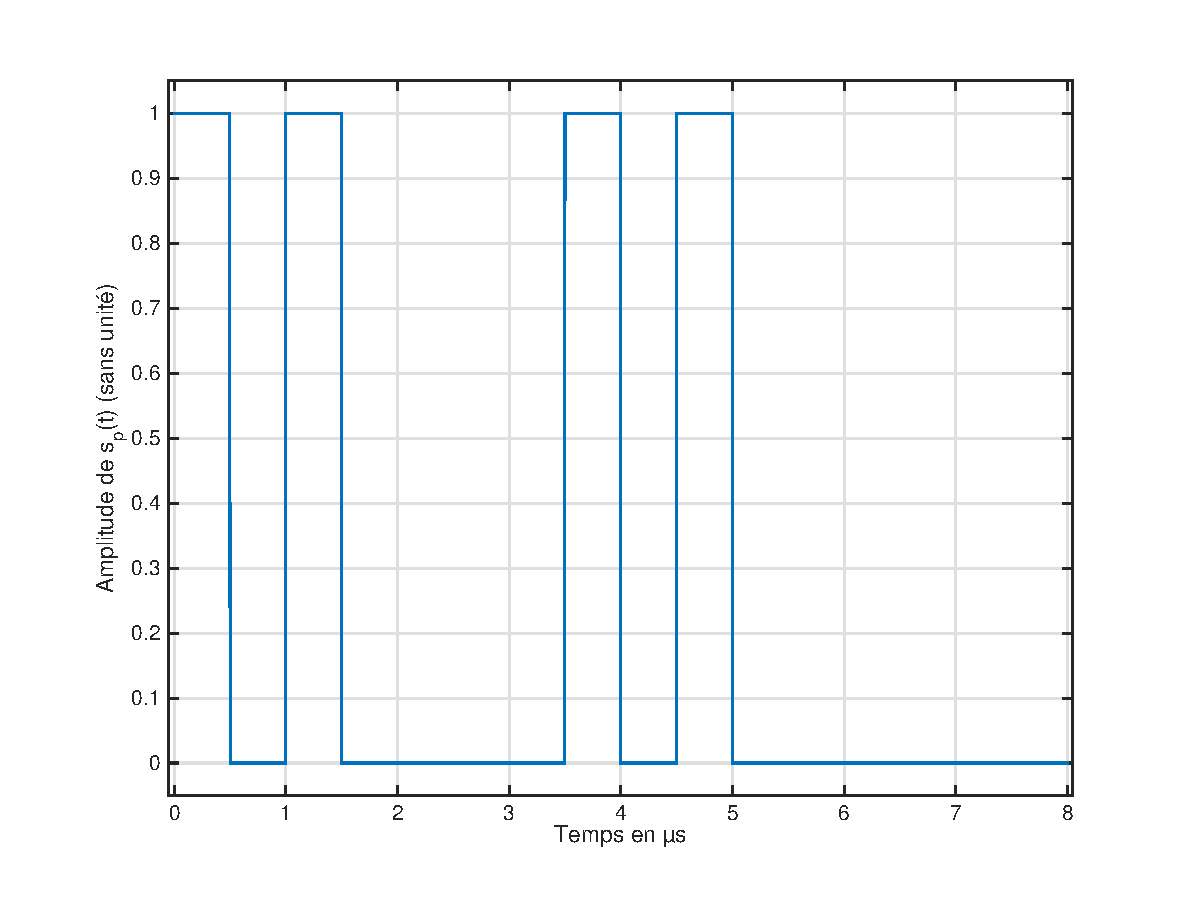
\includegraphics[scale=0.3]{preamble.eps}
        \caption{Préambule débutant les trames ADS-B}
    \end{figure}
    \noindent
    Nous estimons alors par corrélation, les couples $\left(\hat{\delta}_t, \hat{\delta}_f\right)$ tels que $0.75 < \left|\left(\hat{\delta}_t, \hat{\delta}_f\right) \right| \le 1$ avec :
    \[
        \forall \left(\delta_t, \delta_f\right), \rho\left(\delta_t, \delta_f\right) = \frac{\displaystyle\int^{\delta_t + T_p}_{\delta_t}{y_l(t) {s_p}^*\left(t - \delta_t\right) \exp\left(j2\pi\delta_f t\right)dt}}{\displaystyle\sqrt{\int_{0}^{T_p}{\left|s_p(t)\right|^2 dt}}\displaystyle\sqrt{\int^{\delta_t + T_p}_{\delta_t}{\left|y_l(t)\right|^2 dt}}}
    \]
    
    \begin{figure}[h!]
        \centering
        % This file was created by matlab2tikz.
% Minimal pgfplots version: 1.3
%
%The latest updates can be retrieved from
%  http://www.mathworks.com/matlabcentral/fileexchange/22022-matlab2tikz
%where you can also make suggestions and rate matlab2tikz.
%
\definecolor{mycolor1}{rgb}{0.00000,0.44700,0.74100}%
%
\begin{tikzpicture}

\begin{axis}[%
scaled x ticks=false,
xticklabel style={
        /pgf/number format/fixed,
        /pgf/number format/precision=2
},
width=4in,
height=2in,
at={(1.011111in,0.641667in)},
xmin=0.046088,
xmax=0.046106,
xlabel={\footnotesize temps (en $s$)},
ymin=0,
ymax=250
]
\addplot [color=mycolor1,solid,forget plot]
  table[row sep=crcr]{%
0.0460895	45.5411901469428\\
0.04608975	203.769477596621\\
0.04609	166.352036356637\\
0.04609025	25.4950975679639\\
0.0460905	41.5932686861708\\
0.04609075	214.394496198013\\
0.046091	158.094908203901\\
0.04609125	23\\
0.0460915	5.8309518948453\\
0.04609175	26.6270539113887\\
0.046092	10.0498756211209\\
0.04609225	18.3847763108502\\
0.0460925	17.4928556845359\\
0.04609275	21.095023109729\\
0.046093	26.9258240356725\\
0.04609325	202.022275999455\\
0.0460935	161.012421881046\\
0.04609375	41.1096095821889\\
0.046094	28.3196045170126\\
0.04609425	190.157829184075\\
0.0460945	131.026714833274\\
0.04609475	6.08276253029822\\
0.046095	32.649655434629\\
0.04609525	18.3847763108502\\
0.0460955	5\\
0.04609575	21.8403296678416\\
0.046096	22.1359436211787\\
0.04609625	30.5286750449475\\
0.0460965	41.1096095821889\\
0.04609675	32.310988842807\\
0.046097	32.6955654485436\\
0.04609725	17.8885438199983\\
0.0460975	2.82842712474619\\
0.04609775	6.70820393249937\\
0.046098	16.0312195418814\\
0.04609825	185.698680663057\\
0.0460985	177.800449943188\\
0.04609875	188.600106044509\\
0.046099	140.730238399571\\
0.04609925	15\\
0.0460995	16.6433169770932\\
0.04609975	12.6491106406735\\
0.0461	56.3205113613149\\
0.04610025	201.992574120931\\
0.0461005	202.800394476934\\
0.04610075	214.350180779023\\
0.046101	200.68383093812\\
0.04610125	45.8911756223351\\
0.0461015	51.2249938994628\\
0.04610175	207.90863377936\\
0.046102	156.84705926475\\
0.04610225	23.3452350598575\\
0.0461025	49.254441424099\\
0.04610275	217.267116701999\\
0.046103	160.514796825713\\
0.04610325	12.2065556157337\\
0.0461035	16.1245154965971\\
0.04610375	20.8086520466848\\
0.046104	50.7740090991444\\
0.04610425	212.934262156188\\
};
\draw[solid, draw=red] (axis cs:0.0460895,0) rectangle (axis cs:0.0460975,220);
\end{axis}
\end{tikzpicture}%
        \caption{Exemple de détection d'un préambule d'une trame ADS-B dans un signal reçu}
    \end{figure}
    \noindent
    Une fois les synchronisations faites, on reprend la chaîne de communications numériques pour estimer les bits reçus.

\newpage
    \begin{figure}[h!]
        \centering
        \definecolor{mycolor1}{rgb}{0.00000,0.44700,0.74100}%
%
\begin{tikzpicture}[scale=0.60]

\begin{axis}[%
width=5in,
height=4in,
at={(1.011111in,0.641667in)},
xmin=0,
xmax=10,
xlabel={$\left(\frac{E_b}{N_0}\right)_\text{dB}$},
xmajorgrids,
ymode=log,
ymin=1e-06,
ymax=1,
yminorticks=true,
ylabel={TEB},
ymajorgrids,
yminorgrids,
legend style={legend cell align=left,align=left,draw=white!15!black}
]
\addplot [color=mycolor1,solid]
  table[row sep=crcr]{%
0	0.30887875\\
1	0.244597857142857\\
2	0.175844642857143\\
3	0.111914464285714\\
4	0.0593260714285714\\
5	0.0258430357142857\\
6	0.00910785714285714\\
7	0.002759285714286\\
8	0.000774107142857143\\
9	0.00013\\
10	2.0195640679161e-05\\
};
\addlegendentry{TEB pratique};

\addplot [color=red,solid]
  table[row sep=crcr]{%
0	0.0786496035251426\\
1	0.0562819519765415\\
2	0.037506128358926\\
3	0.0228784075610853\\
4	0.0125008180407376\\
5	0.00595386714777866\\
6	0.00238829078093281\\
7	0.000772674815378444\\
8	0.000190907774075993\\
9	3.36272284196175e-05\\
10	3.87210821552204e-06\\
};
\addlegendentry{TEB théorique};

\end{axis}
\end{tikzpicture}%
        \caption{Évolution du TEB en fonction du SNR}
    \end{figure}

    L'estimation temporelle et fréquentielle peuvent être faussées par le bruit introduit ce qui amène à une TEB pratique toujours au-dessus de celle théorique mais qui garde toutefois la même allure.

\part{Traitement / décodage de signaux réels}
    \setcounter{section}{2}
    \setcounter{subsection}{0}
    
    \subsection{Structure des trames ADS-B}
    Les trames ADS-B sont constituées de 120 bits mais les données ADS-B qui contiennent les informations des avions sont mises sur 56 bits (du 40\up{e} au 95\up{e} bit).
    
    \begin{figure}[h!]
    \centering
        \psscalebox{0.57 0.57} % Change this value to rescale the drawing.
            {
            \begin{pspicture}(0,-2.3420312)(26.18,2.3420312)
            \psframe[linecolor=black, linewidth=0.04, dimen=outer](21.6,-1.0660938)(3.6,-1.8660938)
            \psline[linecolor=black, linewidth=0.04](5.4,-1.0660938)(5.4,-1.8660938)
            \psline[linecolor=black, linewidth=0.04](4.6,-1.0660938)(4.6,-1.8660938)
            \psline[linecolor=black, linewidth=0.04](5.2,-1.0660938)(5.2,-1.8660938)
            \psline[linecolor=black, linewidth=0.04](8.0,-1.0660938)(8.0,-1.8660938)
            \psline[linecolor=black, linewidth=0.04](19.0,-1.0660938)(19.0,-1.8660938)
            \rput[bl](3.4,-2.2660937){0}
            \rput[bl](4.4,-2.2660937){8}
            \rput[bl](4.8,-2.2660937){13}
            \rput[bl](5.4,-2.2660937){16}
            \rput[bl](7.8,-2.2660937){40}
            \rput[bl](18.8,-2.2660937){96}
            \rput[bl](21.2,-2.2660937){120}
            \psline[linecolor=black, linewidth=0.04, arrowsize=0.05291666666666667cm 2.0,arrowlength=1.4,arrowinset=0.0]{->}(3.0,-1.8660938)(23.2,-1.8660938)
            \rput[bl](23.4,-2.2660937){temps en $\mu$ s}
            \psline[linecolor=black, linewidth=0.04](12.4,-1.0660938)(12.4,0.33390626)(13.4,0.33390626)
            \psline[linecolor=black, linewidth=0.04](4.0,-1.0660938)(4.0,-0.66609377)(3.2,-0.66609377)
            \psline[linecolor=black, linewidth=0.04](4.8,-1.0660938)(4.8,0.73390627)(3.2,0.73390627)
            \psline[linecolor=black, linewidth=0.04](6.8,-1.0660938)(6.8,2.1339064)(7.8,2.1339064)
            \rput[bl](1.2,-0.86609375){Préambule}
            \rput[bl](0.0,0.73390627){Format de la voie}
            \rput[bl](0.0,0.33390626){descendante}
            \rput[bl](8.0,2.1339064){Adresse OACI de l'avion}
            \rput[bl](13.6,0.13390625){Données ADS-B}
            \psline[linecolor=black, linewidth=0.04](20.2,-1.0660938)(20.2,-0.26609376)(20.6,-0.26609376)
            \rput[bl](20.8,-0.46609375){CRC}
            \end{pspicture}
            }
            \caption{Structure d'une trame ADS-B}
    \end{figure}
    
    Cependant, les messages contenus dans les trames ADS-B peuvent ne pas contenir la même information. Ainsi, un message de position en vol n'aura pas la même structure qu'un message d'identification par exemple.
    
    \vspace{5pt}
    Pour identifier le type du message, nous devons nous intéresser à la valeur du FTC (Format Type Code) codé sur les 5 premiers bits du message. On retrouve alors les messages :
    \begin{itemize}
        \item de position en vol pour un FTC $\in \llbracket 9, 18 \rrbracket \cup \llbracket 20, 22 \rrbracket$
        \item de position au sol pour un FTC $\in \llbracket 5,8 \rrbracket$
        \item d'identification pour un FTC $\in \llbracket 1,4 \rrbracket$
        \item de vitesse en vol pour un FTC $= 19$
    \end{itemize}
    
    \vspace{5pt}
    Les messages de position en vol et d'identification nous donnent respectivement les informations d'altitude, de latitude et de longitude de l'avion ainsi que le nom du vol de l'appareil.
    Pour décoder les messages de position au sol et de vitesse en vol, nous nous sommes aidés d'un document de la FAA sur l'ADS-B [1].
    
    \subsection{Implémentation sur Matlab et optimisations}
    \noindent
    
    Le décodage des trames se fait grâce à la fonction {update\_registres.m} qui appelle en fait deux fonctions. La première, \textsf{bit2registre.m}, met à jour le registre contenant les informations de l'avion (adresse OACI, FTC, nom du vol, vitesses air et par rapport au sol ainsi que le taux de montée ou descente, cap, position et altitude), en contrôlant d'abord le format des trames. Ce registre ne se mettra à jour qu'avec un code CRC correct. La deuxième, \textsf{update\_plots.m}, permet de mettre à jour l'affichage de la trajectoire pour chaque avion afin de marquer seulement la dernière position.
    
    \vspace{10pt}
    
    Les premiers champs du registre sont destinés à stocker l'adresse de l'avion ainsi que son immatriculation. L'adresse OACI se déduit des 24 bits de la trame à partir du bit 16. Une fonction annexe est utilisée pour convertir cette adresse en hexadécimal, plus courante. À partir de cette adresse, il nous est maintenant possible de retrouver l'immatriculation de l'appareil en allant lire dans une base de donnée, \textsf{PlaneInfo.db}, ainsi que sa catégorie. Si l'avion n'est pas dedans, on l'ajoute avec les informations téléchargées depuis \href{http://flightradar24.com}{le site \textit{Flightradar24}} grâce à la fonction \textsf{flightradar\_reader.m}.
    
    \begin{figure}[h!]
    	    \centering
    	    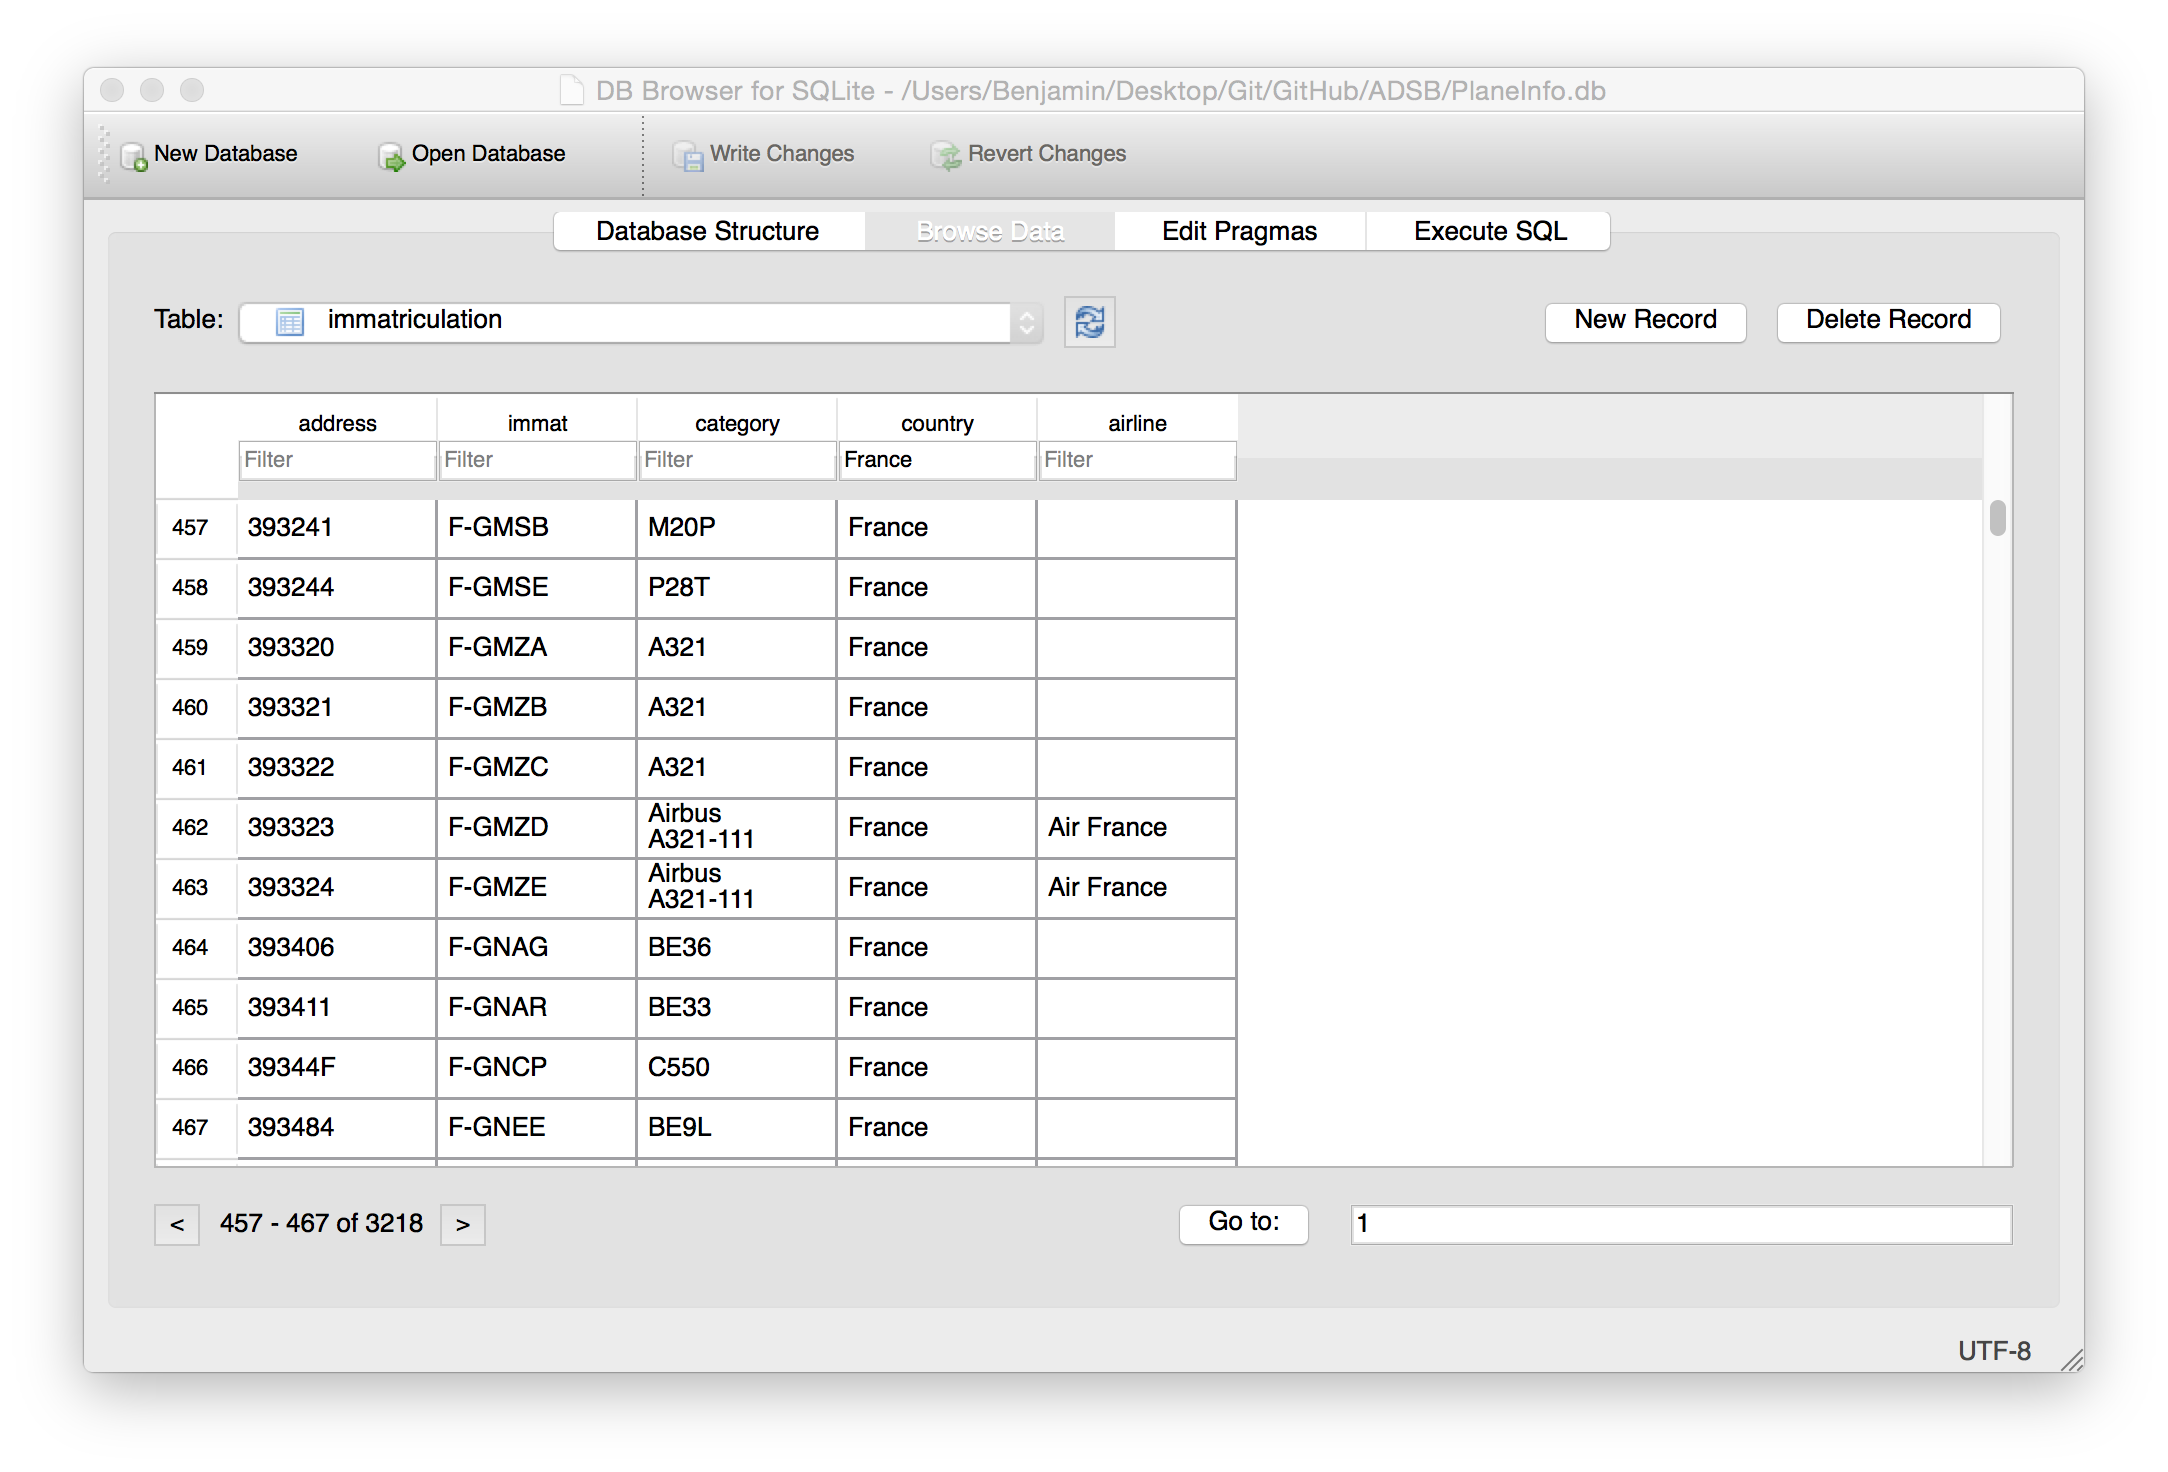
\includegraphics[scale=0.2]{extrait_db.png}
            \caption{Extrait de notre base de données}
    \end{figure}
    
    L'avion identifié à partir des trames contenues dans le fichier \textsf{trames\_20141120.mat} est un Airbus A321 d'Air France immatriculé F-GMZE (adresse hexadécimale = 393324), au décollage à Mérignac, effectuant le vol $\text{n}^{\circ}$ AF255YO.
    Nous avons affiché cette trajectoire avec Google Maps, et OpenStreet Map pour la rapidité d'éxecution par rapport à Google Maps.
    
    \begin{figure}[h!]
        \begin{minipage}[b]{0.45\linewidth}
    	    \centering
    	    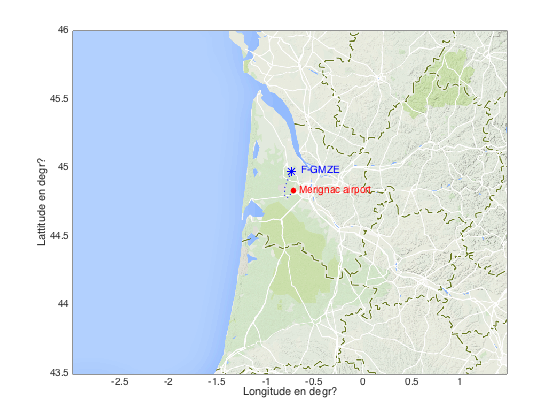
\includegraphics[scale=0.35]{plot_pos_F-GMZE.png}
            \caption{Trajectoire avec Google Maps}
        \end{minipage} \hfill
        \begin{minipage}[b]{.45\linewidth}
    	    \centering
    	    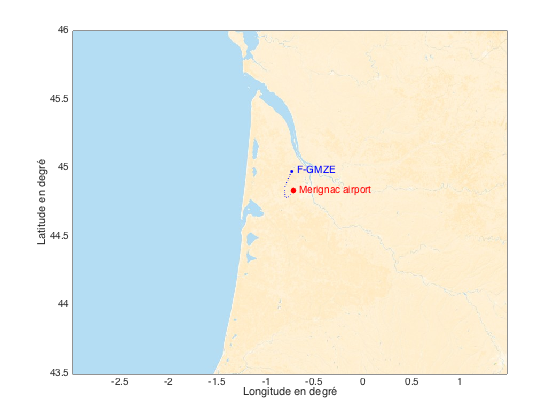
\includegraphics[scale=0.35]{plot_pos_F-GMZE_osm.png}
            \caption{Trajectoire avec OpenStreet Map}
        \end{minipage}
    \end{figure}
    
    \newpage
    Une fois l'affichage des trajectoires réalisé et réussi, nous avons cherché à optimiser notre code. En effet, M\textsc{atlab} est connu pour sa lenteur dès lors que l'on utilise une boucle. C'est pourquoi nous avons essayé d'enlever le plus de boucles possible et appliqué le plus d'opérations sur des matrices.
    
    \vspace{10pt}
    Ainsi, pour l'estimation temporelle, les valeurs du numérateur de la corrélation s'obtient par une convolution entre $s_p$ et la valeur absolue du buffer complexe.
    
    \vspace{10pt}
    De même, pour l'obtention des valeurs des registres, nous avons vectorialisé les conditions [2] ce qui évite un parcours en boucle avec des conditions logiques.

    \vspace{10pt}
\part{Affichage des trajectoires}
    \setcounter{section}{3}
    \setcounter{subsection}{0}
    Le décodage en temps réel se fait avec certaines d'erreurs. La synchronisation fréquentielle reste à implémenter. Celle-ci nous permettrait d'améliorer la détection des avions. En effet, en prenant la valeur absolue de la variable complexe, on cumule simultanément le bruit de la partie réelle et celui de la partie imaginaire.
    
    \vspace{10pt}
    
    La carte en F\textsc{igure} 19 résulte de la fonction \textsf{FOVET.m} et ne fait qu'afficher les trajectoires associées aux adresses hexadécimales. Néanmoins, le code \textsf{ADSB\_part3.m} est bien plus complet et permet de remplir les registres avec toutes les informations contenues dans les trames. Il remplit 2 tableaux :
    \begin{itemize}
    \item Un tableau de structures nommé \textsf{registres} qui se succèdent indépendamment les unes des autres
    \item Un tableau de structures nommé \textsf{plots} qui contiennent les informations regroupées suivant un avion donné et affiché sur la carte.
    \end{itemize}
    
    \vspace{10pt}
    
    En outre, le code \textsf{ADSB\_part3.m} gère également l'affichage des immatriculations implémenté dans la partie 2 et permet de récupérer l'historique des registres.
    
    \vspace{10pt}
    
        \begin{figure}[h!]
        \begin{minipage}[b]{0.45\linewidth}
    	    \centering
    	    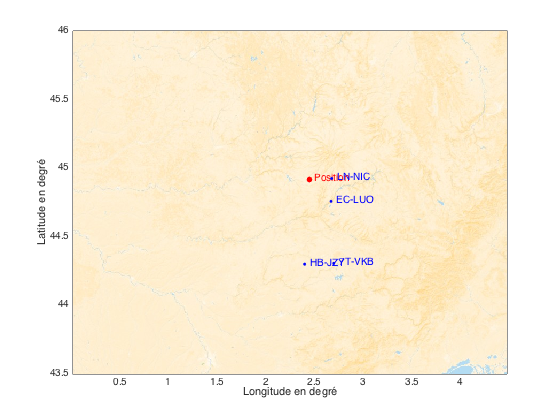
\includegraphics[scale=0.4]{plot_part3.png}
            \caption{Affichage avec \textsf{ADSB\_part3.m}}
        \end{minipage} \hfill
        \begin{minipage}[b]{.45\linewidth}
    	    \centering
    	    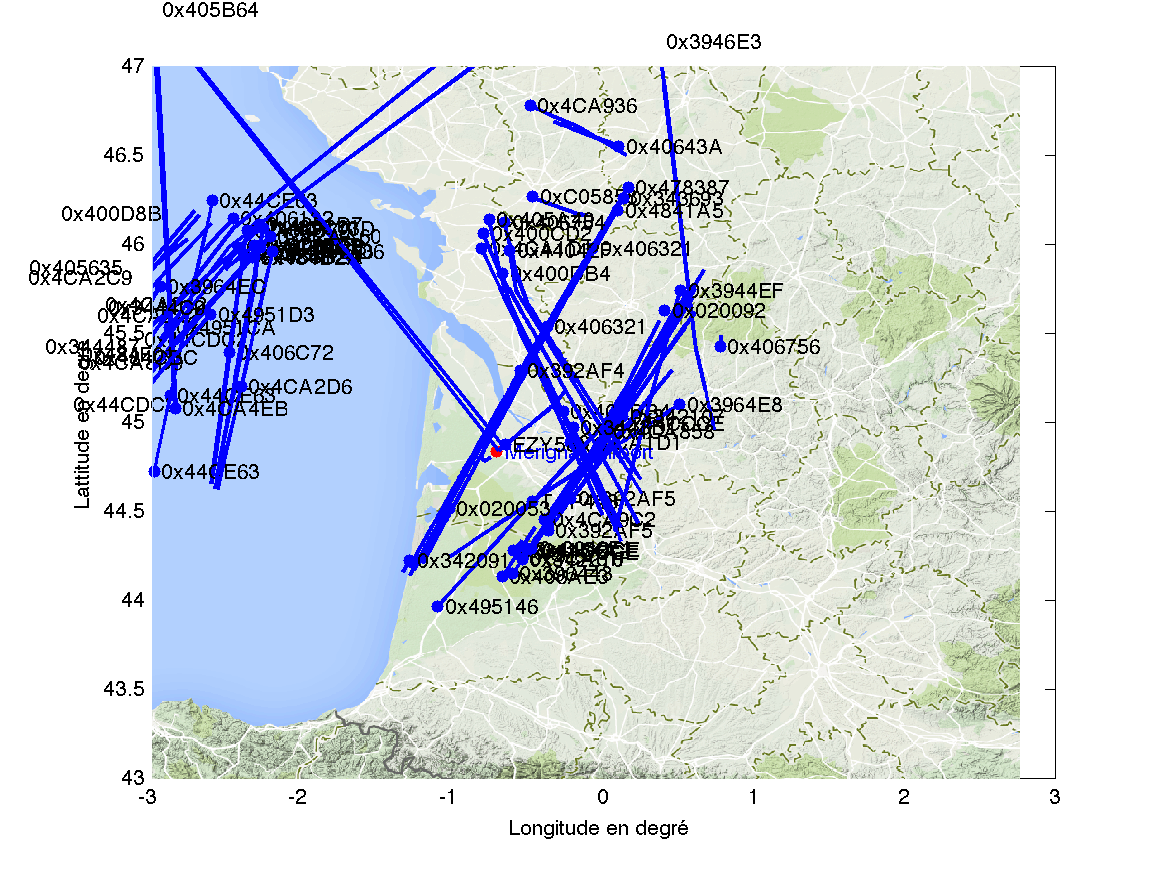
\includegraphics[scale=0.4]{figureEleve.png}
            \caption{Décodage en temps réel effectué}
        \end{minipage}
    \end{figure}
    
    %\begin{figure}[h!]
    %	    \centering
    %	    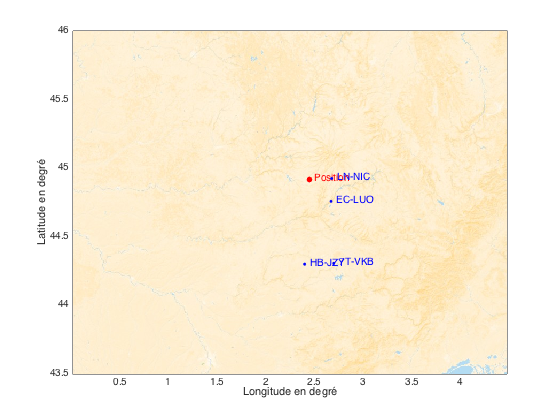
\includegraphics[scale=0.5]{plot_part3.png}
    %        \caption{Affichage avec \textsf{ADSB\_part3.m}}
    %\end{figure}
    \newpage
    \begin{figure}[h!]
    	    \centering
    	    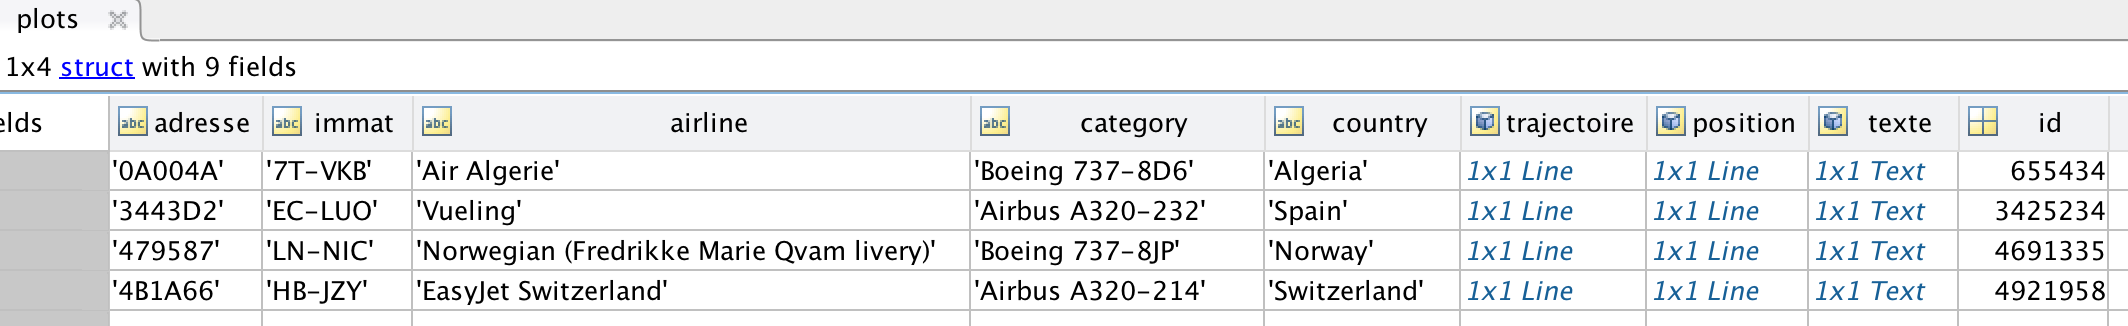
\includegraphics[scale=0.44]{registre_plots.png}
            \caption{Tableau \textsf{plots} récupéré avec \textsf{ADSB\_part3.m}}
    \end{figure}
    
    \begin{figure}[h!]
    	    \centering
    	    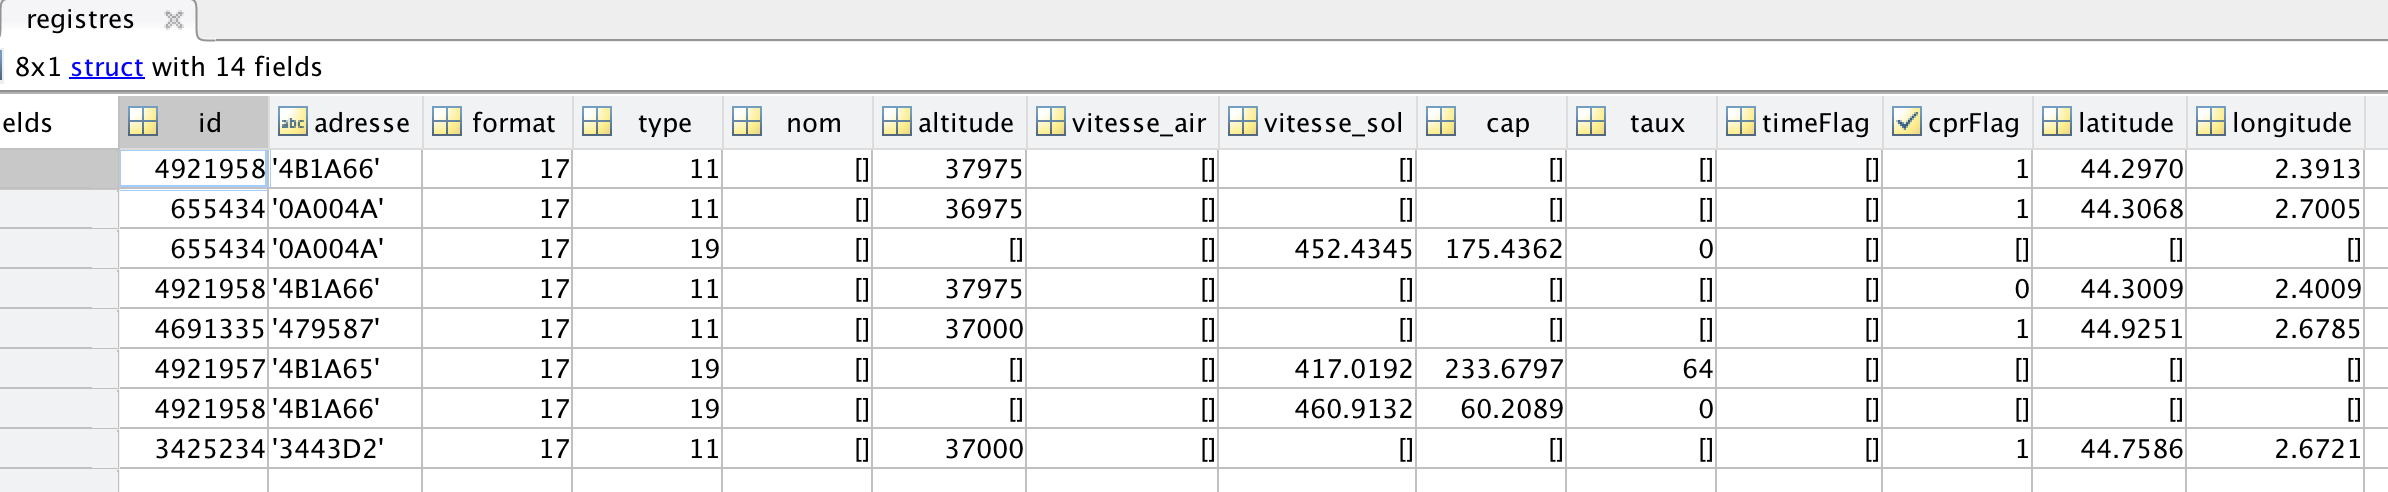
\includegraphics[scale=0.38]{registre_part3.png}
            \caption{Tableau \textsf{registres} récupéré avec \textsf{ADSB\_part3.m}}
    \end{figure}
    
    %\begin{figure}[h!]
    %	    \centering
    %	    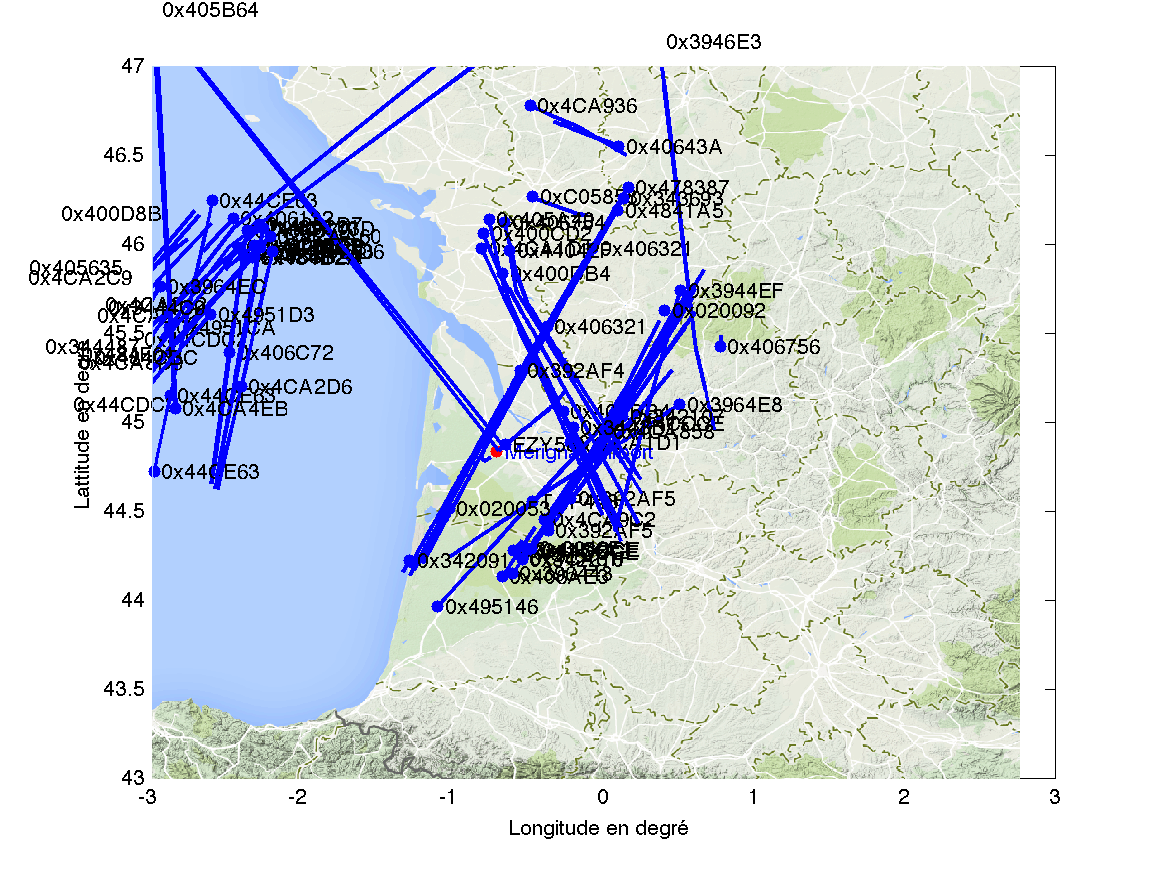
\includegraphics[scale=0.5]{figureEleve.png}
    %        \caption{Premier décodage en temps réel effectué}
    %\end{figure}

    \begin{figure}[h!]
    	    \centering
    	    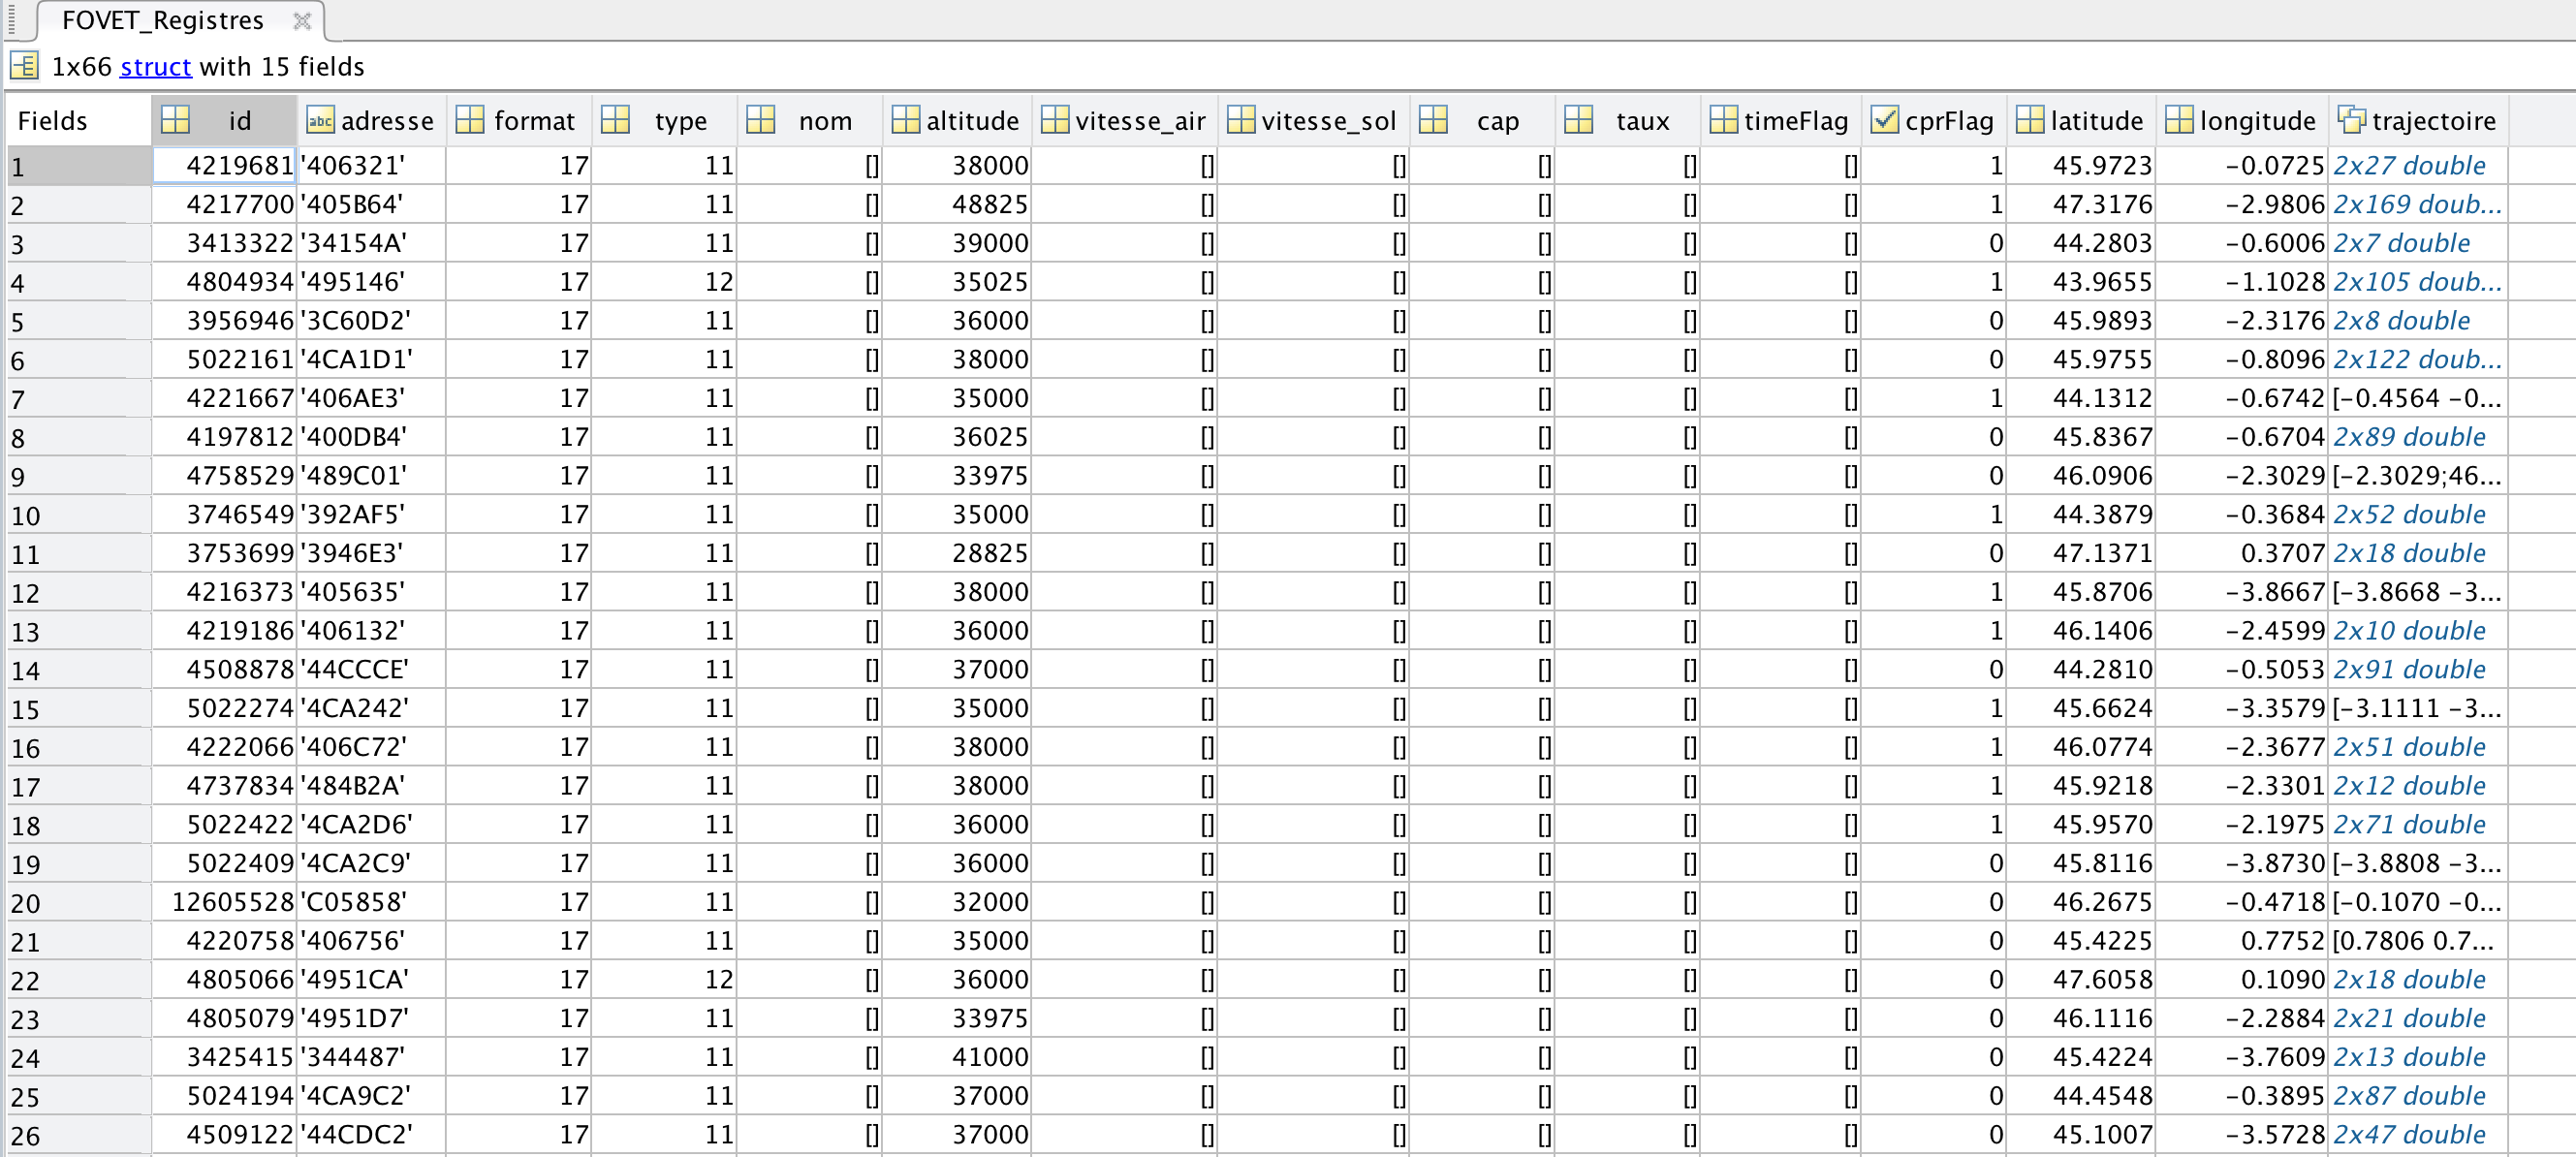
\includegraphics[scale=0.35]{registres.png}
            \caption{Registres récupérés avec \textsf{FOVET.m}}
    \end{figure}
    \noindent
    % Comme on peut le voir dans le registre récupéré ci-dessus, tout n'a pas été implémenté dans la fonction FOVET.m pour le premier décodage, par manque de temps. Toutes les informations étaient néanmoins décodées à ce moment là.

\newpage
\part*{Conclusion}
\addcontentsline{toc}{part}{Conclusion} \markboth{CONCLUSION}{}
Ce projet nous a beaucoup appris tant sur les communications numériques que sur l'implémentation du code sur Matlab, sans oublier l'optimisation du code pour améliorer la rapidité du décodage des trames -- ce qui nous prenait approximativement 10 secondes lors de notre décodage initial ne nous prend désormais environ 0.7 seconde.

\vspace{10pt}
Nous nous sommes également intéressés à d'autres problèmes annexes, comme le décodage de toutes les informations d'identification des avions, grâce à une fonction effectuant des requêtes dans la base de données que nous avons créée, à partir des quatre types de trames possibles qui sont les messages de position en vol et au sol, d'identification et de vitesse.

\vspace{10pt}
Néanmoins, bien que nous ayons gagné une dizaine de secondes en temps d'exécution en modifiant certaines parties du code, nous n'avons implémenté le décodage que de façon sous-optimale, en ne considérant que le décalage temporel.

De plus, il s'exécute avec des erreurs. Pour aller plus loin, nous aurions pu implémenter un détecteur d'erreurs calculant la vitesse de l'avion suivant 2 valeurs consécutives en supposant le temps connu et regarder si cette vitesse est plausible ou non.

% En ajoutant la synchronisation fréquentielle, nous pourrions à coup sûr réduire le nombre d'erreurs au décodage. non ça en rajouterait à coup sûr parce qu'une nouvelle estimation va être faite donc une valeur moins précise :p
% un possible correcteur d'erreur serait de regarder la valeur précédente s'il y en a avec celle actuelle et voir si c'est possible, tout en ayant sauvegarder le tps et ainsi vérifier si la vitesse de l'avion est plausible


\part*{Références}
\addcontentsline{toc}{part}{Références} \markboth{REFERE}{}
\noindent
[1] \href{http://adsb.tc.faa.gov/WG3_Meetings/Meeting30/1090-WP30-21-Appendix_A\%20Mods.pdf}{ \textit{Appendix A, Extended Squitter and TIS-B Formats and Coding Definitions} -- pages 70, 73 à 74}

\noindent
[2] \href{http://www.robogourmet.com/?p=208}{\textit{Speeding Up MATLAB (The RoboGourmet)}}

\subsection*{Services utilisés}
\noindent
\href{http://flightradar24.com}{\textit{Flightradar24}} - pour la vérification des adresses et la requête dans la base de données

\noindent
\href{http://mapbox.com}{\textit{Mapbox}} - pour la génération d'une carte OpenStreet Map
    

\end{document}
